% cSpell:disable

\documentclass[12pt,letterpaper]{report}

% cSpell:disable

\usepackage{style/buthesis}
\usepackage[utf8]{inputenc}

% For page frame
% \usepackage[showframe]{geometry}

\usepackage[usenames,dvipsnames]{xcolor}
\usepackage[
	lambda,
	advantage,
	operators,
	sets,
	landau,
	probability,
	notions,
	logic,
	ff,
	mm,
	primitives,
	events,
	complexity,
	asymptotics,
	keys
]{cryptocode}
\usepackage{appendix}
\usepackage{adjustbox}
\usepackage[ruled]{algorithm}
\usepackage{algorithmicx}
\usepackage[noend]{algpseudocode}
\usepackage{amsmath}
\usepackage{amsfonts}
\usepackage{subcaption}
\usepackage{graphicx}
\usepackage{balance}
\usepackage{diagbox}
\usepackage{mathtools}
\usepackage{nicefrac}
\usepackage{booktabs}
\usepackage{multirow}
\usepackage{bm}
\usepackage{interval}
\usepackage{rotating}
\PassOptionsToPackage{hyphens}{url}
\definecolor{BrightRed}{RGB}{204, 0, 0}
\definecolor{DarkRed}{RGB}{102, 0, 0}
\definecolor{DarkerRed}{RGB}{78, 0, 0}
\definecolor{MidRed}{RGB}{143, 0, 0}

\definecolor{MatplotlibOne}{HTML}{1F77B4}
\definecolor{MatplotlibTwo}{HTML}{FF7F0E}
\definecolor{MatplotlibThree}{HTML}{2CA02C}
\definecolor{MatplotlibFour}{HTML}{D62728}
\definecolor{MatplotlibFive}{HTML}{9467BD}
\definecolor{MatplotlibSix}{HTML}{8C564B}
\definecolor{MatplotlibSeven}{HTML}{E377C2}
\definecolor{MatplotlibEight}{HTML}{7F7F7F}
\definecolor{MatplotlibNine}{HTML}{BCBD22}
\definecolor{MatplotlibTen}{HTML}{17BECF}

\usepackage[
	colorlinks = true,
	linkcolor = DarkRed,
	urlcolor = MidRed,
	citecolor = BrightRed,
]{hyperref}
\usepackage[noabbrev,capitalise]{cleveref} % must be loaded after hyperref

\AtBeginEnvironment{appendices}{\crefalias{chapter}{appendix}}

\usepackage{color}
\usepackage{colortbl}
\usepackage{amsthm}
\usepackage{caption}
\usepackage[all]{nowidow}
\usepackage{hyphenat}
\usepackage[inline]{enumitem}
\usepackage[binary-units]{siunitx}
\usepackage[mathscr]{eucal}
\usepackage{longtable}
\usepackage{makecell}
\usepackage{threeparttable}
\usepackage{textcomp}
\usepackage{array}
\usepackage{calc}
\usepackage[final]{pdfpages}
\usepackage{pax}

\hyphenation{
	Shrink-wrap
	Shma-ti-kov
	SIG-SAC
	SIG-MOD
	Da-ta-ba-ses
	RAN-DOM
	RDB-MS
	Sprin-ger
	Na-ve-ed
	Tho-mas
	VL-DBJ
	Arch-ive
	En-cryp-ted
	Sche-me
	Mi-ro-nov
	Addi-son
	Mi-cha-el
	Kyun-ghy-un
}

\sisetup{
	group-minimum-digits = 4,
	per-mode = symbol
}

\usepackage[
	backend=biber,
	style=alphabetic,
	giveninits=false,
	sorting=ydnt,
	maxbibnames=1000,
	maxalphanames=4
]{biblatex}

\bibliography{bibfile}

\renewcommand*{\mkbibnamegiven}[1]{%
	\ifitemannotation{highlight}
	{\textbf{#1}}
	{#1}
}

\renewcommand*{\mkbibnamefamily}[1]{%
	\ifitemannotation{highlight}
	{\textbf{#1}}
	{#1}
}

\graphicspath{{./graphics/}}

\ifdefined\draft%
	% https://www.overleaf.com/learn/latex/Inserting_Images#Generating_high-res_and_low-res_images
	\usepackage{epstopdf}
	\epstopdfDeclareGraphicsRule{.pdf}{png}{.png}{convert #1 \OutputFile}
	\DeclareGraphicsExtensions{.png,.pdf}
\fi

\usepackage[
	acronym,
	nonumberlist,
	nopostdot,
	nogroupskip
]{glossaries}
\renewcommand*{\glsclearpage}{}
\renewcommand*{\acronymname}{List of Acronyms}

\newglossarystyle{gloTable}
{%
	\newlength\aglslong%
	\settowidth\aglslong{\widthof{\textbf{CCP-ODB}}}

	\newlength\aglsleft%
	\setlength{\aglsleft}{\dimexpr\aglslong+0.1em\relax}

	\newlength\aglsright%
	\setlength{\aglsright}{\widthof{Bidirectional Encoder Representation from Transformer}}

	\newlength\aglscenter%
	\setlength{\aglscenter}{\dimexpr\linewidth-\aglsright-\aglsleft\relax}

	\renewenvironment{theglossary}%
	{
		\begin{center}
			\begin{longtable}{
				>{\raggedright}p{\aglsleft}
				p{\aglscenter}
				>{\raggedright}p{\aglsright}
			}
	}%
	{
			\end{longtable}
		\end{center}
	}%
	% no group headings:
	\renewcommand*{\glsgroupheading}[1]{}%
	% main (level 0) entries displayed in a row
	\renewcommand{\glossentry}[2]{%
		\glsentryitem{##1}\glstarget{##1}{\textbf{\glossentryname{##1}}} & \dotfill & \glossentrydesc{##1} \tabularnewline%
	}%
	% sub-entries (same as main)
	\renewcommand{\subglossentry}[3]{\glossentry{##2}{##3}}%
	% blank row between groups if nogroupskip=false
	\ifglsnogroupskip%
		\renewcommand*{\glsgroupskip}{}%
	\else
		\renewcommand*{\glsgroupskip}{ & & \tabularnewline}%
	\fi
}
\setglossarystyle{gloTable}

\renewcommand*{\glsclearpage}{}
\makeglossaries%
\glsaddall%

\renewcommand*{\glstextformat}[1]{\textcolor{DarkerRed}{#1}}

\newcommand{\crypte}{Crypt\ensuremath{\epsilon}}
\newcommand{\epsolute}{\ensuremath{\mathcal{E}}p\-so\-lu\-te}

\newcommand{\record}{\ensuremath{r}}
\newcommand{\recordID}{\ensuremath{\record^\mathsf{ID}}}
\newcommand{\recordIDPrime}{\ensuremath{{}^\mathsf{ID}\record^\prime}}
\newcommand{\querySet}{\ensuremath{\mathcal{Q}}}
\newcommand{\queryKey}{\ensuremath{K}}

\newcommand{\domainSize}{\ensuremath{N}}
\newcommand{\dataSize}{\ensuremath{n}}
\newcommand{\oramsNumber}{\ensuremath{m}}

\newcommand{\user}{\ensuremath{\mathscr{U}}}
\newcommand{\client}{\ensuremath{\mathscr{C}}}
\newcommand{\server}{\ensuremath{\mathscr{S}}}

\newcommand{\protocol}{\ensuremath{\Pi}}
\newcommand{\protocolSetup}{\ensuremath{\protocol_{\mathsf{setup}}}}
\newcommand{\protocolQuery}{\ensuremath{\protocol_{\mathsf{query}}}}
\newcommand{\protocolNoGamma}{\ensuremath{\protocol_{\mathsf{no-}\gamma}}}
\newcommand{\protocolGamma}{\ensuremath{\protocol_\gamma}}

\newcommand{\searchKey}{\textsf{SK}}
\newcommand{\searchKeyDomain}{\ensuremath{\mathcal{X}}}

\newcommand{\serverDS}{\ensuremath{\mathcal{DS}}}
\newcommand{\indexI}{\ensuremath{\mathcal{I}}}
\newcommand{\database}{\ensuremath{\mathcal{D}}}
\newcommand{\databaseDef}{\ensuremath{\database = \allowbreak \{(\record_1, \allowbreak \recordID_1, \allowbreak \searchKey_1), \allowbreak \ldots, \allowbreak (\record_\dataSize, \allowbreak \recordID_\dataSize, \allowbreak \searchKey_\dataSize)\}}}
\newcommand{\fanout}{\ensuremath{k}}

\newcommand{\oram}{\ensuremath{\textsc{ORAM}}}
\newcommand{\oramProgram}{\ensuremath{\mathbf{y}}}
\newcommand{\oramRead}{\ensuremath{\mathbf{r}}}
\newcommand{\oramWrite}{\ensuremath{\mathbf{w}}}

\newcommand{\efficiencyCoefficient}{\ensuremath{a_1}}
\newcommand{\efficiencyOffset}{\ensuremath{a_2}}

\DeclareDocumentCommand{\algo}{ m g }{%
	{%
		\textsc{#1}%
		\IfNoValueF{#2}{\ensuremath{\left( #2 \right)}}%
	}%
}

\DeclareDocumentCommand{\query}{ g g }{%
	{%
		\IfValueTF{#2}%
			{\ensuremath{q_{\interval{#1}{#2}}}}%
			{
				\IfValueTF{#1}%
					{\ensuremath{q_{#1}}}%
					{\ensuremath{q}}
			}%
	}%
}

\newcommand{\adversary}{\ensuremath{\mathcal{A}}}
\newcommand{\leakage}[1]{\ensuremath{\mathcal{L}_{\textsf{#1}}}}
\renewcommand{\simulator}{\textsc{Sim}}
\DeclareDocumentCommand{\view}{ g g }{%
	{%
		\IfValueTF{#2}%
			{\ensuremath{\algo{View}_{#1} \left( #2 \right)}}%
			{
				\IfValueTF{#1}%
					{\ensuremath{\algo{View}_{#1}}}%
					{\ensuremath{\algo{View}}}
			}%
	}%
}

\providecommand{\bigTheta}[1]{\ensuremath{\Theta \left( #1 \right)}}

\newcommand{\fromNtoM}[3]{\ensuremath{#1_#2, \allowbreak \ldots, \allowbreak #1_#3}}
\newcommand{\probability}[1]{\ensuremath{\textnormal{Pr}\left[ #1 \right]}} % chktex 35
\newcommand{\efficiency}[2]{\ensuremath{\left( \bigO{ #1 }, \ifthenelse{\equal{#2}{0}}{#2}{\bigO{ #2 }} \right)}}
\newcommand{\semitransp}[2][35]{\color{fg!#1}#2}

\newcommand{\BPlus}{B\raisebox{.35\height}{\scalebox{.8}{+}}}

\newtheorem{definition}{Definition}[section]
\newtheorem{remark}{Remark}[section]

\newtheorem{theorem}{Theorem}[section]
\newtheorem{claim}[theorem]{Claim}
\newtheorem{lemma}[theorem]{Lemma}
\newtheorem{proposition}[theorem]{Proposition}
\newtheorem{corollary}[theorem]{Corollary}
\newtheorem{observation}[theorem]{Observation}
\newtheorem{fact}[theorem]{Fact}
\newtheorem{example}[theorem]{Example}

% Add bidirectional arrow to cryptocode
\makeatletter
	\newcommandx*{\sendmessageboth}[2][1=<->]{%
		\sendmessage{#1}{#2}%
	}
	\WithSuffix\newcommand\sendmessageboth*[2][\pcdefaultmessagelength]{%
		\begingroup%
			\renewcommand{\@pcsendmessagetop}{\let\halign\@pc@halign$\begin{aligned}#2\end{aligned}$}% chktex 21
			\sendmessage{<->}{length=#1}%
		\endgroup%
	}
	\renewcommand{\pccomment}[1]{{\rhd\;\text{\scriptsize#1}}} % chktex 21
\makeatother

\newcommand{\pcinput}[1]{\textbf{Input:}\ #1}
\newcommand{\pcouput}[1]{\textbf{Output:}\ #1}

\definecolor{lightGrey}{RGB}{220,220,220}

% https://tex.stackexchange.com/a/1248/97712
% https://tex.stackexchange.com/a/268845/97712
\makeatletter
	\let\orgdescriptionlabel\descriptionlabel%
	\renewcommand*{\descriptionlabel}[1]{%
		\let\orglabel\label%
		\let\label\@gobble% chktex 21
		\phantomsection%
		\protected@edef\@currentlabel{#1\unskip}% chktex 21
		\let\label\orglabel
		\orgdescriptionlabel{#1}%
	}
\makeatother

% https://github.com/arnomi/cryptocode/issues/5
\AtBeginDocument{
	\pcfixhyperref%
	\makeatletter
		\crefformat{@pclinenumber}{line~#2#1#3}
		\Crefformat{@pclinenumber}{Line~#2#1#3}
		\crefrangeformat{@pclinenumber}{lines~#3#1#4 to~#5#2#6}
		\Crefrangeformat{@pclinenumber}{Lines~#3#1#4 to~#5#2#6}
	\makeatother
}

\newcommand{\domain}{\mathcal{D}}
\newcommand{\leak}{\mathcal{L}}
\newcommand{\setup}{\algo{KGen}}
\newcommand{\encrypt}{\algo{Enc}}
\newcommand{\compare}{\algo{Cmp}}
\newcommand{\tapegen}{\algo{TapeGen}}
\newcommand{\Csharp}{%
	{\settoheight{\dimen0}{C}C\kern-.05em \resizebox{!}{\dimen0}{\raisebox{\depth}{\#}}} % chktex 41
}

\newcommand{\FOne}{\ensuremath{\text{F}_1}}

% https://tex.stackexchange.com/a/267089/97712
\newcommand{\printpublication}[1]{\AtNextCite{\defcounter{maxnames}{99}}\fullcite{#1}}


% cSpell:ignore rdbms dcpe faiss trec

\newacronym%
	{vm}
	{VM}
	{Virtual Machine}

\newacronym%
	{ore}
	{ORE}
	{Order-Revealing Encryption}

\newacronym%
	{prf}
	{PRF}
	{Pseudo-Random Function}

\newacronym%
	{prp}
	{PRP}
	{Pseudo-Random Permutation}

\newacronym%
	{sse}
	{SSE}
	{Searchable Symmetric Encryption}

\newacronym%
	{prg}
	{PRG}
	{Pseudo-Random Generator}

\newacronym%
	{pph}
	{PPH}
	{Property-Preserving Hash}

\newacronym%
	{ope}
	{OPE}
	{Order-Preserving Encryption}

\newacronym%
	{dp}
	{DP}
	{Differential Privacy}

\newacronym%
	{oram}
	{ORAM}
	{Oblivious Random Access Machine}

\newacronym%
	{hg}
	{HG}
	{hypergeometric probability distribution}

\newacronym%
	{lpa}
	{LPA}
	{Laplacian Perturbation Algorithm}

\newacronym%
	{sql}
	{SQL}
	{Structured Query Language}

\newacronym%
	{io}
	{I/O}
	{Input / Output}

\newacronym%
	{rdbms}
	{RDBMS}
	{Relational Database Management System}

\newacronym%
	{knn}
	{\knn}
	{$k$-nearest-neighbor}

\newacronym%
	{dcpe}
	{DCPE}
	{Distance Comparison Preserving Encryption}

\newacronym%
	{cdpodb}
	{CDP-ODB}
	{Computationally \acrshort{dp} Outsourced Database System}

\newacronym%
	{trec}
	{TREC}
	{Text Retrieval Conference}

\newacronym%
	{mrr}
	{MRR}
	{Mean Reciprocal Rank}

\newacronym%
	{dcg}
	{DCG}
	{Discounted Cumulative Gain}

\newacronym%
	{faiss}
	{FAISS}
	{Facebook AI Similarity Search}

\newacronym%
	{gpu}
	{GPU}
	{Graphics Processing Unit}

\newacronym%
	{hipaa}
	{HIPAA}
	{Health Insurance Portability and Accountability Act}

\newacronym%
	{tee}
	{TEE}
	{Trusted Execution Environment}

\newacronym%
	{sgx}
	{SGX}
	{Software Guard Extensions}

\newacronym%
	{ap}
	{AP}
	{Access Pattern}

\newacronym%
	{cv}
	{CV}
	{Communication Volume}

\newacronym%
	{fpga}
	{FPGA}
	{Field-Programmable Gate Array}

\newacronym%
	{cdf}
	{CDF}
	{Cumulative Distribution Function}

\newacronym%
	{cpu}
	{CPU}
	{Central Processing Unit}

\newacronym%
	{kvs}
	{KVS}
	{Key-Value Store}

\newacronym%
	{brc}
	{BRC}
	{Best Range cover}

\newacronym%
	{ssd}
	{SSD}
	{Solid State Drive}


\begin{document}

	% cSpell:ignore pdftitle pdfsubject pdfkeywords pdfcreator pdfproducer dvips Epsolute

\title{Secure and Efficient Query Processing in Outsourced Databases}
\author{Dmytro Bogatov}

\degree=2

\prevdegrees{
	B.S., Worcester Polytechinc Institute, 2017 \\
	M.S., Boston University, 2019
}

\department{Graduate School of Arts and Sciences}

\defenseyear{2022}
\degreeyear{2022}

\reader{First}{George Kollios, Ph.D.}{Professor of Computer Science}
\reader{Second}{Leonid Reyzin, Ph.D.}{Professor of Computer Science}
\reader{Third}{Manos Athanassoulis, Ph.D.}{Assistant Professor of Computer Science}
\reader{Fourth}{Adam O'Neil, Ph.D.}{Assistant Professor of Computer Science}

\numadvisors=1
\majorprof{George Kollios, Ph.D.}{Professor of Computer Science}

% TODO conditionally uncomment for print
% \buecethesistitleboxpage

\hypersetup{
	pdfauthor   = {Dmytro Bogatov <dmytro@bu.edu>},
	pdftitle    = {Secure and Efficient Query Processing in Outsourced Databases},
	pdfsubject  = {Doctoral Dissertation Prospectus},
	pdfkeywords = {OPE, ORE, Range Query Protocols, Epsolute, kNN},
	pdfcreator  = {LaTeX with hyperref package},
	pdfproducer = {dvips + ps2pdf}
}


	\ifthenelse{1=1}{
		\maketitle
	}{
		Not particularly proud, but it seems necessary.
		I use pandoc to convert Tex to text and then run some plain text analysis.
		For some reason pandoc fails for the \\maketitle statement.
		However, it is not smart enough to deduce that this condition is always true, while Tex is.
	}
	\cleardoublepage%

	\copyrightpage%
	\cleardoublepage%

	% TODO conditionally uncomment
	\approvalpagewithcomment%
	% \approvalpage%
	\cleardoublepage%

	\IfFileExists%
		{frontmatter/quote.tex}
		{
			\newpage
			Quote

			\cleardoublepage%
		}
		{}

	\IfFileExists%
		{frontmatter/acknowledgments.tex}
		{
			\newpage
			\section*{\centerline{Acknowledgments}}

	First and foremost, I want to thank my advisor, George Kollios, for his guidance and continued support throughout my doctorate journey, from the day he accepted me to his lab to this day.
	I am honored to call him and his family my friends.
	I also thank Leo Reyzin for the time and effort he spent helping me with my work, and for the many cups of coffee and long life talks we have had over these years.
	I want to especially note the many hours-long philosophical discussions with Manos Athanassoulis --- the discussions I truly enjoyed.
	In the heat of the our debates we have lived up to the Ph.\ part of our degrees.
	My special thanks go to Adam O'Neil for his countless contributions to my works.
	He has been an invaluable co-author, contributor, reviewer and friend.

	I would like to express my gratitude to my closest ally in this life, my beloved wife, Daria Bogatova.
	There is not a single piece fo writing I did without your review, not a single figure I crafted without your keen eye refining the tiniest details, from fonts to colors.
	Even the source code of this very thesis has been branched off of your work Bachelor work \cite{dasha-thesis}.
	You are the first to listen to my ideas, and the first to support them unconditionally.

	I would particularly like to thank my bosom friend, roommate and a fellow Doctor, Oleksandr Narykov.
	Living in Boston will not be the same without you, and I hope your career will bring you here in no time.

	My deepest appreciation goes to my colleagues and co-authors, Georgios Kellaris, Björn Tackmann, Kaoutar Elkhiyaoui, Angelo De Caro, Kobbi Nissim and Hamed Zamani.
	It has been a great pleasure and a rewarding experience working with you.
	Your input in my work has been indispensable.

	I am deeply grateful to my fellow Amazonians, Kiran Chinta, Sriram Krishnamurthy, Naresh Chainani, Ramchandra Kulkarni and Abhishek Rai Sharma with whom I shared a number of internships.
	I am very excited to join the team full-time!

	% - George
	% - Leo
	% - Manos
	% - Adam
	% - Dasha + citation
	% - Sasha
	% - Kellaris
	% - Bjorn and IBMers
	% - Kobbi, Hamed
	% - Kiran, Sriram, Naresh
	% - Family
	% - Larger family
	% - Cat

			\cleardoublepage%
		}
		{}

	\begin{abstractpage}
		As organizations struggle with processing vast amounts of information, outsourcing sensitive data to third parties becomes necessary.
Various cryptographic techniques are used in outsourced database systems to ensure data privacy while allowing for efficient querying.
In this prospectus, I propose a definition and components of a new secure and efficient outsourced database system, which answers various types of queries, with different privacy guarantees in different security models.

I start with my survey work on five order-preserving and order-revealing encryption schemes that can be used directly in many database indices, such as the B+ tree, and five range query protocols with various tradeoffs in terms of security and efficiency.
This work systematizes the state-of-the-art range query solutions in a snapshot adversary setting and offers some non-obvious observations regarding the efficiency of the constructions.

I then follow with a recently published work, \epsolute{} --- an efficient range query engine in a persistent adversary model.
In this work, we achieve security in a setting with a much stronger adversary where she can continuously observe everything on the server, and leaking even the result size can enable a reconstruction attack.
We propose a definition, construction, analysis, and experimental evaluation of a system that provably hides both access pattern and communication volume while remaining efficient.

Finally, I analyze the secure \acrlong{knn} queries, in which the security is achieved similarly to \acrshort{ope}/\acrshort{ore} solutions --- encrypting the input with an approximate \acrlong{dcpe} scheme so that the inputs are perturbed, but the query algorithm still produces accurate results.
In this work, we adapt a property-preserving encryption scheme and run a series of experiments to observe the tradeoff between search accuracy and attack effectiveness.
We use \acrshort{trec} datasets and queries for the search and track the accuracy metrics such as \acrshort{mrr} and \acrshort{dcg}.
For the attacks, we build an \acrshort{lstm} model that trains on the correlation between a sentence and its embedding and then predicts words from the embedding.

	\end{abstractpage}
	\cleardoublepage%

	\IfFileExists%
		{frontmatter/preface.tex}
		{
			\newpage
			\section*{Preface}

Preface

			\cleardoublepage%
		}
		{}

	\setcounter{tocdepth}{4}
	\phantomsection%
	\addcontentsline{toc}{chapter}{Contents}
	\tableofcontents
	\cleardoublepage%

	\newpage
	\listofalgorithms%
	\addcontentsline{toc}{chapter}{\listalgorithmname}
	\cleardoublepage%

	\newpage
	\listoftables
	\addcontentsline{toc}{chapter}{\listtablename}
	\cleardoublepage%

	\newpage
	\listoffigures
	\addcontentsline{toc}{chapter}{\listfigurename}
	% \cleardoublepage%

	\addtocontents{toc}{\protect\contentsline{chapter}{\protect{}List of Acronyms}{xvi}{link}}
	\printglossaries%
	\cleardoublepage%

	\newpage
	\endofprelim%
	\cleardoublepage%

	\section{Introduction}

	Secure outsourced database systems aim at helping organizations outsource their data to untrusted third parties, without compromising data confidentiality or query efficiency.
	The main idea is to encrypt the data records before uploading them to an untrusted server along with an index data structure that governs which encrypted records to retrieve for each query.
	While strong cryptographic tools can be used for this task, existing implementations such as CryptDB \cite{crypt-db}, Cipherbase \cite{cipherbase-daas}, StealthDB \cite{stealth-db} and TrustedDB \cite{trusted-db} try to optimize performance but do not provide strong security guarantees when answering queries.
	Indeed, a series of works \cite{multidimensional-range-queries, inference-attack-islam-14, leakage-abuse-attacks-cash-15, inference-attacks-naveed-15, generic-attacks-kellaris, attacks-tao-of-inference, grubbs-attacks, access-pattern-disclosure, attacks-improved-reconstruction} demonstrate that these systems are vulnerable to a variety of reconstruction attacks.
	That is, an adversary can fully reconstruct the distribution of the records over the domain of the indexed attribute.
	This weakness is prominently due to the \emph{access pattern leakage}: the adversary can tell if the same encrypted record is returned on different queries.

	More recently, \cite{generic-attacks-kellaris, state-of-uniform, attacks-improved-reconstruction, pump-volume-attacks, volume-range-attacks} showed that reconstruction attacks are possible even if the systems employ heavyweight cryptographic techniques that hide the access patterns, such as homomorphic encryption \cite{arbitrary-functions-encrypted, fully-homomorphic-encryption} or \acrfull{oram} \cite{oram-theory, oram-original}, because they leak the size of the result set of a query to the server (this is referred to as \emph{communication volume leakage}). % chktex 2
	Thus, even some recent systems that provide stronger security guarantees like ObliDB \cite{oblidb}, Opaque \cite{opaque} and Oblix \cite{oblix} are susceptible to these attacks. % chktex 2
	This also means that no outsourced database system can be both optimally efficient and privacy-preserving: secure outsourced database systems should not return the exact number of records required to answer a query.

	We take the next step towards designing secure outsourced database systems by presenting novel constructions that strike a provable balance between efficiency and privacy.
	First, to combat the access pattern leakage, we integrate a layer of \acrshort{oram} storage in our construction.
	Then, we bound the communication volume leakage by utilizing the notion of \acrfull{dp} \cite{differential-privacy-original}.
	Specifically, instead of returning the exact number of records per query, we only reveal perturbed query answer sizes by adding random encrypted records to the result so that the communication volume leakage is bounded.
	Our construction guarantees privacy of any single record in the database which is necessary in datasets with stringent privacy requirements.
	In a medical \acrshort{hipaa}-compliant setting, for example, disclosing that a patient exists in a database with a rare diagnosis correlating with age may be enough to reveal a particular individual.

	The resulting mechanism achieves the required level of privacy, but implemented na\"{\i}vely the construction is prohibitively slow.
	We make the solution practical by limiting the amount of noise and the number of network roundtrips while preserving the privacy guarantees.
	We go further and present a way to parallelize the construction, which requires adapting noise-generation algorithms to maintain differential privacy requirements.

	Using our system, we have run an extensive set of experiments over cloud machines, utilizing large datasets --- that range up to 10 million records --- and queries of different sizes, and we report our experimental results on efficiency and scalability.
	We compare against best possible solutions in terms of efficiency (conventional non-secure outsourced database systems on unencrypted data) and against an approach that provides optimal security (retrieves the full table from the cloud or runs the entire query obliviously with maximal padding).
	We report that our solution is very competitive against both baselines.
	Our performance is comparable to that of unsecured plain-text optimized database systems (like MySQL and PostgreSQL): while providing strong security and privacy guarantees, we are only 4 to 8 times slower in a typical setting.
	Compared with the optimally secure solution, a linear scan (downloading all the records), we are 18 times faster in a typical setting and even faster as database sizes scale up.

	\smallskip

	To summarize, our contributions in this work are as follows:
	\begin{itemize}
		\item
			We present a new model for a \emph{differentially private} outsourced database system, \acrshort{cdpodb}, its security definition, query types, and efficiency measures.
			In our model, the adversarial honest-but-curious server cannot see the record values, access patterns, or exact communication volume.

		\item
			We describe a novel construction, \epsolute{}, that satisfies the proposed security definition, and provide detailed algorithms for both range and point query types.
			In particular, to conceal the access pattern and communication volume leakages, we provide a secure storage construction, utilizing a combination of \acrlong{oram} \cite{oram-theory, oram-original} and differentially private sanitization \cite{non-interactive-database-privacy}.
			Towards this, we maintain an index structure to know how many and which objects we need to retrieve.
			This index can be stored locally for better efficiency (in all our experiments this is the case), but crucially, it can also be outsourced to the adversarial server and retrieved on-the-fly for each query.

		\item
			We improve our generic construction to enable parallelization within a query.
			The core idea is to split the storage among multiple \acrshortpl{oram}, but this requires tailoring the overhead required for differential privacy proportionally to the number of \acrshortpl{oram}, in order to ensure privacy.
			We present practical improvements and optimization techniques that dramatically reduce the amount of fetched noise and the number of network roundtrips.

		\item
			Finally, we provide and open-source a high-quality C++ implementation of our system.
			We have run an extensive set of experiments on both synthetic and real datasets to empirically assess the efficiency of our construction and the impact of our improvements.
			We compare our solutions to the na\"{\i}ve approach (linear scan downloading all data every query), oblivious processing and maximal padding solution (Shrinkwrap \cite{shrinkwrap}), and to a non-secure regular \acrshort{rdbms} (PostgreSQL and MySQL), and we show that our system is very competitive.
	\end{itemize}

	\subsection{Related Work}

		We group the related secure databases, engines, and indices into three categories
		\begin{enumerate*}[label={(\roman*)}]
			\item systems that are oblivious or volume-hiding and do not require \acrfull{tee},
			\item constructions that rely on \acrshort{tee} (usually, Intel \acrshort{sgx}),
			\item solutions that use property-preserving or semantically secure encryption and target primarily a snapshot adversary.
		\end{enumerate*}
		\emph{We claim that \epsolute{} is the most secure and practical range- and point-query engine in the outsourced database model, that protects both \acrfull{ap} and \acrfull{cv} using \acrlong{dp}, while not relying on \acrshort{tee}, linear scan or padding result size to the maximum.}

		\paragraph*{Obliviousness and volume-hiding without enclave}

			This category is the most relevant to \epsolute{}, wherein the systems provide either or both \acrshort{ap} and \acrshort{cv} protection without relying on \acrshort{tee}.
			\crypte{} \cite{crypte} is a recent end-to-end system executing ``\acrshort{dp} programs''.
			\crypte{} has a different model than \epsolute{} in that it assumes two non-colluding servers, an adversarial querying user (the analyst), and it uses \acrshort{dp} to protect the privacy of an individual in the database, which includes volume-hiding for aggregate queries.
			\crypte{} also does not consider oblivious execution and attacks against the \acrshort{ap}.
			Shrinkwrap \cite{shrinkwrap} (and its predecessor SMCQL \cite{smcql}) is an excellent system designed for complex queries over federated and distributed data sources.
			In Shrinkwrap, \acrshort{ap} protection is achieved by using oblivious operators (linear scan and sort) and \acrshort{cv} is concealed by adding fake records to intermediate results with \acrshort{dp}.
			Padding the result to the maximum size first and doing a linear scan over it afterwards to ``shrink'' it using \acrshort{dp}, is much more expensive than in \epsolute{}, however.
			In addition, in processing a query, the worker nodes are performing an $O(n \log{n})$ cost oblivious sorting, where $n$ is the maximum result size (whole table for range query), since they are designed to answer more general complex queries.
			SEAL \cite{seal} offers adjustable \acrshort{ap} and \acrshort{cv} leakages, up to specific bits of leakage.
			SEAL builds on top of Logarithmic-SRC \cite{practical-range-search}, splits storage into multiple \acrshortpl{oram} to adjust \acrshort{ap}, and pads results size to a power of 2 to adjust \acrshort{cv}.
			\epsolute{}, on the other hand, fully hides the \acrshort{ap} and uses \acrshort{dp} with its guarantees to pad the result size.
			PINED-RQ \cite{pined-rq} samples Laplacian noise right in the B+ tree index tree, adding fake and removing real pointers according to the sample.
			Unlike \epsolute{}, PINED-RQ allows false negatives (i.e., result records not included in the answer), and does not protect against \acrshort{ap} leakage.
			On the theoretical side, \textcite{differential-obliviousness} (followed by \textcite{differential-obliviousness-followup}) treat the \acrshort{ap} itself as something to protect with \acrshort{dp}.
			\cite{differential-obliviousness} introduces a notion of differential obliviousness that is admittedly weaker than the full obliviousness used in \epsolute{}. % chktex 2
			Most importantly, \cite{differential-obliviousness} ensures differential privacy w.r.t.~the \acrshort{oram} only, while \epsolute{} ensures \acrshort{dp} w.r.t.~the entire view of the adversary. % chktex 2

		\paragraph*{Enclave-based solutions}

			Works in this category use trusted execution environment (usually, \acrshort{sgx} enclave).
			These works are primarily concerned with the \acrshort{ap} protection for both trusted and untrusted memory, unlike \epsolute{} which also protects \acrshort{cv}.
			Cipherbase \cite{cipherbase-daas} was a pioneer introducing the idea of using \acrshort{tee} (\acrshort{fpga} at that time) to assist with \acrshort{rdbms} security.
			HardIDX \cite{hardidx} simply puts the B+ tree in the enclave, while StealthDB \cite{stealth-db} symmetrically encrypts all records and brings them in the enclave one at a time for processing.
			EnclaveDB \cite{enclave-db} assumes somewhat unrealistic \SI{192}{\giga\byte} enclave and puts the entire database in it.
			ObliDB \cite{oblidb} and Opaque \cite{opaque} assume fully oblivious enclave memory (not available as of today) and devise algorithms that use this fully trusted portion to obliviously execute common \acrshort{rdbms} operators, like filters and joins.
			Oblix \cite{oblix} provides a multimap that is oblivious both in and out of the enclave.
			HybrIDX claims protection against both \acrshort{ap} and \acrshort{cv} leakages, but unlike \epsolute{} it only obfuscates them.
			\epsolute{} offers an indistinguishability guarantee for \acrshort{ap} and a \acrshort{dp} guarantee for \acrshort{cv}, while HybrIDX hides the exact result size and only obfuscates the \acrshort{ap}.
			Lastly, Hermetic \cite{hermetic} takes on the \acrshort{sgx} side-channel attacks, including \acrshort{ap}.
			It provides oblivious primitives, however, it only offers protection against software and not physical attacks (e.g., it trusts a hypervisor to disable interrupts).

		\paragraph*{Solutions against the snapshot adversary}

			Works in this category protect against the snapshot adversary, which takes a snapshot of the data at a fixed point in time (e.g., stolen hard drive).
			We stress that \epsolute{} provides semantic security against the snapshot adversary on top of \acrshort{ap} and \acrshort{cv} protection.
			CryptDB \cite{crypt-db} is a seminal work in this direction offering computations over encrypted data.
			It has since been shown (e.g. \cite{inference-attacks-naveed-15,inference-attack-islam-14,attacks-tao-of-inference}) that the underlying property-preserving schemes allow for reconstruction attacks.
			Arx \cite{arx} provides strictly stronger security guarantees by using only semantically secure primitives.
			Seabed \cite{seabed} uses an additively symmetric homomorphic encryption scheme for aggregates and certain filter queries.
			\textcite{ppqed} offer a method to verify and apply a predicate (a junction of conditions) using garbled circuits or homomorphic encryption without revealing the predicate itself.
			SisoSPIR \cite{sisospir} presents a mechanism to build an oblivious index tree such that neither party learns the pass taken.
			See \cite{ore-benchmark-17} for a survey of range query protocols in this category. % chktex 2

	\cleardoublepage%
	\chapter{Background}\label{section:background}
\thispagestyle{myheadings}

	In this section, I will go over the building blocks required to construct the outsourced database systems and their components that I will discuss in the next chapters.
	These prerequisites include the symmetric encryption, \acrshortpl{oram} and PathORAM \cite{path-oram} in particular, \acrlong{dp} and \acrshort{dp} sanitizers, and finally, \acrlongpl{tee}.
	\emph{Some of the following sections were paraphrased or taken verbatim from my published work \cite{ore-benchmark-17,epsolute}.}

	\section{Symmetric encryption}\label{section:background:encryption}

		Symmetric encryption scheme is a tuple of algorithms $\algo{E} = \{ \algo{KeyGen}, \algo{Enc}, \algo{Dec} \}$ with the following properties.
		$\algo{E.KeyGen} \left( \secparam \right) \to \key$ is a \emph{randomized} algorithm that on a security parameter $\secparam$ returns a key that will be used for both encryption and decryption.
		$\algo{E.Enc} \left( m \right) \to c$ is a \emph{randomized} algorithm that on a plaintext message $m \in \bin^*$ produces its ciphertext $c \in \bin^*$.
		$\algo{E.Dec} \left( c \right) \to m$ is a \emph{deterministic} algorithm that on a ciphertext $c \in \bin^*$ produces its original plaintext message $m \in \bin^*$.

		\subsection{Security}

			The security of the symmetric encryption is typically defined as the indistinguishability under a certain attack.
			The definition is structured around the game between the challenger and the adversary \adversary{}.
			The challenger fixes one of the two ``worlds'', left or right, and the adversary wins the game if she can reliably tell which world it was.

			A weaker security definition, \acrfull{ind-cpa}, intuitively, requires that the ciphertext leaks nothing about the plaintext.
			To formalize the requirement, the adversary can give the challenger a set of plaintext pairs to encrypt, and the challenger responds with a set of ciphertexts where the left or the right part was encrypted.
			The adversary can then use any (polynomial-time) algorithm over the ciphertexts and make a guess of whether the left or the right part was encrypted.
			The claim is, if there is anything that the ciphertext leaks about the plaintext, there exists an adversary who will win.
			The security claim is therefore contrapositive --- the scheme is \acrshort{ind-cpa} secure iff there is no such adversary that wins the game.

			\acrshort{ind-cpa} security is not by itself sufficient since it does not account for the decryption part of the scheme.
			There are known attacks that decrypt the plaintext (i.e., defeat the encryption) if the adversary can trigger the decryption and observe the process or the result (see padding attack \cite{padding-attack} and \acrshort{xml} encryption attack \cite{xml-break-encryption}).

			The stronger definition, \acrfull{ind-cca}, captures the decryption component.
			It extends the \acrshort{ind-cpa} game in that the adversary can now request the challenger to decrypt \emph{any} ciphertext of her choice \emph{except} the ones that the challenger himself encrypted for the adversary.
			The adversary still outputs a guess of the two worlds and wins if reliably guesses correctly.
			Note that in this game if the decryption can fail for any reason, or even if \adversary{} can observe any difference in execution for different inputs, the scheme is insecure.
			Therefore, \acrshort{ind-cca} immediately rules out the aforementioned attacks \cite{padding-attack,xml-break-encryption}.

		\subsection{Components}

			Note that for the practical purposes I define the encryption algorithm as randomized --- producing different ciphertext for the same plaintext on every invocation.
			While this is how the symmetric encryption scheme is used in applications, formally, producing the deterministic ciphertext and randomizing it are different operations.

			The randomness is produced independently, typically using a \acrfull{prg}, and is used for both secrecy and integrity (which is necessary for \acrshort{cca} security).
			After obtaining the random bits, the algorithm repeatedly uses the block cipher (formally, a \acrfull{prp}), with the number of invocations linear in the message length.
			How the randomness and the message are combined is defined by the \emph{mode of operation} and differs from one encryption scheme to another.
			Typically, the randomness comes in a form of a block, an \acrfull{iv}, filled with random bits.
			The mode of operation then defines how the blocks and the \acrshort{iv} are combined together.

			In practical systems, the ciphertext is then broken up into components, like the ciphertext material itself, the \acrshort{iv} (varies by the scheme), the version of the key, etc.
			Also note that the encryption scheme key has a maximum number of times it can be used for encryption (its \emph{operational lifetime}).

			When it comes to the real-world encryption systems, we use standardized primitives --- a block cipher (\acrshort{prp}), a \acrlong{prg} and a mode of operation.
			\acrfull{aes} \cite{aes-nist} is a \acrshort{nist}-standardized block cipher, which operates on 128-bit blocks.
			\acrshort{nist} also offers recommendations for random number generator mechanisms \cite{nist-prg-mechanism}, constructions \cite{nist-prg-constructions} and sources of entropy \cite{nist-prg-entropy}.
			Lastly, some of the commonly used modes of operation are \acrshort{cbc} and \acrshort{ctr} \cite{nist-modes} modes for general-purpose encryption, \acrshort{gcm} \cite{nist-gcm} for an authenticated encryption and \acrshort{xts} \cite{ieee-xts} for encryption of data on block-oriented devices (e.g., disks).

	\section{\texorpdfstring{\acrlong{oram}}{Oblivious Random Access Machine}}\label{section:background:oram}

		Informally, \acrfull{oram} is a mechanism that lets the users hide their access pattern to remote storage.
		An adversarial server can monitor the actual accessed locations, but she cannot tell a read from a write, the content of the block or even whether the same logical location is being referenced.
		The notion was first defined by \textcite{oram-theory} and \textcite{oram-original}.

		More formally, a $(\eta_1, \eta_2)$-\acrshort{oram} protocol is a two-party protocol between a client \client{} and a server \server{} who maintains the storage in a form of array of blocks.
		In each round, the client \client{} has input $(o, a, d)$, where $o$ is an access type (\oramRead{} or \oramWrite{}), $a$ is a storage block address and $d$ is a new data value, or $\bot$ for read operation.
		The input of \server{} is the current storage array.
		Via the protocol, the server updates the storage or returns to \user{} the data stored at the requested block, respectively.
		We speak of a sequence of such operations as a program \oramProgram{} being \emph{executed under the \acrshort{oram}}.

		An \acrshort{oram} protocol must satisfy correctness and security.
		Correctness requires that \client{} obtains the correct output of the computation except with at most probability $\eta_1$.
		For security, we require that for every client \client{} there exists a simulator $\simulator_\oram$ which provides a simulation of the server's view in the above experiment given only the number of operations.
		That is, the output distribution of $\simulator_\oram (c)$ is indistinguishable from $\algo{View}_\server$ with probability at most $\eta_2$ after $c$ protocol rounds.
		Note that the \acrshort{oram} protocols typically differ in the way the storage is organized and manipulated, but are similar in that the records or blocks are symmetrically encrypted (see \cref{section:background:encryption}).

		\acrshort{oram} protocols are generally stateful, after each execution the client and server states are updated.
		\emph{For brevity, throughout the thesis I will assume the \acrshort{oram} state updates are implicit, including the encryption key generated and maintained by the client.}

		Some existing efficient \acrshort{oram} protocols are Square Root \acrshort{oram} \cite{oram-theory}, Hierarchical \acrshort{oram} \cite{oram-original}, Binary-Tree \acrshort{oram} \cite{binary-tree-oram}, Interleave Buffer Shuffle Square Root \acrshort{oram} \cite{shortest-path-oram}, TP-ORAM \cite{tp-oram}, PathORAM \cite{path-oram} and TaORAM \cite{taostore}.
		For detailed descriptions of each protocol, I recommend the work of \textcite{oram-survey-feifei}.
		The latter three \acrshortpl{oram} achieve the lowest communication and storage overheads, $\bigO{\log \dataSize}$ and \bigO{\dataSize}, respectively.

		\subsection{PathORAM}

			PathORAM \cite{path-oram} is one of the most commonly used \acrshort{oram} protocols due to its efficiency and simplicity.
			In this section I briefly describe this construction as it is used as an \acrshort{oram} instantiation in the rest of the thesis.

			In the PathORAM, both the client \client{} and the server \server{} are stateful.
			The server stores the encrypted records (blocks) grouped in buckets, and the buckets form a binary tree.
			The client's storage, although asymptotically linear in the data size, is relatively small in practice.
			The client stores the \emph{position map} that maps the record ID to a leaf in the server tree storage and a small amount of stash, which can store some plaintext blocks on the client side.

			The main invariant of the protocol is that at all times the ciphertext of the record $a$ is stored somewhere on the \emph{path} from the root to the leaf that is mapped to $a$, or in the stash (hence the name of the construction).

			The \acrshort{oram} is initialized with a binary tree of buckets with all buckets containing valid encryptions of dummy records.
			The position map is sampled at random (filled with permuted distinct numbers).

			Main routine of the \acrshort{oram} is an access sub-protocol, which is similar for read \oramRead{} and write \oramWrite{} type of access (remember, \acrshort{oram} hides the type of access from the curious server).
			In PathORAM, the access $(o, a, d)$ consists of four steps.
			First, remap the current leaf $x$ for $a$ to a new random leaf $x^\prime$.
			Second, read the entire path to leaf $x$ (all buckets from root to leaf) into the client stash.
			Third, the client updates the block value to $d$ if the access is a write \oramWrite{}.
			Finally, write back the path to leaf $x$ filling the buckets with all blocks from stash in a way that maintains the invariant.

			The newly updated block $a$ with the new value $d$ may be included in the new path, or it may stay in the stash.
			It is important that the stash size be provably bounded.
			\cite[Theorem 1]{path-oram} does exactly that --- at least for the bucket size of 5, the probability of stash overflow and its size are related as in \cref{equation:path-oram-stash}.
			\begin{equation}\label{equation:path-oram-stash}
				\probability{ \mathsf{stash\ size} > x } \leq 14 \cdot (0.6002) ^ x
			\end{equation}
			If the probability of a protocol failure is thought of as the adversary's advantage (the probability to break the security), then the stash size equivalent to 128-bit security is about 100 blocks for the bucket of size 5 \cite[Figure 5]{path-oram}.

	\section{\texorpdfstring{\acrlong{dp}}{Differential Privacy}}

		\acrfull{dp} is a guarantee on a mechanism that takes a dataset and returns some result.
		The guarantee states that for two neighboring databases (that differ in exactly one record), the probability that the adversary will understand by looking at the output, which of the two databases was used as an input, is bounded.
		More formally, the \acrlong{dp} is defined in \cref{definition:dp}.

		\begin{definition}[\acrlong{dp}, adapted from \cite{our-data-ourselves, differential-privacy-original}]\label{definition:dp}
			A randomized algorithm \algo{A} is $(\epsilon, \delta)$-differentially private if for all $\database_1 \sim \database_2 \in \searchKeyDomain^\dataSize$, and for all subsets $\mathcal{O}$ of the output space of \algo{A},
			\[
				\probability{ \algo{A}{ \database_1 } \in \mathcal{O} } \leq \exp(\epsilon) \cdot \probability{ \algo{A}{ \database_2 } \in \mathcal{O} } + \delta \; .
			\]
		\end{definition}

		One way to interpret this definition is the following.
		Probabilities are taken over the coins of algorithm \algo{A}, which answers a query based on a dataset.
		A natural instantiation of \algo{A} is a view of a distinguishing adversary \adversary{}, who tries to guess which of the two datasets was used.
		The expression in \cref{definition:dp} then bounds the advantage of \adversary{} with $\epsilon$ and $\delta$ parameters.
		Note that $\exp( x ) \approx 1 + x + \frac{x^2}{2!}$, and for sufficiently small $x$ the last term is negligible.
		If we put $\epsilon + 1$ in place of $\exp( \epsilon )$, it becomes clear that $\epsilon$ is the exact value by which two probabilities are allowed to differ.
		For $\epsilon = 0$, they have to be equal, for $\epsilon = 0.01$, probabilities may differ by \SI{1}{\percent}.
		Therefore, $\epsilon$ is called \emph{a privacy budget} of a \acrshort{dp} system.
		$\delta$ term is additive and therefore must be small by itself.
		This term is essentially a probability that the entire system fails.
		For example, if \algo{A} is a randomized algorithm that fails with a certain chance, this probability will be $\delta$.
		For instance, a PathORAM \cite{path-oram} algorithm can have a stash overflow with a bounded probability \cite[Theorem 1]{path-oram} and it will cause the entire algorithm to fail.
		If PathORAM is used in a \acrshort{dp} system then this probability, however small, bounded and negligible, will have to be accounted for in $\delta$.

		Note that \cref{definition:dp} describes a property of \algo{A} and not a construction method.
		To construct \algo{A}, the seminal work of \textcite{differential-privacy-original} offers an algorithm called \acrfull{lpa}.
		The idea is to tune the noise sampled from the Laplacian distribution to the \emph{sensitivity} of a query, defined as the change of output with respect to change in input.
		For example, if a change in one record of the dataset causes a change in the output value of at most one (e.g., a count query), then the sensitivity is 1.
		\cite{differential-privacy-original} proves that if one adds $\algo{Laplace}{0, \frac{\mathsf{sensitivity}}{\epsilon}}$ to the real result of a query, the resulting mechanism is $\epsilon$-\acrshort{dp}.

		\subsection{\texorpdfstring{\acrshort{dp}}{DP} sanitizers}\label{section:background:dp-sanitizers}

			While the \acrlong{lpa} is an effective and simple way of answering a single count query, we will need to answer a sequence of count queries, ideally, without imposing a bound on the length of this sequence.
			We will hence make use of \emph{sanitization} algorithms.

			\begin{definition}\label{definition:dp-danitizer}
				Let \querySet{} be a collection of queries.
				An $(\epsilon, \delta, \alpha, \beta)$-differentially private sanitizer for \querySet{} is a pair of algorithms $(\algo{A}, \algo{B})$ such that:
				\begin{itemize}
					\item $A$ is $(\epsilon, \delta)$-differentially private, and
					\item on input a dataset $\database = \fromNtoM{d}{1}{\dataSize} \in \searchKeyDomain^\dataSize$, \algo{A} outputs a data structure \serverDS{} such that with probability $1 - \beta$ for all $\query \in \querySet$, $\abs{ \algo{B}{ \serverDS, \query } - \sum_i \query(d_i) } \leq \alpha$.
				\end{itemize}
			\end{definition}

			In \cref{definition:dp-danitizer}, the query is a predicate, which is defined as in \cref{section:introduction:model:odb}, and it returns a scalar 0 or 1 when executed over a search key (an attribute) $d \in \searchKeyDomain$.
			$\algo{B}{ \serverDS, \query }$ then returns a count, a scalar value which bounds the number of search keys that satisfy the query.
			For example, a query \query{} can be a range query, then $ \sum_i \query(d_i) $ is the number of records in the range, and $ \algo{B}{ \serverDS, \query } $ returns a scalar value of noise (the fake records), such that it is within $\alpha$ from the true count.

			\begin{remark}\label{remark:dp-sanitizer-guarantees}
				Given an $(\epsilon, \delta, \alpha, \beta)$-\acrshort{dp} sanitizer as in \cref{definition:dp-danitizer} one can replace the answer $\algo{B}{ \serverDS, \query }$ with $\textsc{B}^\prime ( \serverDS, \allowbreak \query ) = \algo{B}{ \serverDS, \query } + \alpha$.
				Hence, with probability $1 - \beta$, for all $\query \in \querySet$, $0 \leq \algo{\ensuremath{\textsc{B}^\prime}}{ \serverDS, \query } - \sum_i \query(d_i) \leq 2 \alpha$.
				We will hence assume from now on that sanitizers have this latter guarantee on their error.
			\end{remark}

			The main idea of \emph{sanitization} (a.k.a.\ private data release) is to release specific noisy statistics on a private dataset once, which can then be combined in order to answer an arbitrary number of queries without violating privacy.
			Depending on the query type (see \cref{section:intro:model:query-types}) and the notion of differential privacy (i.e., pure or approximate), different upper bounds on the error have been proven.
			Omitting the dependency on $\epsilon, \delta$, in case of point queries over domain size \domainSize{}, pure differential privacy results in $\alpha = \bigTheta{\log \domainSize}$ \cite{bounds-on-sample-complexity}, while for approximate differential privacy $\alpha = \bigO{1}$ \cite{private-learning-and-sanitization}.
			Note that the sanitizers add noise to a count of records, and for the point queries the count is the number of records with a given categorical value (i.e., number of female students in a class).
			For range queries over domain size \domainSize{}, these bounds are $\alpha = \bigTheta{\log \domainSize}$ for pure differential privacy \cite{non-interactive-database-privacy,dp-under-observation}, and $\alpha = \bigO{(\log^{*} \domainSize)^{1.5}}$ for approximate differential privacy (with an almost matching lower bound of $\alpha = \bigOmega{\log^{*} \domainSize}$) \cite{private-learning-and-sanitization, dp-release, privately-learning-thresholds}.
			More generally, \textcite{non-interactive-database-privacy} showed that any finite query set \querySet{} can be sanitized, albeit non-efficiently.

			\subsubsection{Answering point and range queries with differential privacy}

				Utilizing the \acrshort{lpa} for answering point queries results in error $\alpha = \bigO{\log \domainSize}$.
				A practical solution for answering range queries with error bounds very close to the optimal ones is the hierarchical method \cite{dp-under-observation, accuracy-dp-histograms, dp-wavelet}.
				The main idea is to build an aggregate tree on the domain, and add noise to each node proportional to the tree height (i.e., noise scale logarithmic in the domain size \domainSize{}).
				Then, every range query is answered using the minimum number of tree nodes.
				\textcite{hierarchical-methods-for-dp} showed that the hierarchical algorithm of \textcite{accuracy-dp-histograms}, when combined with their proposed optimizations, offers the lowest error.

			\subsubsection{Composition}

				Finally, in this thesis I will make use of a \emph{composition} theorem (adapted from \cite{privacy-integrated-queries}) based on \cite{differential-privacy-original,our-data-ourselves}. % chktex 2
				It concerns executions of multiple differentially private mechanisms on non-disjoint and disjoint inputs.

				\begin{theorem}\label{theorem:composition}
					Let \fromNtoM{\algo{A}}{1}{r} be mechanisms, such that each $\algo{A}_i$ provides $\epsilon_i$-differential privacy.
					Let \fromNtoM{\database}{1}{r} be pairwise non-disjoint (resp., disjoint) datasets.
					Let $\algo{A}$ be another mechanism that executes $\algo{A}_1(\database_1), \ldots, \algo{A}_r(\database_r)$ using independent randomness for each $\algo{A}_i$, and returns their outputs.
					Then, mechanism $\algo{A}$ is $\left( \sum_{i=1}^r \epsilon_i \right)$-differentially private (resp., $\left( \max_{i=1}^r \epsilon_i \right)$-differentially private).
				\end{theorem}

	\section{\texorpdfstring{\acrlongpl{tee}}{Trusted Execution Environments}}

		\acrlongpl{tee} is a generalized term for a ``protected'' part of a processing engine.
		Security in this setting means a combination of confidentiality, integrity, secrecy, isolation and protection against side-channel attacks.
		\acrshort{tee} cannot be entered through system calls, jumps or register manipulations.
		Environment's memory content and integrity are protected, and neither \acrshort{os}, nor a hypervisor can access it.
		Main purpose of the \acrshort{tee} is to vastly reduce the attack surface, see \cref{figure:enclave}.

		\begin{figure}[!ht]
	\centering
	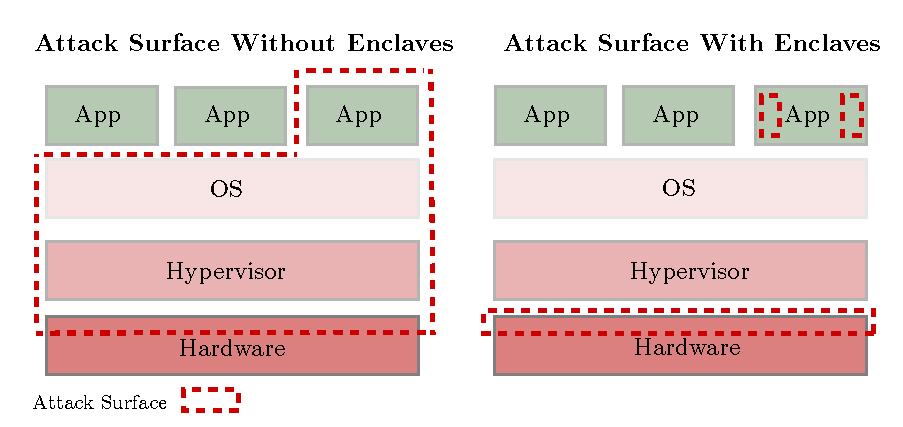
\includegraphics[width=\textwidth]{enclave}
	\caption{
		Attack surface with \acrshort{tee}.
		Adapted from \url{sgx101.gitbook.io}.
	}%
	\label{figure:enclave}
\end{figure}


		While \acrshort{tee} is a concept defining an execution environment, specific solutions include a hardware security module (a plug-in device with a protected memory and a crypto-optimized processing unit), an \acrshort{fpga}, and a set of extensions to an existing processor architecture, such as an \acrshort{sgx} for Intel x86 or Secure Encrypted Virtualization \cite{amd-memory-encryption} for AMD\@.
		Of all these, Intel \acrshort{sgx} is the most widely used technology.

		\subsection{\texorpdfstring{\acrlong{sgx}}{Software Guard Extensions}}

			\acrfull{sgx} is a set of instructions for the Intel x86 architecture that allow a user or an \acrlong{os} to define a region of protected memory, called the \emph{enclave}, and interact with it.
			The enclave can only be accessed using the \acrshort{sgx} instructions (i.e, regular \texttt{mov} instruction would not work), and all pages of the enclave are symmetrically encrypted and physically protected.
			\acrshort{sgx} guarantees the integrity and security of the memory pages within the enclave.
			Although the size of enclave memory is very limited, \acrshort{sgx} can use regular \acrshort{ram} by transparently swapping the pages between the trusted and untrusted memory.
			The pages are then encrypted with integrity protection when placed in the \acrshort{ram} (\emph{sealing} in \acrshort{sgx} terms).

			An \acrshort{sgx}-enabled application declares its trusted and untrusted components upfront.
			Trusted part will live entirely in the enclave, while the untrusted part is a normal process that runs within the \acrshort{os}.
			The application has to be digitally signed for the enclave to accept it, and the enclave itself can authenticate to the user via an \emph{attestation} process.
			Conceptually, the simplest \acrshort{sgx} application in an outsourced database system can be seen as a trusted component that operates over sensitive material (e.g., keys, tokens, plaintext user data), a remote trusted client application that communicates with the enclave, and a layer of code that passes requests through (untrusted part of an \acrshort{sgx} application).
			Cipherbase \cite{cipherbase-daas} and StealthDB \cite{stealth-db} are good examples of such approach.

		\subsection{Issues with \acrshort{sgx}}

			\acrshort{sgx}, as the closest instantiation of \acrshort{tee} available, has been extensively targeted.
			The attacks include Foreshadow \cite{foreshadow}, Prime+Probe cache attack \cite{prime-probe-sgx-attack}, an attack from within the enclave \cite{enclave-sgx-attack}, Spectre line of attacks that can bypass \acrshort{sgx} \cite{spectre-sgx-attack}, replay attack \cite{replay-sgx-attack}, Plundervolt attack \cite{plundervolt-sgx-attack}, Load Value Injection attack \cite{lvi-sgx-attack} and SGAxe attack \cite{sgaxe-sgx-attack}.
			Due to its many security issues, \acrshort{sgx} has been officially discontinued.\footnote{As of $11^\text{th}$ Generation Intel Core processor.}

			Besides the attacks against the \acrshort{sgx}, the design itself has a number of restrictions.
			First of all, the enclave memory is capped at \SI{128}{\mega\byte}, part of which is occupied by the \acrshort{sgx} control structures, leaving the application about \SI{96}{\mega\byte}.
			\acrshort{sgx} allows the use of external memory pages through the sealing mechanism, but it imposes high overhead of re-encryption and crossing the enclave physical boundary.
			Second, the code execution inside the enclave is significantly slower.
			Third, by design, only the untrusted application component can interact with the \acrshort{os}, for example, make network or storage \acrshort{io} requests.
			Finally, from the security standpoint the enclave is vulnerable against the side-channel attacks, most of all, access pattern leakage.
			Such leakage implies that the normal database application cannot be placed directly in the enclave and be deemed secure, because access pattern has been effectively exploited up to a reconstruction attack \cite{generic-attacks-kellaris}.
			One then has to design the application specifically to conceal the access pattern.
			For example, ZeroTrace \cite{zerotrace} is a variant of PathORAM \cite{path-oram} that is internally oblivious and thus can work in \acrshort{sgx}.
			Oblix \cite{oblix} is another example of a structure that is, in \textcite{oblix} own terms, doubly-oblivious --- internally in how manages memory and registers, and externally in how it interacts with a storage.

	\cleardoublepage%
	\chapter{Related work}\label{section:related-work}
\thispagestyle{myheadings}

	\section{Privacy}

		\subsection{$k$-anonymity}

		\subsection{$l$-diversity}

		\subsection{$t$-closeness}

		\subsection{\texorpdfstring{\acrlong{dp}}{Differential Privacy}}

	\section{Range query security in a snapshot model}

		\subsection{Property-Preserving Encryption}

		\subsection{\texorpdfstring{\acrlong{sse}}{Searchable Symmetric Encryption}}

		\subsection{Fully Homomorphic Encryption}

		\subsection{Attacks}

	\section{Range query security in a persistent model}

		\subsection{\texorpdfstring{\acrlong{ap}}{Access Pattern}}

		\subsection{\texorpdfstring{\acrlong{cv}}{Communication Volume}}

		\subsection{\texorpdfstring{\acrlong{tee}}{Trusted Execution Environment}}

		\subsection{Attacks}

	\section{\texorpdfstring{\acrshort{knn}}{kNN} query security in a snapshot model}

		\subsection{Attacks}

	\cleardoublepage%
	\chapter{Range queries in the persistent model}
\thispagestyle{myheadings}

	There are plenty of works offering range query solutions in a snapshot adversary model.
	Some authors propose a new \acrfull{ore} scheme to be used inside an existing range query index, see \cite{bclo-ope,clww-ore,lewi-wu-ore,cloz-ore,fh-ope}.
	Others suggest complete client-server protocols with different security guarantees, see \cite{florian-protocol,pope,practical-ore}.

	Instead of adding another solution to the mix, we developed a robust evaluation framework to compare and audit different \acrshort{ore} schemes and range query protocols \cite{ore-benchmark-17}.
	We have noticed that all proposed solutions offer their own formal protocol, security definition (which they obliviously satisfy), and even performance metrics.
	Moreover, only a few of these algorithms have ready-to-use open-sourced code.
	More often, the implementation is a prototype (or does not even exist), rendering experiments non-reproducible.

	Our work addresses these shortcomings.
	We proposed a common framework where all analyzed solutions follow the same formal protocol, a variant of an outsourced database from \cref{section:proposal:intro:model}.
	The schemes and protocols are also tested against the same security definition, a variant of a simulation-based security game where the simulator has a leakage function that is different for each solution.
	Lastly, all protocols are implemented in the same language and runtime, and are using the same cryptographic primitive implementations.

	We have paid extra attention to how we quantify the performance.
	Published works typically claim that they have implemented the algorithm in some language and ran it on a server many times measuring the wall-clock time.
	Such metric is deeply flawed since it only measures just that --- the wall-clock time it took for a particular machine to execute a particular code that references particular implementations of primitives and makes (or even does not make) \acrshort{io} requests to particular hardware.
	What we offer is a metric that drops all these ``particulars'' (i.e., dependencies) from the protocol execution.
	On top of having all solutions implemented in the same language and using the same primitives, instead of measuring the time we count the number of times an \acrshort{ore} scheme makes use of a primitive and a protocol makes an \acrshort{io} request.
	This metric is much more demonstrative: one can always get a wall-clock time estimate given these counts and the specs of the hardware.
	Moreover, we can analyze these counts theoretically from the pseudocode and then verify them practically after running the code.

	\section{\acrshort{ope} and \acrshort{ore} schemes}

		One of the ways to run a range query in the presence of a snapshot adversary is to use a conventional database range index, such as \BPlus{} tree~\cite{b-tree}, and encrypt the values in the index in a way that preserves their comparison result.
		This is exactly what \gls{ope} does.
		\gls{ope} is a scheme, a tuple of algorithms \algo{OPE.KeyGen}, \algo{OPE.Enc} and \algo{OPE.Dec}, that generate a kay, encrypt and decrypt a number respectively with a property that if $x$ was smaller, greater or equal to $y$, then their respective ciphertexts will maintain the relation.
		\gls{ore} works similarly except that the ciphertexts are not necessarily numbers and a comparison is an explicit algorithm \algo{ORE.Cmp} over hte ciphertexts.
		Formally, \gls{ope} is a specific \gls{ore} where ciphertexts are numbers and comparison is trivial, therefore, in this work I will only refer to \gls{ore}.

		Security of an \gls{ore} scheme is typically defined as via security game and a leakage profile \cite{practical-ore}.
		The scheme is defined secure with a leakage \leakage{} if there exists a simulator that can use the leakage function and can generate output indistinguishable from the one generated by the real scheme \cite{ore-benchmark-17}.
		The leakage function, ranging from as much as half of the bits of input to as little as an equality pattern of the most-significant differing bit of two inputs, is the defining security level of a scheme.

		In the comparative evaluation work \cite{ore-benchmark-17}, I choose five \gls{ore} scheme and analyze them under common framework.
		Below I concisely describe the schemes and give a summary of my finding in \cref{table:ore}.

		\subsection{BCLO}

			\cite{bclo-ope} has in its core the natural connection between a random order-preserving function and the \gls{hg}.
			The encryption algorithm is simple: split the domain into parts according to a sample from \gls{hg}, and split the range recursively and stop when the domain has one element.
			To decrypt, do the same ``path'' of splitting using the same randomness.
			The leakage if this scheme is approximately the square root of the domain, or half of the input bits.

		\subsection{CLWW}

			\cite{practical-ore} splits the inputs into $n$ sub-strings, starting with the most significant bits.
			The substring is then supplied to a keyed \gls{prf} and added to the next less significant bit.
			The comparison can then go over the two lists in-order and exit when one element is greater than the other by one.
			Naturally, the scheme leaks the location of the first differing bit.

		\subsection{Lewi-Wu}

			\cite{lewi-wu-ore} builds on \cite{practical-ore} but encrypts the input block-wise.
			For each block, left and right ciphertexts get generated, and the comparison is defined for the left part of one and the right part of the other ciphertext.
			Inside the block the bits are permuted such that one side has all permutations encoded and the other one has the correct comparison.
			This scheme reveals the location of the first differing block, but hides the differing bit inside it.

		\subsection{CLOZ}

			\cite{adam-ore-v2} also builds on \cite{practical-ore} but permutes the list of \gls{prf} outputs.
			\textcite{adam-ore-v2} observe that knowing the order is not necessary as one can compare each element of one list with every element of the other.
			Adversary can then count how many elements two lists have in common, and to eliminate this leakage, \textcite{adam-ore-v2} introduce a \gls{pph}.
			\gls{pph} only exposes a single predicate, in this case, $y \overset{?}{=} x + 1$, whether the difference of two values is one.
			This scheme by design hides the location of differing bit and  only reveals the quality pattern --- whether $m_2$ differs from $m_1$ before $m_3$ does.

		\subsection{FH-OPE}

			\cite{fh-ope} is different in that it is stateful.
			Its private state is a binary tree where the node's value is the plaintext and node's position in a tree is the ciphertext.
			While encryption and decryption is a natural binary tree operation, comparison is more involved.
			One needs to know the boundaries of the ciphertext, the maximum and minimum ciphertext values, and then the comparison is an operation on ranges.
			While the scheme does not leak anything about a particular ciphertext itself, it reveals the insertion order via tree structure, and the statefulness requirement makes it harder to use the scheme in practice.

		\section{Range query protocols}

			I include in the benchmark two baseline approaches --- a \BPlus{} tree with \gls{ore} and a \BPlus{} tree in \gls{oram}.
			The security of the former construction is that fo the underlying \gls{ore}, while the security of \gls{oram} solution is absolute in the snapshot setting since the \gls{oram} stores its records symmetrically encrypted.
			Between these baselines I add three dedicated range query solutions with varying efficiency and security, see \cref{table:range}.

			\subsection{B+ tree with \acrshort{ope}}

			\subsection{Kerschbaum}

				\cite{florian-protocol} proposes to maintain a circular array of symmetrically encrypted ciphertexts in order.
				To insert, the array is rotated on a uniformly sampled value to hide the locations of the smallest and largest elements.
				To search, the client interactively runs a binary search, requesting an element, decrypting it and deciding whether go left or right.
				While the security of this solution is superior to \BPlus{} tree with \gls{ore}, it steal leaks total order of the elements and requires full array rotation each insertion.

			\subsection{POPE}

				\cite{pope} makes an opposite trade off in efficiency to \cite{florian-protocol} --- it favors many insertions over few queries.
				\cite{pope} maintains a variant of a buffer tree, where insertion always lands an element in the root and allows lazy sorting later.
				To answer a query, the client interacts with the server to sort the buffers and split them into tree nodes.
				Once the three is structured, answering a query amounts to returning all ciphertexts between two endpoint leaves.
				\cite{pope} performance and security is different before the first query (cold) and after (warm).
				Cold unsorted buffer leaks nothing to the snapshot adversary, while warm structured tree reveals partial order.

			\subsection{Logarithmic-BRC}

				\cite{practical-range-search} uses \gls{sse} scheme and maps inputs to the ranges in which they lie.
				\gls{sse} scheme is an interactive protocol that lets the client query the document by keywords.
				\cite{practical-range-search} constructs a binary tree where each leaf is associated with one record and each intermediate node with a range so that its children are all in that range.
				Upon query, the client compute a cover --- a set of nodes that perfectly cover the requested range, and \gls{sse} scheme returns the records.
				The security of this scheme is that of the underlying \gls{sse}.

			\subsection{B+ tree in \acrshort{oram}}

	\section{Experimental Evaluation}

		In our work, we apply the framework to ten range query solutions.
		Five protocols are built with an \acrfull{ore} scheme coupled with a \BPlus{} tree.
		In \protocolSetup{}, \client{} encrypts all search keys with the \acrshort{ore} scheme, constructs a \BPlus{} tree from the ciphertexts and uploads it to \server{}.
		In \protocolQuery{}, \client{} sends encrypted query endpoints and \server{} follows standard \BPlus{} traversal.
		Such protocol leaks the total order of the records plus the leakage of the underlying \acrshort{ore} scheme.

		We also analyzed dedicated range query protocols from \cite{florian-protocol,pope,practical-range-search} and two more baselines.
		Baselines are chosen at the extremes of performance / security spectrum --- a plaintext \BPlus{} tree and a \BPlus{} tree in \acrshort{oram}.
		Intuitively, all solutions should lie between the baselines in both performance and security, but we show that at least performance-wise it is not the case (see one of the plots in \cref{figure:ore}).

		Please see \cref{table:ore,table:range} in \cref{appendix:ore-results} for the analytical results for each solution, and \cite{ore-benchmark-17} for experimental results.

		\begin{figure}[h]
	\centering
	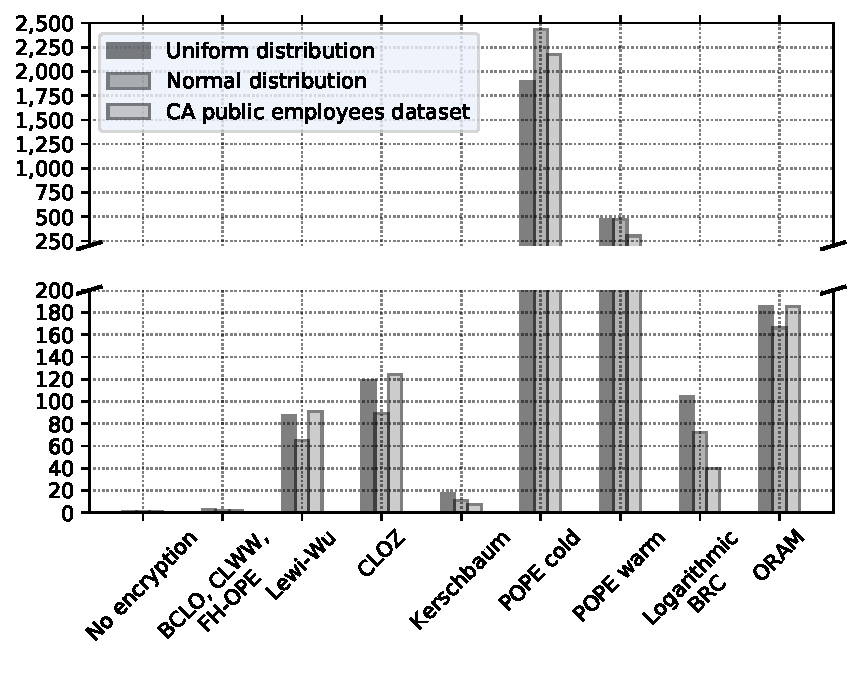
\includegraphics[width=1.0\textwidth]{protocol-charts-qios}
	\caption{Query stage number of I/O requests \cite[Figure 2d]{ore-benchmark-17}}\label{figure:ore}
\end{figure}


	\cleardoublepage%
	\chapter{Range queries in the persistent model}\label{section:range-persistent}
\thispagestyle{myheadings}

	In this section\ldots{}

	\section{Introduction}

	Secure outsourced database systems aim at helping organizations outsource their data to untrusted third parties, without compromising data confidentiality or query efficiency.
	The main idea is to encrypt the data records before uploading them to an untrusted server along with an index data structure that governs which encrypted records to retrieve for each query.
	While strong cryptographic tools can be used for this task, existing implementations such as CryptDB \cite{crypt-db}, Cipherbase \cite{cipherbase-daas}, StealthDB \cite{stealth-db} and TrustedDB \cite{trusted-db} try to optimize performance but do not provide strong security guarantees when answering queries.
	Indeed, a series of works \cite{multidimensional-range-queries, inference-attack-islam-14, leakage-abuse-attacks-cash-15, inference-attacks-naveed-15, generic-attacks-kellaris, attacks-tao-of-inference, grubbs-attacks, access-pattern-disclosure, attacks-improved-reconstruction} demonstrate that these systems are vulnerable to a variety of reconstruction attacks.
	That is, an adversary can fully reconstruct the distribution of the records over the domain of the indexed attribute.
	This weakness is prominently due to the \emph{access pattern leakage}: the adversary can tell if the same encrypted record is returned on different queries.

	More recently, \cite{generic-attacks-kellaris, state-of-uniform, attacks-improved-reconstruction, pump-volume-attacks, volume-range-attacks} showed that reconstruction attacks are possible even if the systems employ heavyweight cryptographic techniques that hide the access patterns, such as homomorphic encryption \cite{arbitrary-functions-encrypted, fully-homomorphic-encryption} or \acrfull{oram} \cite{oram-theory, oram-original}, because they leak the size of the result set of a query to the server (this is referred to as \emph{communication volume leakage}). % chktex 2
	Thus, even some recent systems that provide stronger security guarantees like ObliDB \cite{oblidb}, Opaque \cite{opaque} and Oblix \cite{oblix} are susceptible to these attacks. % chktex 2
	This also means that no outsourced database system can be both optimally efficient and privacy-preserving: secure outsourced database systems should not return the exact number of records required to answer a query.

	We take the next step towards designing secure outsourced database systems by presenting novel constructions that strike a provable balance between efficiency and privacy.
	First, to combat the access pattern leakage, we integrate a layer of \acrshort{oram} storage in our construction.
	Then, we bound the communication volume leakage by utilizing the notion of \acrfull{dp} \cite{differential-privacy-original}.
	Specifically, instead of returning the exact number of records per query, we only reveal perturbed query answer sizes by adding random encrypted records to the result so that the communication volume leakage is bounded.
	Our construction guarantees privacy of any single record in the database which is necessary in datasets with stringent privacy requirements.
	In a medical \acrshort{hipaa}-compliant setting, for example, disclosing that a patient exists in a database with a rare diagnosis correlating with age may be enough to reveal a particular individual.

	The resulting mechanism achieves the required level of privacy, but implemented na\"{\i}vely the construction is prohibitively slow.
	We make the solution practical by limiting the amount of noise and the number of network roundtrips while preserving the privacy guarantees.
	We go further and present a way to parallelize the construction, which requires adapting noise-generation algorithms to maintain differential privacy requirements.

	Using our system, we have run an extensive set of experiments over cloud machines, utilizing large datasets --- that range up to 10 million records --- and queries of different sizes, and we report our experimental results on efficiency and scalability.
	We compare against best possible solutions in terms of efficiency (conventional non-secure outsourced database systems on unencrypted data) and against an approach that provides optimal security (retrieves the full table from the cloud or runs the entire query obliviously with maximal padding).
	We report that our solution is very competitive against both baselines.
	Our performance is comparable to that of unsecured plain-text optimized database systems (like MySQL and PostgreSQL): while providing strong security and privacy guarantees, we are only 4 to 8 times slower in a typical setting.
	Compared with the optimally secure solution, a linear scan (downloading all the records), we are 18 times faster in a typical setting and even faster as database sizes scale up.

	\smallskip

	To summarize, our contributions in this work are as follows:
	\begin{itemize}
		\item
			We present a new model for a \emph{differentially private} outsourced database system, \acrshort{cdpodb}, its security definition, query types, and efficiency measures.
			In our model, the adversarial honest-but-curious server cannot see the record values, access patterns, or exact communication volume.

		\item
			We describe a novel construction, \epsolute{}, that satisfies the proposed security definition, and provide detailed algorithms for both range and point query types.
			In particular, to conceal the access pattern and communication volume leakages, we provide a secure storage construction, utilizing a combination of \acrlong{oram} \cite{oram-theory, oram-original} and differentially private sanitization \cite{non-interactive-database-privacy}.
			Towards this, we maintain an index structure to know how many and which objects we need to retrieve.
			This index can be stored locally for better efficiency (in all our experiments this is the case), but crucially, it can also be outsourced to the adversarial server and retrieved on-the-fly for each query.

		\item
			We improve our generic construction to enable parallelization within a query.
			The core idea is to split the storage among multiple \acrshortpl{oram}, but this requires tailoring the overhead required for differential privacy proportionally to the number of \acrshortpl{oram}, in order to ensure privacy.
			We present practical improvements and optimization techniques that dramatically reduce the amount of fetched noise and the number of network roundtrips.

		\item
			Finally, we provide and open-source a high-quality C++ implementation of our system.
			We have run an extensive set of experiments on both synthetic and real datasets to empirically assess the efficiency of our construction and the impact of our improvements.
			We compare our solutions to the na\"{\i}ve approach (linear scan downloading all data every query), oblivious processing and maximal padding solution (Shrinkwrap \cite{shrinkwrap}), and to a non-secure regular \acrshort{rdbms} (PostgreSQL and MySQL), and we show that our system is very competitive.
	\end{itemize}

	\subsection{Related Work}

		We group the related secure databases, engines, and indices into three categories
		\begin{enumerate*}[label={(\roman*)}]
			\item systems that are oblivious or volume-hiding and do not require \acrfull{tee},
			\item constructions that rely on \acrshort{tee} (usually, Intel \acrshort{sgx}),
			\item solutions that use property-preserving or semantically secure encryption and target primarily a snapshot adversary.
		\end{enumerate*}
		\emph{We claim that \epsolute{} is the most secure and practical range- and point-query engine in the outsourced database model, that protects both \acrfull{ap} and \acrfull{cv} using \acrlong{dp}, while not relying on \acrshort{tee}, linear scan or padding result size to the maximum.}

		\paragraph*{Obliviousness and volume-hiding without enclave}

			This category is the most relevant to \epsolute{}, wherein the systems provide either or both \acrshort{ap} and \acrshort{cv} protection without relying on \acrshort{tee}.
			\crypte{} \cite{crypte} is a recent end-to-end system executing ``\acrshort{dp} programs''.
			\crypte{} has a different model than \epsolute{} in that it assumes two non-colluding servers, an adversarial querying user (the analyst), and it uses \acrshort{dp} to protect the privacy of an individual in the database, which includes volume-hiding for aggregate queries.
			\crypte{} also does not consider oblivious execution and attacks against the \acrshort{ap}.
			Shrinkwrap \cite{shrinkwrap} (and its predecessor SMCQL \cite{smcql}) is an excellent system designed for complex queries over federated and distributed data sources.
			In Shrinkwrap, \acrshort{ap} protection is achieved by using oblivious operators (linear scan and sort) and \acrshort{cv} is concealed by adding fake records to intermediate results with \acrshort{dp}.
			Padding the result to the maximum size first and doing a linear scan over it afterwards to ``shrink'' it using \acrshort{dp}, is much more expensive than in \epsolute{}, however.
			In addition, in processing a query, the worker nodes are performing an $O(n \log{n})$ cost oblivious sorting, where $n$ is the maximum result size (whole table for range query), since they are designed to answer more general complex queries.
			SEAL \cite{seal} offers adjustable \acrshort{ap} and \acrshort{cv} leakages, up to specific bits of leakage.
			SEAL builds on top of Logarithmic-SRC \cite{practical-range-search}, splits storage into multiple \acrshortpl{oram} to adjust \acrshort{ap}, and pads results size to a power of 2 to adjust \acrshort{cv}.
			\epsolute{}, on the other hand, fully hides the \acrshort{ap} and uses \acrshort{dp} with its guarantees to pad the result size.
			PINED-RQ \cite{pined-rq} samples Laplacian noise right in the B+ tree index tree, adding fake and removing real pointers according to the sample.
			Unlike \epsolute{}, PINED-RQ allows false negatives (i.e., result records not included in the answer), and does not protect against \acrshort{ap} leakage.
			On the theoretical side, \textcite{differential-obliviousness} (followed by \textcite{differential-obliviousness-followup}) treat the \acrshort{ap} itself as something to protect with \acrshort{dp}.
			\cite{differential-obliviousness} introduces a notion of differential obliviousness that is admittedly weaker than the full obliviousness used in \epsolute{}. % chktex 2
			Most importantly, \cite{differential-obliviousness} ensures differential privacy w.r.t.~the \acrshort{oram} only, while \epsolute{} ensures \acrshort{dp} w.r.t.~the entire view of the adversary. % chktex 2

		\paragraph*{Enclave-based solutions}

			Works in this category use trusted execution environment (usually, \acrshort{sgx} enclave).
			These works are primarily concerned with the \acrshort{ap} protection for both trusted and untrusted memory, unlike \epsolute{} which also protects \acrshort{cv}.
			Cipherbase \cite{cipherbase-daas} was a pioneer introducing the idea of using \acrshort{tee} (\acrshort{fpga} at that time) to assist with \acrshort{rdbms} security.
			HardIDX \cite{hardidx} simply puts the B+ tree in the enclave, while StealthDB \cite{stealth-db} symmetrically encrypts all records and brings them in the enclave one at a time for processing.
			EnclaveDB \cite{enclave-db} assumes somewhat unrealistic \SI{192}{\giga\byte} enclave and puts the entire database in it.
			ObliDB \cite{oblidb} and Opaque \cite{opaque} assume fully oblivious enclave memory (not available as of today) and devise algorithms that use this fully trusted portion to obliviously execute common \acrshort{rdbms} operators, like filters and joins.
			Oblix \cite{oblix} provides a multimap that is oblivious both in and out of the enclave.
			HybrIDX claims protection against both \acrshort{ap} and \acrshort{cv} leakages, but unlike \epsolute{} it only obfuscates them.
			\epsolute{} offers an indistinguishability guarantee for \acrshort{ap} and a \acrshort{dp} guarantee for \acrshort{cv}, while HybrIDX hides the exact result size and only obfuscates the \acrshort{ap}.
			Lastly, Hermetic \cite{hermetic} takes on the \acrshort{sgx} side-channel attacks, including \acrshort{ap}.
			It provides oblivious primitives, however, it only offers protection against software and not physical attacks (e.g., it trusts a hypervisor to disable interrupts).

		\paragraph*{Solutions against the snapshot adversary}

			Works in this category protect against the snapshot adversary, which takes a snapshot of the data at a fixed point in time (e.g., stolen hard drive).
			We stress that \epsolute{} provides semantic security against the snapshot adversary on top of \acrshort{ap} and \acrshort{cv} protection.
			CryptDB \cite{crypt-db} is a seminal work in this direction offering computations over encrypted data.
			It has since been shown (e.g. \cite{inference-attacks-naveed-15,inference-attack-islam-14,attacks-tao-of-inference}) that the underlying property-preserving schemes allow for reconstruction attacks.
			Arx \cite{arx} provides strictly stronger security guarantees by using only semantically secure primitives.
			Seabed \cite{seabed} uses an additively symmetric homomorphic encryption scheme for aggregates and certain filter queries.
			\textcite{ppqed} offer a method to verify and apply a predicate (a junction of conditions) using garbled circuits or homomorphic encryption without revealing the predicate itself.
			SisoSPIR \cite{sisospir} presents a mechanism to build an oblivious index tree such that neither party learns the pass taken.
			See \cite{ore-benchmark-17} for a survey of range query protocols in this category. % chktex 2

	\chapter{Background}\label{section:background}
\thispagestyle{myheadings}

	In this section, I will go over the building blocks required to construct the outsourced database systems and their components that I will discuss in the next chapters.
	These prerequisites include the symmetric encryption, \acrshortpl{oram} and PathORAM \cite{path-oram} in particular, \acrlong{dp} and \acrshort{dp} sanitizers, and finally, \acrlongpl{tee}.
	\emph{Some of the following sections were paraphrased or taken verbatim from my published work \cite{ore-benchmark-17,epsolute}.}

	\section{Symmetric encryption}\label{section:background:encryption}

		Symmetric encryption scheme is a tuple of algorithms $\algo{E} = \{ \algo{KeyGen}, \algo{Enc}, \algo{Dec} \}$ with the following properties.
		$\algo{E.KeyGen} \left( \secparam \right) \to \key$ is a \emph{randomized} algorithm that on a security parameter $\secparam$ returns a key that will be used for both encryption and decryption.
		$\algo{E.Enc} \left( m \right) \to c$ is a \emph{randomized} algorithm that on a plaintext message $m \in \bin^*$ produces its ciphertext $c \in \bin^*$.
		$\algo{E.Dec} \left( c \right) \to m$ is a \emph{deterministic} algorithm that on a ciphertext $c \in \bin^*$ produces its original plaintext message $m \in \bin^*$.

		\subsection{Security}

			The security of the symmetric encryption is typically defined as the indistinguishability under a certain attack.
			The definition is structured around the game between the challenger and the adversary \adversary{}.
			The challenger fixes one of the two ``worlds'', left or right, and the adversary wins the game if she can reliably tell which world it was.

			A weaker security definition, \acrfull{ind-cpa}, intuitively, requires that the ciphertext leaks nothing about the plaintext.
			To formalize the requirement, the adversary can give the challenger a set of plaintext pairs to encrypt, and the challenger responds with a set of ciphertexts where the left or the right part was encrypted.
			The adversary can then use any (polynomial-time) algorithm over the ciphertexts and make a guess of whether the left or the right part was encrypted.
			The claim is, if there is anything that the ciphertext leaks about the plaintext, there exists an adversary who will win.
			The security claim is therefore contrapositive --- the scheme is \acrshort{ind-cpa} secure iff there is no such adversary that wins the game.

			\acrshort{ind-cpa} security is not by itself sufficient since it does not account for the decryption part of the scheme.
			There are known attacks that decrypt the plaintext (i.e., defeat the encryption) if the adversary can trigger the decryption and observe the process or the result (see padding attack \cite{padding-attack} and \acrshort{xml} encryption attack \cite{xml-break-encryption}).

			The stronger definition, \acrfull{ind-cca}, captures the decryption component.
			It extends the \acrshort{ind-cpa} game in that the adversary can now request the challenger to decrypt \emph{any} ciphertext of her choice \emph{except} the ones that the challenger himself encrypted for the adversary.
			The adversary still outputs a guess of the two worlds and wins if reliably guesses correctly.
			Note that in this game if the decryption can fail for any reason, or even if \adversary{} can observe any difference in execution for different inputs, the scheme is insecure.
			Therefore, \acrshort{ind-cca} immediately rules out the aforementioned attacks \cite{padding-attack,xml-break-encryption}.

		\subsection{Components}

			Note that for the practical purposes I define the encryption algorithm as randomized --- producing different ciphertext for the same plaintext on every invocation.
			While this is how the symmetric encryption scheme is used in applications, formally, producing the deterministic ciphertext and randomizing it are different operations.

			The randomness is produced independently, typically using a \acrfull{prg}, and is used for both secrecy and integrity (which is necessary for \acrshort{cca} security).
			After obtaining the random bits, the algorithm repeatedly uses the block cipher (formally, a \acrfull{prp}), with the number of invocations linear in the message length.
			How the randomness and the message are combined is defined by the \emph{mode of operation} and differs from one encryption scheme to another.
			Typically, the randomness comes in a form of a block, an \acrfull{iv}, filled with random bits.
			The mode of operation then defines how the blocks and the \acrshort{iv} are combined together.

			In practical systems, the ciphertext is then broken up into components, like the ciphertext material itself, the \acrshort{iv} (varies by the scheme), the version of the key, etc.
			Also note that the encryption scheme key has a maximum number of times it can be used for encryption (its \emph{operational lifetime}).

			When it comes to the real-world encryption systems, we use standardized primitives --- a block cipher (\acrshort{prp}), a \acrlong{prg} and a mode of operation.
			\acrfull{aes} \cite{aes-nist} is a \acrshort{nist}-standardized block cipher, which operates on 128-bit blocks.
			\acrshort{nist} also offers recommendations for random number generator mechanisms \cite{nist-prg-mechanism}, constructions \cite{nist-prg-constructions} and sources of entropy \cite{nist-prg-entropy}.
			Lastly, some of the commonly used modes of operation are \acrshort{cbc} and \acrshort{ctr} \cite{nist-modes} modes for general-purpose encryption, \acrshort{gcm} \cite{nist-gcm} for an authenticated encryption and \acrshort{xts} \cite{ieee-xts} for encryption of data on block-oriented devices (e.g., disks).

	\section{\texorpdfstring{\acrlong{oram}}{Oblivious Random Access Machine}}\label{section:background:oram}

		Informally, \acrfull{oram} is a mechanism that lets the users hide their access pattern to remote storage.
		An adversarial server can monitor the actual accessed locations, but she cannot tell a read from a write, the content of the block or even whether the same logical location is being referenced.
		The notion was first defined by \textcite{oram-theory} and \textcite{oram-original}.

		More formally, a $(\eta_1, \eta_2)$-\acrshort{oram} protocol is a two-party protocol between a client \client{} and a server \server{} who maintains the storage in a form of array of blocks.
		In each round, the client \client{} has input $(o, a, d)$, where $o$ is an access type (\oramRead{} or \oramWrite{}), $a$ is a storage block address and $d$ is a new data value, or $\bot$ for read operation.
		The input of \server{} is the current storage array.
		Via the protocol, the server updates the storage or returns to \user{} the data stored at the requested block, respectively.
		We speak of a sequence of such operations as a program \oramProgram{} being \emph{executed under the \acrshort{oram}}.

		An \acrshort{oram} protocol must satisfy correctness and security.
		Correctness requires that \client{} obtains the correct output of the computation except with at most probability $\eta_1$.
		For security, we require that for every client \client{} there exists a simulator $\simulator_\oram$ which provides a simulation of the server's view in the above experiment given only the number of operations.
		That is, the output distribution of $\simulator_\oram (c)$ is indistinguishable from $\algo{View}_\server$ with probability at most $\eta_2$ after $c$ protocol rounds.
		Note that the \acrshort{oram} protocols typically differ in the way the storage is organized and manipulated, but are similar in that the records or blocks are symmetrically encrypted (see \cref{section:background:encryption}).

		\acrshort{oram} protocols are generally stateful, after each execution the client and server states are updated.
		\emph{For brevity, throughout the thesis I will assume the \acrshort{oram} state updates are implicit, including the encryption key generated and maintained by the client.}

		Some existing efficient \acrshort{oram} protocols are Square Root \acrshort{oram} \cite{oram-theory}, Hierarchical \acrshort{oram} \cite{oram-original}, Binary-Tree \acrshort{oram} \cite{binary-tree-oram}, Interleave Buffer Shuffle Square Root \acrshort{oram} \cite{shortest-path-oram}, TP-ORAM \cite{tp-oram}, PathORAM \cite{path-oram} and TaORAM \cite{taostore}.
		For detailed descriptions of each protocol, I recommend the work of \textcite{oram-survey-feifei}.
		The latter three \acrshortpl{oram} achieve the lowest communication and storage overheads, $\bigO{\log \dataSize}$ and \bigO{\dataSize}, respectively.

		\subsection{PathORAM}

			PathORAM \cite{path-oram} is one of the most commonly used \acrshort{oram} protocols due to its efficiency and simplicity.
			In this section I briefly describe this construction as it is used as an \acrshort{oram} instantiation in the rest of the thesis.

			In the PathORAM, both the client \client{} and the server \server{} are stateful.
			The server stores the encrypted records (blocks) grouped in buckets, and the buckets form a binary tree.
			The client's storage, although asymptotically linear in the data size, is relatively small in practice.
			The client stores the \emph{position map} that maps the record ID to a leaf in the server tree storage and a small amount of stash, which can store some plaintext blocks on the client side.

			The main invariant of the protocol is that at all times the ciphertext of the record $a$ is stored somewhere on the \emph{path} from the root to the leaf that is mapped to $a$, or in the stash (hence the name of the construction).

			The \acrshort{oram} is initialized with a binary tree of buckets with all buckets containing valid encryptions of dummy records.
			The position map is sampled at random (filled with permuted distinct numbers).

			Main routine of the \acrshort{oram} is an access sub-protocol, which is similar for read \oramRead{} and write \oramWrite{} type of access (remember, \acrshort{oram} hides the type of access from the curious server).
			In PathORAM, the access $(o, a, d)$ consists of four steps.
			First, remap the current leaf $x$ for $a$ to a new random leaf $x^\prime$.
			Second, read the entire path to leaf $x$ (all buckets from root to leaf) into the client stash.
			Third, the client updates the block value to $d$ if the access is a write \oramWrite{}.
			Finally, write back the path to leaf $x$ filling the buckets with all blocks from stash in a way that maintains the invariant.

			The newly updated block $a$ with the new value $d$ may be included in the new path, or it may stay in the stash.
			It is important that the stash size be provably bounded.
			\cite[Theorem 1]{path-oram} does exactly that --- at least for the bucket size of 5, the probability of stash overflow and its size are related as in \cref{equation:path-oram-stash}.
			\begin{equation}\label{equation:path-oram-stash}
				\probability{ \mathsf{stash\ size} > x } \leq 14 \cdot (0.6002) ^ x
			\end{equation}
			If the probability of a protocol failure is thought of as the adversary's advantage (the probability to break the security), then the stash size equivalent to 128-bit security is about 100 blocks for the bucket of size 5 \cite[Figure 5]{path-oram}.

	\section{\texorpdfstring{\acrlong{dp}}{Differential Privacy}}

		\acrfull{dp} is a guarantee on a mechanism that takes a dataset and returns some result.
		The guarantee states that for two neighboring databases (that differ in exactly one record), the probability that the adversary will understand by looking at the output, which of the two databases was used as an input, is bounded.
		More formally, the \acrlong{dp} is defined in \cref{definition:dp}.

		\begin{definition}[\acrlong{dp}, adapted from \cite{our-data-ourselves, differential-privacy-original}]\label{definition:dp}
			A randomized algorithm \algo{A} is $(\epsilon, \delta)$-differentially private if for all $\database_1 \sim \database_2 \in \searchKeyDomain^\dataSize$, and for all subsets $\mathcal{O}$ of the output space of \algo{A},
			\[
				\probability{ \algo{A}{ \database_1 } \in \mathcal{O} } \leq \exp(\epsilon) \cdot \probability{ \algo{A}{ \database_2 } \in \mathcal{O} } + \delta \; .
			\]
		\end{definition}

		One way to interpret this definition is the following.
		Probabilities are taken over the coins of algorithm \algo{A}, which answers a query based on a dataset.
		A natural instantiation of \algo{A} is a view of a distinguishing adversary \adversary{}, who tries to guess which of the two datasets was used.
		The expression in \cref{definition:dp} then bounds the advantage of \adversary{} with $\epsilon$ and $\delta$ parameters.
		Note that $\exp( x ) \approx 1 + x + \frac{x^2}{2!}$, and for sufficiently small $x$ the last term is negligible.
		If we put $\epsilon + 1$ in place of $\exp( \epsilon )$, it becomes clear that $\epsilon$ is the exact value by which two probabilities are allowed to differ.
		For $\epsilon = 0$, they have to be equal, for $\epsilon = 0.01$, probabilities may differ by \SI{1}{\percent}.
		Therefore, $\epsilon$ is called \emph{a privacy budget} of a \acrshort{dp} system.
		$\delta$ term is additive and therefore must be small by itself.
		This term is essentially a probability that the entire system fails.
		For example, if \algo{A} is a randomized algorithm that fails with a certain chance, this probability will be $\delta$.
		For instance, a PathORAM \cite{path-oram} algorithm can have a stash overflow with a bounded probability \cite[Theorem 1]{path-oram} and it will cause the entire algorithm to fail.
		If PathORAM is used in a \acrshort{dp} system then this probability, however small, bounded and negligible, will have to be accounted for in $\delta$.

		Note that \cref{definition:dp} describes a property of \algo{A} and not a construction method.
		To construct \algo{A}, the seminal work of \textcite{differential-privacy-original} offers an algorithm called \acrfull{lpa}.
		The idea is to tune the noise sampled from the Laplacian distribution to the \emph{sensitivity} of a query, defined as the change of output with respect to change in input.
		For example, if a change in one record of the dataset causes a change in the output value of at most one (e.g., a count query), then the sensitivity is 1.
		\cite{differential-privacy-original} proves that if one adds $\algo{Laplace}{0, \frac{\mathsf{sensitivity}}{\epsilon}}$ to the real result of a query, the resulting mechanism is $\epsilon$-\acrshort{dp}.

		\subsection{\texorpdfstring{\acrshort{dp}}{DP} sanitizers}\label{section:background:dp-sanitizers}

			While the \acrlong{lpa} is an effective and simple way of answering a single count query, we will need to answer a sequence of count queries, ideally, without imposing a bound on the length of this sequence.
			We will hence make use of \emph{sanitization} algorithms.

			\begin{definition}\label{definition:dp-danitizer}
				Let \querySet{} be a collection of queries.
				An $(\epsilon, \delta, \alpha, \beta)$-differentially private sanitizer for \querySet{} is a pair of algorithms $(\algo{A}, \algo{B})$ such that:
				\begin{itemize}
					\item $A$ is $(\epsilon, \delta)$-differentially private, and
					\item on input a dataset $\database = \fromNtoM{d}{1}{\dataSize} \in \searchKeyDomain^\dataSize$, \algo{A} outputs a data structure \serverDS{} such that with probability $1 - \beta$ for all $\query \in \querySet$, $\abs{ \algo{B}{ \serverDS, \query } - \sum_i \query(d_i) } \leq \alpha$.
				\end{itemize}
			\end{definition}

			In \cref{definition:dp-danitizer}, the query is a predicate, which is defined as in \cref{section:introduction:model:odb}, and it returns a scalar 0 or 1 when executed over a search key (an attribute) $d \in \searchKeyDomain$.
			$\algo{B}{ \serverDS, \query }$ then returns a count, a scalar value which bounds the number of search keys that satisfy the query.
			For example, a query \query{} can be a range query, then $ \sum_i \query(d_i) $ is the number of records in the range, and $ \algo{B}{ \serverDS, \query } $ returns a scalar value of noise (the fake records), such that it is within $\alpha$ from the true count.

			\begin{remark}\label{remark:dp-sanitizer-guarantees}
				Given an $(\epsilon, \delta, \alpha, \beta)$-\acrshort{dp} sanitizer as in \cref{definition:dp-danitizer} one can replace the answer $\algo{B}{ \serverDS, \query }$ with $\textsc{B}^\prime ( \serverDS, \allowbreak \query ) = \algo{B}{ \serverDS, \query } + \alpha$.
				Hence, with probability $1 - \beta$, for all $\query \in \querySet$, $0 \leq \algo{\ensuremath{\textsc{B}^\prime}}{ \serverDS, \query } - \sum_i \query(d_i) \leq 2 \alpha$.
				We will hence assume from now on that sanitizers have this latter guarantee on their error.
			\end{remark}

			The main idea of \emph{sanitization} (a.k.a.\ private data release) is to release specific noisy statistics on a private dataset once, which can then be combined in order to answer an arbitrary number of queries without violating privacy.
			Depending on the query type (see \cref{section:intro:model:query-types}) and the notion of differential privacy (i.e., pure or approximate), different upper bounds on the error have been proven.
			Omitting the dependency on $\epsilon, \delta$, in case of point queries over domain size \domainSize{}, pure differential privacy results in $\alpha = \bigTheta{\log \domainSize}$ \cite{bounds-on-sample-complexity}, while for approximate differential privacy $\alpha = \bigO{1}$ \cite{private-learning-and-sanitization}.
			Note that the sanitizers add noise to a count of records, and for the point queries the count is the number of records with a given categorical value (i.e., number of female students in a class).
			For range queries over domain size \domainSize{}, these bounds are $\alpha = \bigTheta{\log \domainSize}$ for pure differential privacy \cite{non-interactive-database-privacy,dp-under-observation}, and $\alpha = \bigO{(\log^{*} \domainSize)^{1.5}}$ for approximate differential privacy (with an almost matching lower bound of $\alpha = \bigOmega{\log^{*} \domainSize}$) \cite{private-learning-and-sanitization, dp-release, privately-learning-thresholds}.
			More generally, \textcite{non-interactive-database-privacy} showed that any finite query set \querySet{} can be sanitized, albeit non-efficiently.

			\subsubsection{Answering point and range queries with differential privacy}

				Utilizing the \acrshort{lpa} for answering point queries results in error $\alpha = \bigO{\log \domainSize}$.
				A practical solution for answering range queries with error bounds very close to the optimal ones is the hierarchical method \cite{dp-under-observation, accuracy-dp-histograms, dp-wavelet}.
				The main idea is to build an aggregate tree on the domain, and add noise to each node proportional to the tree height (i.e., noise scale logarithmic in the domain size \domainSize{}).
				Then, every range query is answered using the minimum number of tree nodes.
				\textcite{hierarchical-methods-for-dp} showed that the hierarchical algorithm of \textcite{accuracy-dp-histograms}, when combined with their proposed optimizations, offers the lowest error.

			\subsubsection{Composition}

				Finally, in this thesis I will make use of a \emph{composition} theorem (adapted from \cite{privacy-integrated-queries}) based on \cite{differential-privacy-original,our-data-ourselves}. % chktex 2
				It concerns executions of multiple differentially private mechanisms on non-disjoint and disjoint inputs.

				\begin{theorem}\label{theorem:composition}
					Let \fromNtoM{\algo{A}}{1}{r} be mechanisms, such that each $\algo{A}_i$ provides $\epsilon_i$-differential privacy.
					Let \fromNtoM{\database}{1}{r} be pairwise non-disjoint (resp., disjoint) datasets.
					Let $\algo{A}$ be another mechanism that executes $\algo{A}_1(\database_1), \ldots, \algo{A}_r(\database_r)$ using independent randomness for each $\algo{A}_i$, and returns their outputs.
					Then, mechanism $\algo{A}$ is $\left( \sum_{i=1}^r \epsilon_i \right)$-differentially private (resp., $\left( \max_{i=1}^r \epsilon_i \right)$-differentially private).
				\end{theorem}

	\section{\texorpdfstring{\acrlongpl{tee}}{Trusted Execution Environments}}

		\acrlongpl{tee} is a generalized term for a ``protected'' part of a processing engine.
		Security in this setting means a combination of confidentiality, integrity, secrecy, isolation and protection against side-channel attacks.
		\acrshort{tee} cannot be entered through system calls, jumps or register manipulations.
		Environment's memory content and integrity are protected, and neither \acrshort{os}, nor a hypervisor can access it.
		Main purpose of the \acrshort{tee} is to vastly reduce the attack surface, see \cref{figure:enclave}.

		\begin{figure}[!ht]
	\centering
	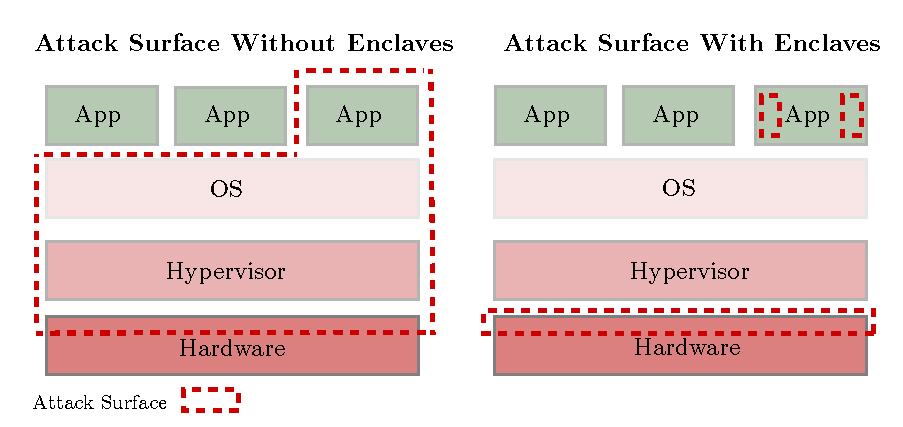
\includegraphics[width=\textwidth]{enclave}
	\caption{
		Attack surface with \acrshort{tee}.
		Adapted from \url{sgx101.gitbook.io}.
	}%
	\label{figure:enclave}
\end{figure}


		While \acrshort{tee} is a concept defining an execution environment, specific solutions include a hardware security module (a plug-in device with a protected memory and a crypto-optimized processing unit), an \acrshort{fpga}, and a set of extensions to an existing processor architecture, such as an \acrshort{sgx} for Intel x86 or Secure Encrypted Virtualization \cite{amd-memory-encryption} for AMD\@.
		Of all these, Intel \acrshort{sgx} is the most widely used technology.

		\subsection{\texorpdfstring{\acrlong{sgx}}{Software Guard Extensions}}

			\acrfull{sgx} is a set of instructions for the Intel x86 architecture that allow a user or an \acrlong{os} to define a region of protected memory, called the \emph{enclave}, and interact with it.
			The enclave can only be accessed using the \acrshort{sgx} instructions (i.e, regular \texttt{mov} instruction would not work), and all pages of the enclave are symmetrically encrypted and physically protected.
			\acrshort{sgx} guarantees the integrity and security of the memory pages within the enclave.
			Although the size of enclave memory is very limited, \acrshort{sgx} can use regular \acrshort{ram} by transparently swapping the pages between the trusted and untrusted memory.
			The pages are then encrypted with integrity protection when placed in the \acrshort{ram} (\emph{sealing} in \acrshort{sgx} terms).

			An \acrshort{sgx}-enabled application declares its trusted and untrusted components upfront.
			Trusted part will live entirely in the enclave, while the untrusted part is a normal process that runs within the \acrshort{os}.
			The application has to be digitally signed for the enclave to accept it, and the enclave itself can authenticate to the user via an \emph{attestation} process.
			Conceptually, the simplest \acrshort{sgx} application in an outsourced database system can be seen as a trusted component that operates over sensitive material (e.g., keys, tokens, plaintext user data), a remote trusted client application that communicates with the enclave, and a layer of code that passes requests through (untrusted part of an \acrshort{sgx} application).
			Cipherbase \cite{cipherbase-daas} and StealthDB \cite{stealth-db} are good examples of such approach.

		\subsection{Issues with \acrshort{sgx}}

			\acrshort{sgx}, as the closest instantiation of \acrshort{tee} available, has been extensively targeted.
			The attacks include Foreshadow \cite{foreshadow}, Prime+Probe cache attack \cite{prime-probe-sgx-attack}, an attack from within the enclave \cite{enclave-sgx-attack}, Spectre line of attacks that can bypass \acrshort{sgx} \cite{spectre-sgx-attack}, replay attack \cite{replay-sgx-attack}, Plundervolt attack \cite{plundervolt-sgx-attack}, Load Value Injection attack \cite{lvi-sgx-attack} and SGAxe attack \cite{sgaxe-sgx-attack}.
			Due to its many security issues, \acrshort{sgx} has been officially discontinued.\footnote{As of $11^\text{th}$ Generation Intel Core processor.}

			Besides the attacks against the \acrshort{sgx}, the design itself has a number of restrictions.
			First of all, the enclave memory is capped at \SI{128}{\mega\byte}, part of which is occupied by the \acrshort{sgx} control structures, leaving the application about \SI{96}{\mega\byte}.
			\acrshort{sgx} allows the use of external memory pages through the sealing mechanism, but it imposes high overhead of re-encryption and crossing the enclave physical boundary.
			Second, the code execution inside the enclave is significantly slower.
			Third, by design, only the untrusted application component can interact with the \acrshort{os}, for example, make network or storage \acrshort{io} requests.
			Finally, from the security standpoint the enclave is vulnerable against the side-channel attacks, most of all, access pattern leakage.
			Such leakage implies that the normal database application cannot be placed directly in the enclave and be deemed secure, because access pattern has been effectively exploited up to a reconstruction attack \cite{generic-attacks-kellaris}.
			One then has to design the application specifically to conceal the access pattern.
			For example, ZeroTrace \cite{zerotrace} is a variant of PathORAM \cite{path-oram} that is internally oblivious and thus can work in \acrshort{sgx}.
			Oblix \cite{oblix} is another example of a structure that is, in \textcite{oblix} own terms, doubly-oblivious --- internally in how manages memory and registers, and externally in how it interacts with a storage.

	\section{Differentially private outsourced database systems}\label{section:range-persistent:dpodb}

	In this section we present our model, \emph{differentially private outsourced database system}, \acrshort{cdpodb}, its security definition, query types and efficiency measures.
	It is an extension of the outsourced database model in \cref{section:range-persistent:background}.

	\subsection{Adversarial model}\label{section:range-persistent:dpodb:adversarial-models}

		We consider an honest-but-curious polynomial time adversary that attempts to breach differential privacy with respect to the input database \database{}.
		We observe later in \cref{section:range-persistent:dpodb:adversarial-models:adaptive} that it is impossible to completely hide the number of records returned on each query without essentially returning all the database records on each query.
		This, in turn, means that different query sequences may be distinguished, and, furthermore, that differential privacy may not be preserved if the query sequence depends on the content of the database records.
		We hence, only require the protection of differential privacy with respect to every fixed query sequence.
		Furthermore, we relax to computational differential privacy (following \cite{computational-dp}).

		In the following definition, the notation \view{\protocol{}}{\database, \fromNtoM{\query}{1}{m}} denotes the view of the server \server{} in the execution of protocol \protocol{} in answering queries \fromNtoM{\query}{1}{m} with the underlying database \database{}.

		\begin{definition}
			We say that an outsourced database system \protocol{} is $(\epsilon, \delta)$-computationally differentially private (a.k.a.~\acrshort{cdpodb}) if for every polynomial time distinguishing adversary \adversary{}, for every neighboring databases $\database \sim \database^\prime$, and for every query sequence $\fromNtoM{\query}{1}{m} \in \querySet^m$ where $m = \mathsf{poly}(\lambda)$,

			\begin{multline*}
				\probability{\adversary \left( 1^\lambda, \view{\protocol{}}{\database, \fromNtoM{\query}{1}{m}} \right) = 1 } \leq \\
				\exp{\epsilon} \cdot \probability{\adversary \left( 1^\lambda, \view{\protocol{}}{\database^\prime, \fromNtoM{\query}{1}{m}} \right) = 1} + \delta +\negl \; ,
			\end{multline*}
			where the probability is over the randomness of the distinguishing adversary \adversary{} and the protocol \protocol{}.
		\end{definition}

	\begin{remark}[Informal]
		We note that security and differential privacy in this model imply protection against communication volume and access pattern leakages and thus prevent a range of attacks, such as \cite{leakage-abuse-attacks-cash-15,inference-attacks-naveed-15,generic-attacks-kellaris}. % chktex 2
	\end{remark}

	\subsubsection{On impossibility of adaptive queries}\label{section:range-persistent:dpodb:adversarial-models:adaptive}

		Non-adaptivity in our \acrshort{cdpodb} definition does not reflect a deficiency of our specific protocol but rather an inherent source of leakage when the queries may depend on the decrypted data.
		Consider an adaptive \acrshort{cdpodb} definition that does not fix the query sequence \fromNtoM{q}{1}{m} in advance but instead an arbitrary (efficient) user \user{} chooses them during the protocol execution with \server{}.
		As before, we ask that the \server{}'s view is \acrshort{dp} on neighboring databases for every such \user{}.
		We observe that this definition cannot possibly be satisfied by \emph{any} outsourced database system without unacceptable efficiency overhead.
		Note that non-adaptivity here does not imply that the client knows all the queries in advance, but rather can choose them at any time (e.g., depending on external circumstances) as long as they do not depend on true answers to prior queries.

		To see this, consider two neighboring databases $\database, \database^\prime$.
		Database \database{} has 1 record with $\mathsf{key} = 0$ and $\database^\prime$ has none.
		Furthermore, both have 50 records with $\mathsf{key} = 50$ and 100 records with $\mathsf{key} = 100$.
		User \user{} queries first for the records with $\mathsf{key} = 0$, and then if there is a record with $\mathsf{key} = 0$ it queries for the records with $\mathsf{key} = 50$, otherwise for the records with $\mathsf{key} = 100$.
		Clearly, an efficient outsourced database system cannot return nearly as many records when $\mathsf{key} = 50$ versus $\mathsf{key} = 100$ here.
		Hence, this allows distinguishing $\database, \database^\prime$ with probability almost 1.

		To give a concrete scenario, suppose neighboring medical databases differ in one record with a rare diagnosis ``Alzheimer's disease''.
		A medical professional queries the database for that diagnosis first (point query), and if there is a record, she queries the senior patients next (range query, \texttt{age $\ge$ 65}), otherwise she queries the general population (resulting in more records).
		We leave it open to meaningfully strengthen our definition while avoiding such impossibility results, and we defer the formal proof to future work.

	% chktex-file 1
% chktex-file 8
% chktex-file 21
% chktex-file 24
% chktex-file 26
% chktex-file 36
% chktex-file 37

\newlength{\setupLength}
\setlength{\setupLength}{17em}
\newlength{\queryLength}
\setlength{\queryLength}{16em}

\begin{algorithm*}[ht!]

	\begin{pcvstack}

		\procedure[linenumbering]{\protocolSetup{}}{
													\textbf{User \user}																\>																\> \textbf{Server \server}	\\
			%
			\label{algorithm:dp-oram:setup:line-2}	\pcinput{\database}																\>																\> \pcinput{\emptyset}		\\
			%
			\label{algorithm:dp-oram:setup:line-3}	\indexI \gets \algo{CreateIndex}{\database}										\>																\>							\\
			%
			\label{algorithm:dp-oram:setup:line-4}	\oramProgram = \left. (\oramWrite, \recordID_i, \record_i) \right|_{i = 1}^n	\>																\>							\\
			%
			\label{algorithm:dp-oram:setup:line-5}																					\> \sendmessageboth*[\setupLength]{\algo{ORAM}{\oramProgram}}	\>							\\
			%
			\label{algorithm:dp-oram:setup:line-6}	\serverDS \gets \algo{A}{\fromNtoM{\searchKey}{1}{\domainSize}}					\> \sendmessageright*[\setupLength]{\serverDS}					\>							\\
			%
			\label{algorithm:dp-oram:setup:line-7}	\pcouput{\indexI}																\>																\> \pcouput{\serverDS}
		}

		\vspace{0.5em}

		\procedure[linenumbering]{\protocolQuery{}}{
													\textbf{User \user}																				\>																											\> \textbf{Server \server}				\\
			%
			\label{algorithm:dp-oram:query:line-2}	\pcinput{\query, \indexI}																		\>																											\> \pcinput{\serverDS}					\\
			%
			\label{algorithm:dp-oram:query:line-3}	T \gets \algo{Lookup}{\indexI, \query}															\> \sendmessageright*[\queryLength]{\query}																	\> c \gets \algo{B}{\serverDS, \query}	\\
			%
			\label{algorithm:dp-oram:query:line-4}	\oramProgram_\mathsf{true} = \left. (\oramRead, \recordID_i, \bot) \right|_{i \in T}			\> \sendmessageleft*[\queryLength]{c}																		\>										\\
			%
			\label{algorithm:dp-oram:query:line-5}	\oramProgram_\mathsf{noise} = \left. (\oramRead, S \setminus T, \bot) \right|_{1}^{c - \abs{T}}	\>																											\>										\\
			%
			\label{algorithm:dp-oram:query:line-6}	R																								\> \sendmessageboth*[\queryLength]{\algo{ORAM}{\oramProgram_\mathsf{true} \| \oramProgram_\mathsf{noise}}}	\>										\\
			%
			\label{algorithm:dp-oram:query:line-7}	\pcouput{R}																						\>																											\>	\pcouput{\emptyset}
		}

	\end{pcvstack}

	\caption[\epsolute{} protocol]{
		\epsolute{} protocol.
		$\algo{ORAM}{\cdot}$ denotes an execution of \acrshort{oram} protocol (\cref{section:background:oram}), where \user{} plays the role of the client.
		\acrshort{oram} protocol client and server states are implicit.
		$S \setminus T$ represents a set of valid record IDs $S$ that are not in the true result set $T$.
	}%
	\label{algorithm:dp-oram}
\end{algorithm*}


	\subsection{Query types}

		In this work we are concerned with the following query types:
		\begin{description}[style=unboxed, leftmargin=0em]
			\item[Range queries]
				Here we assume a total ordering on \searchKeyDomain{}.
				A query \query{a}{b} is associated with an interval $\interval{a}{b}$ for $1 \leq a \leq b \leq \domainSize$ such that $\query{a}{b}(c) = 1$ iff $c \in \interval{a}{b}$ for all $c \in \searchKeyDomain$.
				The equivalent \acrshort{sql} query is:

				\smallskip
				\indent\texttt{SELECT * FROM table WHERE attribute BETWEEN a AND b;}
				\smallskip

			\item[Point queries]
				Here \searchKeyDomain{} is arbitrary and a query predicate \query{a} is associated with an element $a \in \searchKeyDomain$ such that $\query{a}(b) = 1$ iff $a = b$.
				In an ordered domain, point queries are degenerate range queries.
				The equivalent \acrshort{sql} query is:

				\smallskip
				\indent\texttt{SELECT * FROM table WHERE attribute = a;}

		\end{description}

	\subsection{Measuring Efficiency}

		We define two basic efficiency measures for a \acrshort{cdpodb}.
		\begin{description}[style=unboxed, leftmargin=0em]
			\item[Storage efficiency]
				is defined as the sum of the bit-lengths of the records in a database relative to the bit-length of a corresponding encrypted database.
				Specifically, we say that an outsourced database system has \emph{storage efficiency} of $(\efficiencyCoefficient, \efficiencyOffset)$ if the following holds.
				Fix any \databaseDef{} and let $n_1 = \sum_{i=1}^n \abs{r_i}$.
				Let $\server_\mathsf{state}$ be an output of \server{} on a run of \protocolSetup{} where \user{} has input \database{}, and let $n_2 = \abs{ \server_\mathsf{state} }$.
				Then $n_2 \leq \efficiencyCoefficient n_1 + \efficiencyOffset$.

			\item[Communication efficiency]
				is defined as the sum of the lengths of the records in bits whose search keys satisfy the query relative to the actual number of bits sent back as the result of a query.
				Specifically, we say that an outsourced database system has \emph{communication efficiency} of $(\efficiencyCoefficient, \efficiencyOffset)$ if the following holds.
				Fix any \query{} and \serverDS{} output by \protocolSetup{}, let \user{} and \server{} execute \protocolQuery{} where \user{} has inputs \query{}, and output $R$, and \server{} has input \serverDS{}.
				Let $m_1$ be the amount of data in bits transferred between \user{} and \server{} during the execution of \protocolQuery{}, and let $m_2 = \abs{ R }$.
				Then $m_2 \leq \efficiencyCoefficient m_1 + \efficiencyOffset$.
		\end{description}

		Note that $\efficiencyCoefficient \geq 1$ and $\efficiencyOffset \geq 0$ for both measures.
		We say that an outsourced database system is \emph{optimally storage efficient} (resp., \emph{optimally communication efficient}) if it has storage (resp., communication) efficiency of $(1, 0)$.

	\section{\texorpdfstring{\epsolute{}}{Epsolute}}\label{section:range-persistent:dp-oram}

	In this section we present a construction, \epsolute{}, that satisfies the security definition in \cref{section:range-persistent:dpodb}, detailing algorithms for both range and point query types.
	We also provide efficiency guarantees for approximate and pure \acrshort{dp} versions of \epsolute{}.

	\subsection{General construction}

		Let \querySet{} be a collection of queries.
		We are interested in building a differentially private outsourced database system for \querySet{}, called \epsolute{}.
		Our solution will use these building blocks.
		\begin{itemize}
			\item
				A $(\eta_1, \eta_2)$-\acrshort{oram} protocol \algo{ORAM}{\cdot}.
			\item
				An $(\epsilon, \delta, \alpha, \beta)$-differentially private sanitizer $(\algo{A}, \algo{B})$ for \querySet{} and negligible $\beta$, which satisfies the non-negative noise guarantee from \cref{remark:dp-sanitizer-guarantees}.
			\item
				A pair of algorithms \algo{CreateIndex} and \algo{Lookup}.
				\algo{CreateIndex} consumes \database{} and produces an index data structure \indexI{} that maps a search key \searchKey{} to a list of record \acrshortpl{id} \recordID{} corresponding to the given search key.
				\algo{Lookup} consumes \indexI{} and \query{} and returns a list $T = \fromNtoM{\recordID}{1}{{\abs{T}}}$ of record \acrshortpl{id} matching the supplied query.
		\end{itemize}

		Our protocol $\protocol = (\protocolSetup, \protocolQuery)$ of \epsolute{} works as shown in \cref{algorithm:dp-oram}.
		Hereafter, we reference lines in \cref{algorithm:dp-oram}.
		See \cref{figure:dp-oram} for a schematic description of the protocol.

		\paragraph*{Setup protocol \; \texorpdfstring{\protocolSetup{}}{}}

			Let \user{}'s input be a database \databaseDef{} (\cref{algorithm:dp-oram:setup:line-2}).
			\user{} creates an index \indexI{} mapping search keys to record \acrshortpl{id} corresponding to these keys (\cref{algorithm:dp-oram:setup:line-3}).
			\user{} sends over the records to \server{} by executing the \acrshort{oram} protocol on the specified sequence (\crefrange{algorithm:dp-oram:setup:line-4}{algorithm:dp-oram:setup:line-5}).
			\user{} generates a \acrshort{dp} structure \serverDS{} over the search keys using sanitizer \algo{A}, and sends \serverDS{} over to \server{} (\cref{algorithm:dp-oram:setup:line-6}).
			The output of \user{} is \indexI{} and of \server{} is \serverDS{}; final \acrshort{oram} states of \server{} and \user{} are implicit, including encryption key \queryKey{} (\cref{algorithm:dp-oram:setup:line-7}).

		\paragraph*{Query protocol \; \texorpdfstring{\protocolQuery{}}{}}

			\user{} starts with a query \query{} and index \indexI{}, \server{} starts with a \acrshort{dp} structure \serverDS{}.
			One can think of these inputs as outputs of \protocolSetup{} (\cref{algorithm:dp-oram:query:line-2}).
			\user{} immediately sends the query to \server{}, which uses the sanitizer \algo{B} to compute the total number of requests $c$, while \user{} uses index \indexI{} to derive the true indices of the records the query \query{} targets (\cref{algorithm:dp-oram:query:line-3}).
			\user{} receives $c$ from \server{} and prepares two \acrshort{oram} sequences: $\oramProgram_\mathsf{true}$ for real records retrieval, and $\oramProgram_\mathsf{noise}$ to pad the number of requests to $c$ to perturb the communication volume.
			$\oramProgram_\mathsf{noise}$ includes valid non-repeating record \acrshortpl{id} that are not part of the true result set $T$ (\crefrange{algorithm:dp-oram:query:line-4}{algorithm:dp-oram:query:line-5}).
			\user{} fetches the records, both real and fake, from \server{} using the \acrshort{oram} protocol (\cref{algorithm:dp-oram:query:line-6}).
			The output of \user{} is the filtered set of records requested by the query $\query{}$; final \acrshort{oram} states of \server{} and \user{} are implicit (\cref{algorithm:dp-oram:query:line-7}).

		The protocols for point and range queries only differ in sanitizer implementations, see \cref{section:range-persistent:dp-oram:point,section:range-persistent:dp-oram:range}.
		Note above that in any execution of \protocolQuery{} we have $c \geq \query(\database)$ with overwhelming probability $1 - \beta$ (by using sanitizers satisfying \cref{remark:dp-sanitizer-guarantees}), and thus the protocol is well-defined and its accuracy is $1 - \beta$.
		Also note that the \acrshort{dp} parameter $\delta$ is lower-bounded by $\beta$ because sampling negative noise, however improbable, violates privacy, and therefore the final construction is $(\epsilon, \beta)$-\acrshort{dp}.

		\begin{figure}[!ht]
	\centering
	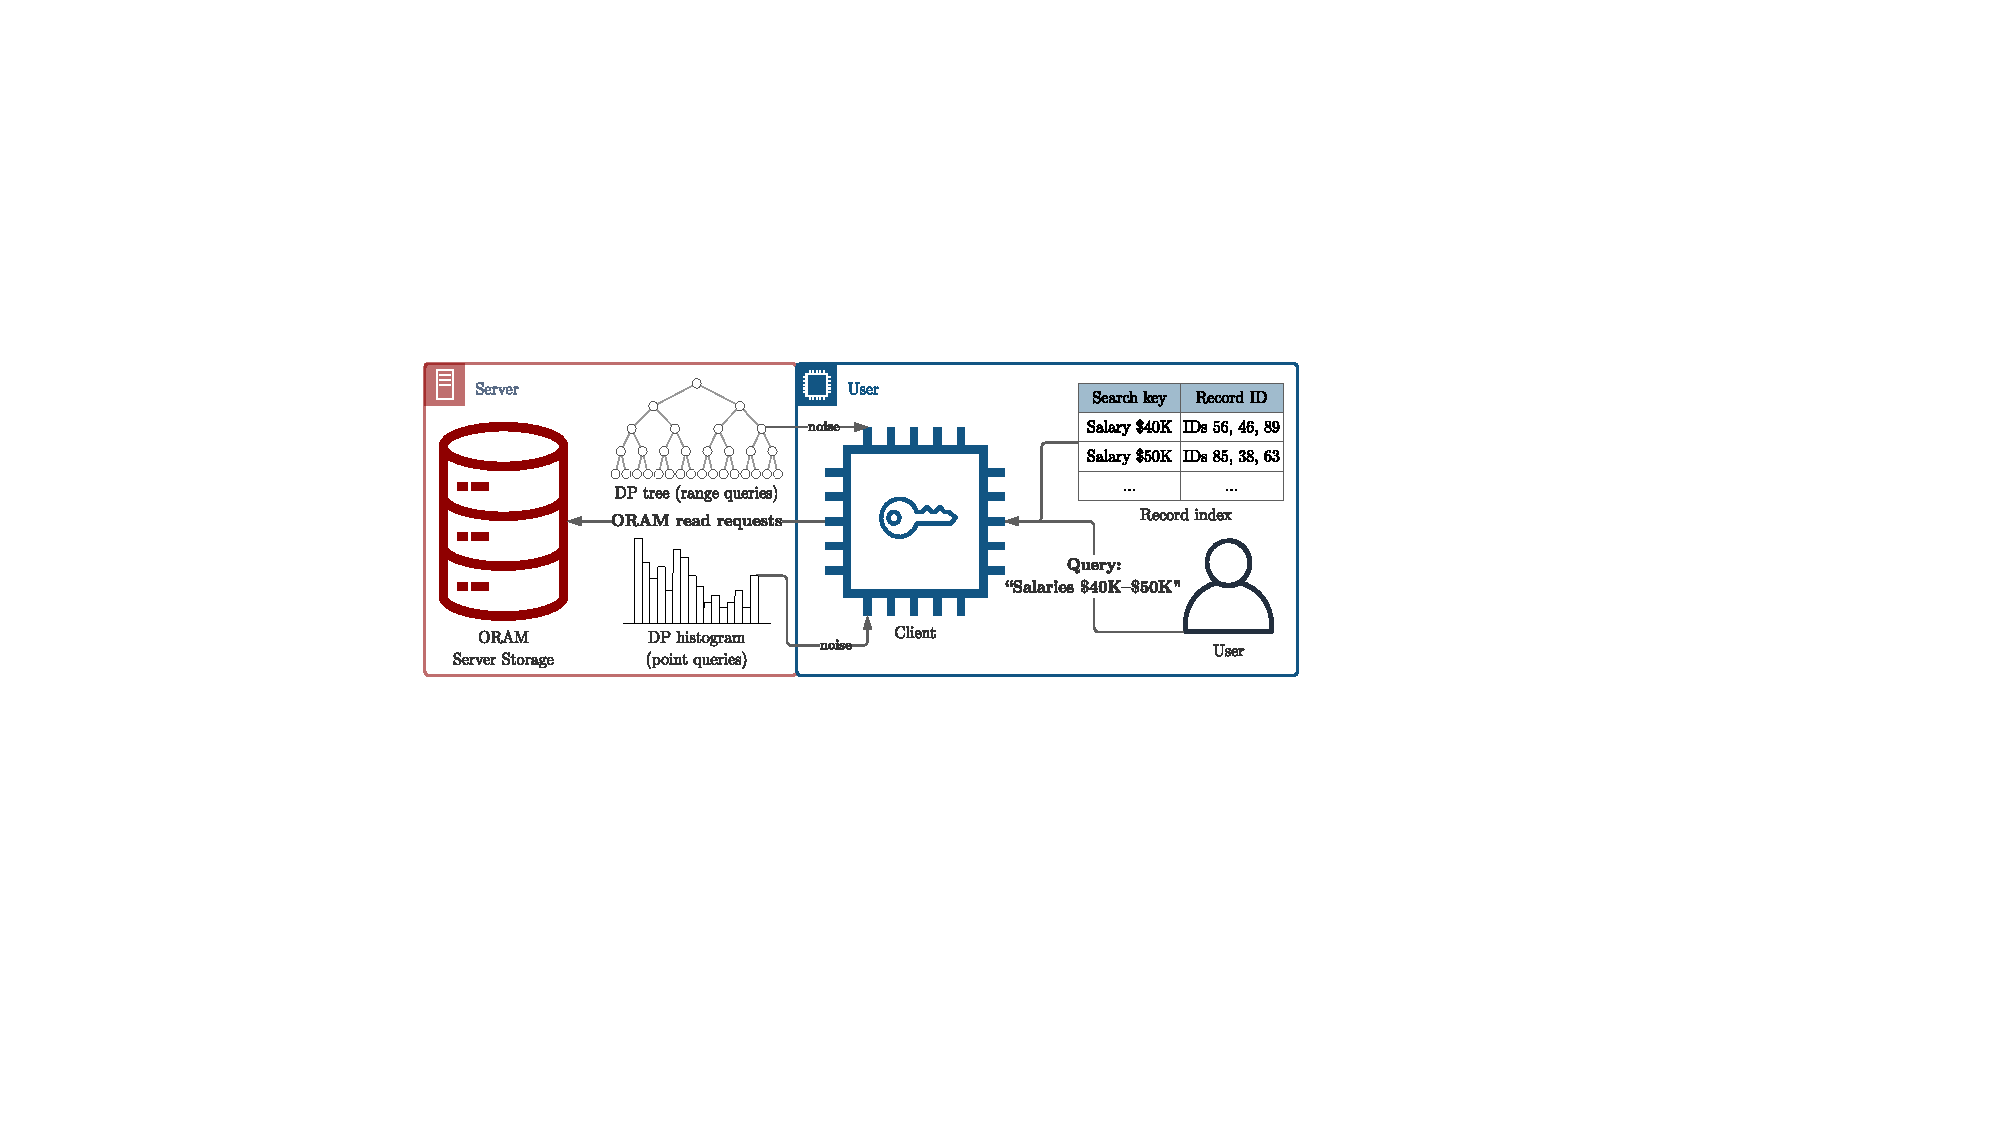
\includegraphics[width=\linewidth]{dp-oram}
	\caption{\epsolute{} construction}%
	\label{figure:dp-oram}
\end{figure}


	\subsection{Security}

		\begin{theorem}
			\epsolute{} is $(\beta \cdot m)$-wrong and $(\epsilon, \delta)$-\acrshort{cdpodb} where the negligible term is $\negl = 2 \cdot \eta_2$.
		\end{theorem}

		\begin{proof}
			We consider a sequence of views
			\[
				\view{1} \to \view{2} \to \view{3} \to \view{4} \; .
			\]
			\view{1} is \view{\protocol}{\database, \fromNtoM{\query}{1}{m}}.
			\view{2} is produced only from $\serverDS \gets \algo{A}(\fromNtoM{\searchKey}{1}{\domainSize})$. % here I explicitly use parentheses to allow line break
			Namely, compute $c_i \gets \algo{A}{\serverDS, \query_i}$ for all $i$ and run \acrshort{oram} simulator on $\sum_i c_i$.
			By \acrshort{oram} security,
			\[
				\probability{\adversary(\view{1})} - \probability{\adversary(\view{2})} \leq \eta_2 \; .
			\]
			\view{3} is produced similarly but $\serverDS \gets \algo{A}{\fromNtoM{\searchKey^\prime}{1}{\domainSize}}$ instead.
			Note that the $c_i$ are simply post-processing on \serverDS{} via \algo{B} so
			\[
				\probability{\adversary(\view{2})} = \exp(\epsilon) \cdot \probability{\adversary(\view{3})} + \delta \; .
			\]
			$\view{4} = \view{\protocol}{\database^\prime, \fromNtoM{\query}{1}{m}}$.
			It follows by \acrshort{oram} security
			\[
				\probability{\adversary(\view{3})} - \probability{\adversary(\view{4})} \leq \eta_2 \; .
			\]
			Putting this all together completes the proof.
		\end{proof}

	\subsection{Efficiency}

		For an \acrshort{oram} with communication efficiency $(a_1, a_2)$ and an $(\alpha, \beta)$-differentially private sanitizer, the \epsolute{} communication efficiency is $(a_1, a_2 \cdot \alpha)$.
		The efficiency metrics demonstrate how the total storage or communication volume (the number of stored or transferred bits) changes additively and multiplicatively as the functions of data size \dataSize{} and domain \domainSize{}.
		We therefore have the following corollaries for the efficiency of the system in the cases of approximate and pure differential privacy.
		\begin{corollary}\label{corollary:comm-efficiency-approximate-dp}
			\epsolute{} is an outsourced database system with storage efficiency \efficiency{1}{0}.
			Depending on the query type, assume it offers the following communication efficiency.
			\begin{description}
				\item[Range queries] $\efficiency{\log \dataSize}{2^{\log^* \domainSize} \log \dataSize}$
				\item[Point queries] $\efficiency{\log \dataSize}{\log \dataSize}$
			\end{description}
			Then, there is a negligible $\delta$ such that \epsolute{} satisfies $(\epsilon, \delta)$\hyp{}differential privacy for some $\epsilon$.\footnote{
				Note that the existence of $\epsilon$ in this setting implies that the probability of an adversary breaking the \acrshort{dp} guarantees is bounded by it.
			}
		\end{corollary}

		\begin{proof}
			By using \acrshort{oram}, we store only the original data once and hence, we get optimal storage efficiency.

			The communication efficiency depends on the upper bound of the error for each sanitizer when $\delta > 0$, as described in \cref{section:background:dp-sanitizers} and \cref{remark:dp-sanitizer-guarantees}.
			The most efficient \acrshort{oram} protocol to date has $\bigO{\log \dataSize}$ communication overhead (see \cref{section:background:oram}).
		\end{proof}

		\begin{corollary}\label{corollary:comm-efficiency-pure-dp}
			\epsolute{} is an outsourced database system with storage efficiency \efficiency{1}{0}.
			Depending on the query type, assume it offers the following communication efficiency.
			\begin{description}
				\item[Range queries] $\efficiency{\log \dataSize}{\log \domainSize \log \dataSize}$
				\item[Point queries] $\efficiency{\log \dataSize}{\log \domainSize \log \dataSize}$
			\end{description}
			Then, \epsolute{} satisfies $\epsilon$-differential privacy for some $\epsilon$.
		\end{corollary}

		\begin{proof}
			Similarly, we derive the proof by considering the use of \acrshort{oram} and the upper bound of the error for each sanitizer when $\delta = 0$ in \cref{section:background:dp-sanitizers}.
		\end{proof}

	\subsection{Extending to multiple attributes}\label{section:range-persistent:dp-oram:multiple-attributes}

		We will now describe how \epsolute{} supports multiple indexed attributes and what the privacy and performance implications are.
		The na\"{\i}ve way is to simply duplicate the entire stack of states of \user{} and \server{}, and during the query use the states whose attribute the query targets.
		However, \epsolute{} design allows to keep the most expensive part of the state --- the \acrshort{oram} state --- shared for all attributes and both types of queries.
		Specifically, the index \indexI{} and \acrshort{dp} structure \serverDS{} are generated per attribute and query type, while \user{} and \server{} \acrshort{oram} states are generated once.
		This design is practical since \serverDS{} is tiny and index \indexI{} is relatively small compared to \acrshort{oram} states, see \cref{section:range-persistent:experiments}.

		We note that in case the indices grow large in number, it is practical to outsource them to the adversarial server using \acrshort{oram} and download only the ones needed for each query.
		In terms of privacy, the solution is equivalent to operating different \epsolute{} instances because \acrshort{oram} hides the values of records and access patterns entirely.
		Due to \cref{theorem:composition} for non-disjoint datasets, the total privacy budget of the multi-attribute system will be the sum of individual budgets for each attribute / index.

		Next, we choose two \acrshort{dp} sanitizers for our system, for point and for range queries, and calculate the $\alpha$ values to make them output positive values with high probability, consistent with \cref{remark:dp-sanitizer-guarantees}.

	\subsection{\texorpdfstring{\epsolute{}}{Epsolute} for point queries}\label{section:range-persistent:dp-oram:point}

		For point queries, we use the \acrshort{lpa} method as the sanitizer to ensure pure differential privacy.
		Specifically, for every histogram bin, we draw noise from the Laplace distribution with mean $\alpha_p$ and scale $\lambda = \nicefrac{1}{\epsilon}$.
		To satisfy \cref{remark:dp-sanitizer-guarantees}, we have to set $\alpha_p$ such that if values are drawn from $\algo{Laplace}{ \alpha_p, \nicefrac{1}{\epsilon} }$ at least as many times as the number of bins \domainSize{}, they are all positive with high probability $1 - \beta$, for negligible $\beta$.

		We can compute the exact minimum required value of $\alpha_p$ in order to ensure drawing positive values with high probability by using the \acrshort{cdf} of the Laplace distribution.
		Specifically, $\alpha_p$ should be equal to the minimum value that satisfies the following inequality.

		\[
			\left( 1 - \frac{1}{2} e^{- \alpha_p \cdot \epsilon} \right)^\domainSize \leq 1 - \beta
		\]
		which is equivalent to
		\[
			\alpha_p = \ceil{ -\frac{ \ln \left( 2 - 2 \sqrt[\domainSize]{1 - \beta} \right) }{ \epsilon } }
		\]

	% chktex-file 1
% chktex-file 8
% chktex-file 21
% chktex-file 24
% chktex-file 26
% chktex-file 36
% chktex-file 37

\setlength{\setupLength}{16em}
\setlength{\queryLength}{15em}

\newcommand{\SetupGamma}{
	\procedure[linenumbering]{\protocolSetup{} of \protocolGamma{}}{
																\textbf{User \user}																							\>																\> \textbf{Server \server}	\\
		%
		\label{algorithm:dp-oram-parallel:gamma:setup:line-2}	\pcinput{\database{}}																						\>																\> \pcinput{\emptyset}		\\
		%
		\label{algorithm:dp-oram-parallel:gamma:setup:line-3}	\indexI \gets \algo{CreateIndex}{\database, \oramsNumber}													\>																\>							\pclb
		%
		\pcintertext[dotted]{$\pcfor j \in \set{1, \ldots, \oramsNumber} \pcdo$ \; \text{(in parallel)}}
		%
		\label{algorithm:dp-oram-parallel:gamma:setup:line-4}	\left\langle \overline{\record}, \overline{\recordID} \right\rangle\ \text{s.t.}\ \algo{H}{\recordID} = j	\>																\>							\\
		%
		\label{algorithm:dp-oram-parallel:gamma:setup:line-5}	\oramProgram = \left\langle (\oramWrite, \overline{\recordID}, \overline{\record}) \right\rangle			\> \sendmessageboth*[\setupLength]{\algo{ORAM}_j(\oramProgram)}	\>							\pclb
		%
		\pcintertext[dotted]{$\pcendfor$}
		%
		\label{algorithm:dp-oram-parallel:gamma:setup:line-6}	\serverDS \gets \algo{A}{\fromNtoM{\searchKey}{1}{\domainSize}}												\> \sendmessageright*[\setupLength]{\serverDS}					\>							\\
		%
		\label{algorithm:dp-oram-parallel:gamma:setup:line-7}	\pcouput{\indexI}																							\>																\> \pcouput{ \serverDS }
	}
}

\newcommand{\QueryGamma}{
	\procedure[linenumbering]{\protocolQuery{} of \protocolGamma{}}{
																\textbf{User \user}																					\>																												\> \textbf{Server \server}									\\
		%
		\label{algorithm:dp-oram-parallel:gamma:query:line-2}	\pcinput{\query, \indexI}																			\>																												\> \pcinput{ \serverDS }									\\
		%
		\label{algorithm:dp-oram-parallel:gamma:query:line-3}	\fromNtoM{T}{1}{\oramsNumber} \gets \algo{Lookup}{I, \query}										\> \sendmessageright*[\queryLength]{\query}																		\> k \gets \algo{B}{\serverDS, \query}						\\
		%
		\label{algorithm:dp-oram-parallel:gamma:query:line-4}																										\> \sendmessageleft*[\queryLength]{c}																			\> c \gets (1 + \gamma) \frac{\tilde{k}_0}{\oramsNumber}	\pclb
		%
		\pcintertext[dotted]{$\pcfor j \in \set{1, \ldots, \oramsNumber} \pcdo$ \; \text{(in parallel)}}
		%
		\label{algorithm:dp-oram-parallel:gamma:query:line-5}	\oramProgram_\mathsf{true} = \left. (\oramRead, \recordID_i, \bot) \right|_{i \in T_j}				\>																												\>															\\
		%
		\label{algorithm:dp-oram-parallel:gamma:query:line-6}	\oramProgram_\mathsf{noise} = \left. (\oramRead, S \setminus T_j, \bot) \right|_{1}^{c - \abs{T_j}}	\> \sendmessageboth*[\queryLength]{\algo{ORAM}_j(\oramProgram_\mathsf{true} \| \oramProgram_\mathsf{noise})}	\> R_j														\pclb
		%
		\pcintertext[dotted]{$\pcendfor$}
		%
		\label{algorithm:dp-oram-parallel:gamma:query:line-7}	\pcouput{ \left. R_j \right|_{j = 1}^\oramsNumber }													\>																												\>	\pcouput{\emptyset}
	}
}

\begin{algorithm*}[ht!]

	\begin{pcvstack}

		\begin{pcvstack}

			\SetupGamma{}

			\vspace{0.5em}

			\QueryGamma{}

		\end{pcvstack}

	\end{pcvstack}

	\caption[Parallel \epsolute{} for \protocolGamma{}]{
		Parallel \epsolute{} for \protocolGamma{}, extends \cref{algorithm:dp-oram}.
		\algo{H} is a random hash function $\algo{H} : \bin^* \to \set{1, \ldots, \oramsNumber}$.
		$\gamma$ and $\tilde{k}_0$ are computed as in \cref{section:range-persistent:prallel-dp-oram:gamma}.
	}%
	\label{algorithm:dp-oram-parallel}
\end{algorithm*}


	\subsection{\texorpdfstring{\epsolute{}}{Epsolute} for range queries}\label{section:range-persistent:dp-oram:range}

		For range queries, we implement the aggregate tree method as the sanitizer.
		Specifically, we build a complete \fanout{}-ary tree on the domain, for a given \fanout{}.
		A leaf node holds the number of records falling into each bin plus some noise.
		A parent node holds sum of the leaf values in the range covered by this node, plus noise.
		Every time a query is issued, we find the minimum number of nodes that cover the range, and determine the required number of returned records by summing these node values.
		Then, we ask the server to retrieve the records in the range, plus to retrieve multiple random records so that the total number of retrieved records matches the required number of returned records.

		The noise per node is drawn from the Laplace distribution with mean $\alpha_h$ and scale $\lambda = \frac{\log_{\fanout} \domainSize}{\epsilon}$.
		Consistent with \cref{remark:dp-sanitizer-guarantees}, we determine the mean value $\alpha_h$ in order to avoid drawing negative values with high probability.
		We have to set $\alpha_h$ such that if values are drawn from $\algo{Laplace}{ \alpha_h, \frac{\log_{\fanout} \domainSize}{\epsilon} }$ at least as many times as the number of nodes in the tree, they are all positive with high probability $1 - \beta$, for negligible $\beta$.

		Again, we can compute the exact minimum required value of $\alpha_h$ in order to ensure drawing positive values with high probability by using the \acrshort{cdf} of the Laplace distribution.
		Specifically, $\alpha_h$ should be equal to the minimum value that satisfies the following inequality.
		\[
			\left( 1 - \frac{1}{2} e^{- \frac{\alpha_h \cdot \epsilon}{\log_{\fanout} \domainSize}} \right)^\mathsf{nodes} \leq 1 - \beta
		\]
		which is equivalent to
		\begin{equation}\label{equation:min-mu-for-range}
			\alpha_h = \ceil{ -\frac{ \ln{ (2 - 2 \sqrt[\mathsf{nodes}]{ 1 - \beta } ) } \cdot \log_{\fanout} \domainSize }{\epsilon} }
		\end{equation}
		where $\mathsf{nodes} = \frac{ \fanout^{ \ceil{ \log_{\fanout} (\fanout - 1) + \log_{\fanout} \domainSize - 1 }} - 1}{ \fanout - 1 } + \domainSize$ is the total number of tree nodes.

	\section{An efficient Parallel \texorpdfstring{\epsolute{}}{Epsolute}}\label{section:range-persistent:prallel-dp-oram}

	While the previously described scheme is a secure and correct \acrshort{cdpodb}, a single-threaded implementation may be prohibitively slow in practice.
	To bring the performance closer to real-world requirements, we need to be able to scale the algorithm horizontally.
	In this section, we describe an upgrade of \epsolute{} --- a scalable parallel solution.

	We suggest two variants of parallel \epsolute{} protocol.
	Both of them work by operating \oramsNumber{} \acrshortpl{oram} and randomly assigning to each of them $\nicefrac{n}{\oramsNumber}$ database records.
	For each query, we utilize the index \indexI{} to find the required records from the corresponding \acrshortpl{oram}.
	For each \acrshort{oram}, we execute a separate thread to retrieve the records.
	The threads work in parallel and there is no need for locking, since each \acrshort{oram} works independently from the rest.
	We present two methods that differ in the way they build and store \acrshort{dp} structure \serverDS{}, and hence the number of \acrshort{oram} requests they make.

	\subsection{\texorpdfstring{No-$\gamma$-method}{No-gamma-method}: \acrshort{dp} structure per \acrshort{oram}}

		In \protocolNoGamma{}, for each \acrshort{oram} / subset of the dataset, we build a \acrshort{dp} index the same way as described in \cref{section:range-persistent:dp-oram}.
		We note that \cref{theorem:composition} for disjoint datasets applies to this construction: the privacy budget $\epsilon$ for the construction is the largest (least private) among the $\epsilon$'s of the \acrshort{dp} indices for each \acrshort{oram} / subset of the dataset.

		The communication efficiency changes because
		\begin{enumerate*}[label={(\roman*)}]
			\item
				we essentially add \oramsNumber{} record subsets in order to answer a query, each having at most $\alpha$ extra random records, and
			\item
				each \acrshort{oram} holds fewer records than before, resulting in a tree of height $\log \frac{\dataSize}{\oramsNumber}$.
		\end{enumerate*}

		However, we cannot expect that the records required for each query are equally distributed among the different \acrshortpl{oram} in order to reduce the multiplicative communication cost from $\log \dataSize$ to $\frac{\log \dataSize}{\oramsNumber}$.
		Instead, we need to bound the worst case scenario which is represented by the maximum number of records from any \acrshort{oram} that is required to answer a query.
		This can be computed as follows.

		Let $X_j$ be $1$ if a record for answering query \query{} is in a specific $\algo{ORAM}_j$, and $0$ otherwise.
		Due to the random assignment of records to \acrshortpl{oram}, $\probability{X_j = 1} = \nicefrac{1}{\oramsNumber}$.
		Assume that we need $k_0$ records in order to answer query \query{}.
		The maximum number of records from $\algo{ORAM}_j$ in order to answer \query{} is bounded as follows.

		\begin{equation}\label{equation:gamma}
			\probability{ \sum_{i=1}^{k_0} X_i > ( 1 + \gamma ) \frac{k_0}{\oramsNumber} } \leq \exp{ \left( - \frac{ k_0 \gamma^2 }{ 3 \oramsNumber } \right) }
		\end{equation}

		Finally, we need to determine the value of $\gamma$ such that $\exp{ \left( - \frac{ k_0 \gamma^2 }{ 3 \oramsNumber } \right) }$ is smaller than the value $\beta$.
		Thus, $\gamma = \sqrt{ \frac{-3 \oramsNumber \log \beta}{ k_0 } }$.
		The communication efficiency for each query type is described in the following corollary.

		\begin{corollary}\label{corollary:no-gamma}
			Let \protocolNoGamma{} be an outsourced database system with storage efficiency \efficiency{1}{0}.
			Depending on the query type, \protocolNoGamma{} offers the following communication efficiency.
			\begin{description}
				\item[Range queries] $\efficiency{\left( 1 + \sqrt{ \frac{- 3 \oramsNumber \log \beta}{k_0} } \right) \log \frac{\dataSize}{\oramsNumber} }{ \frac{ \log^{1.5} \domainSize}{ \epsilon } \oramsNumber \log \dataSize }$
				\item[Point queries] $\efficiency{\left( 1 + \sqrt{ \frac{- 3 \oramsNumber \log \beta}{k_0} } \right) \log \frac{\dataSize}{\oramsNumber} }{ \frac{ \log \domainSize}{ \epsilon } \oramsNumber \log \dataSize }$
			\end{description}

			Then, \protocolNoGamma{} satisfies $\epsilon$-differential privacy for some $\epsilon$.
		\end{corollary}

		In our experiments, we set \oramsNumber{} as a constant depending on the infrastructure.
		However, if \oramsNumber{} is set as $\bigO{\log n}$, the total communication overhead of the construction will still exceed the lower-bound presented in \cite{multi-server-orams}.

	\subsection{\texorpdfstring{$\gamma$-method}{Gamma-method}: shared \acrshort{dp} structure}\label{section:range-persistent:prallel-dp-oram:gamma}

		In \protocolGamma{}, we maintain a single shared \acrshort{dp} structure \serverDS{}.
		When a query is issued, we must ensure that the number of records retrieved from every \acrshort{oram} is the same.
		As such, depending on the required noisy number of records $\tilde{k}_0$, we need to retrieve at most $( 1 + \gamma ) \frac{ \tilde{k}_0 }{\oramsNumber}$ records from each \acrshort{oram}, see \cref{equation:gamma}, for $\gamma = \sqrt{ \frac{-3 \oramsNumber \log \beta}{ \tilde{k}_0 } }$.
		Setting $\tilde{k}_0 = k_0 + \frac{\log^{1.5} \domainSize}{\epsilon}$ for range queries and $\tilde{k}_0 = k_0 + \frac{\log \domainSize}{\epsilon}$ for point queries, the communication efficiency is as follows.

		\begin{corollary}\label{corollary:gamma}
			Let \protocolGamma{} be an outsourced database system with storage efficiency \efficiency{1}{0}.
			Depending on the query type, \protocolGamma{} offers the following communication efficiency.
			\begin{description}
				\item[Range queries] $\efficiency{ \left( 1 + \sqrt{ \frac{-3 \oramsNumber \log \beta}{k_0 + \frac{ \log^{1.5} \domainSize }{ \epsilon }} }\right) \log \frac{\dataSize}{\oramsNumber} \left( 1 + \frac{\log^{1.5} \domainSize}{\epsilon} \right) }{0}$
				\item[Point queries] $\efficiency{ \left( 1 + \sqrt{ \frac{-3 \oramsNumber \log \beta}{k_0 + \frac{ \log \domainSize }{ \epsilon }} }\right) \log \frac{\dataSize}{\oramsNumber} \left( 1 + \frac{\log \domainSize}{\epsilon} \right) }{0}$
			\end{description}
			Then, \protocolGamma{} satisfies $\epsilon$-differential privacy for some $\epsilon$.
		\end{corollary}

		\protocolGamma{} is depicted in \cref{algorithm:dp-oram-parallel}.
		There are a few extensions to the subroutines and notation from \cref{algorithm:dp-oram}.
		\algo{CreateIndex} and \algo{Lookup} now build and query the index which maps a search key to a pair --- the record ID and the \acrshort{oram} ID (1 to \oramsNumber{}) which stores the record.
		\Crefrange{algorithm:dp-oram-parallel:gamma:setup:line-4}{algorithm:dp-oram-parallel:gamma:setup:line-5} of \cref{algorithm:dp-oram-parallel} \protocolSetup{} repeat for each \acrshort{oram} and operate on the records partitioned for the given \acrshort{oram} using hash function \algo{H} on the record ID\@.
		A shared \acrshort{dp} structure is created with the sanitizer \algo{A} (\cref{algorithm:dp-oram-parallel:gamma:setup:line-6}).
		In \cref{algorithm:dp-oram-parallel} \protocolQuery{}, the total number of \acrshort{oram} requests is computed once (\cref{algorithm:dp-oram-parallel:gamma:query:line-4}).
		\Crefrange{algorithm:dp-oram-parallel:gamma:query:line-5}{algorithm:dp-oram-parallel:gamma:query:line-6} repeat for each \acrshort{oram} and operate on the subset of records stored in the given \acrshort{oram}.
		Note that \user{} and \server{} implicitly maintain \oramsNumber{} \acrshort{oram} states, and the algorithm uses the $(\algo{A}, \algo{B})$ sanitizer defined in \cref{section:range-persistent:dp-oram}.

		Note that we guarantee privacy and access pattern protection on a record level.
		Each \acrshort{oram} gets accessed at least once (much more than once for a typical query) thus the existence of a particular result record in a particular \acrshort{oram} is hidden.

	\subsection{Practical improvements}\label{section:range-persistent:dp-improvements}

		Here we describe the optimizations aimed at bringing the construction's performance to the real-world demands.

		\subsubsection{\texorpdfstring{\acrshort{oram}}{ORAM} request batching}\label{section:range-persistent:dp-improvements:oram-batching}

			We have noticed that although the entire set of \acrshort{oram} requests for each query is known in advance, the requests are still executed sequentially.
			To address this inefficiency, we have designed a way to combine the requests in a batch and reduce the number of network requests to the bare minimum.
			We have implemented this method over PathORAM, which we use for the $(\eta_1, \eta_2)$-\acrshort{oram} protocol, but the idea applies to most tree-based \acrshortpl{oram} (similar to \cite{parallel-oram-improved}).

			Our optimization utilizes the fact that all PathORAM leaf IDs are known in advance and paths in a tree-based storage share the buckets close to the root.
			The core idea is to read all paths first, processes the requests and and then write all paths back.
			This way the client makes a single \texttt{read} request, which is executed much faster than many small requests.
			Requests are then processed in main memory, including re-encryptions.
			Finally, the client executes the \texttt{write} requests using remapped leaves as a single operation, saving again compared to sequential execution.

			This optimization provides up to \textbf{8 times} performance boost in our experiments.
			We note that the gains in speed and \acrshort{io} overhead are achieved at the expense of main memory, which is not an issue given that the memory is released after a batch, and our experiments confirm that.
			The security guarantees of PathORAM are maintained with this optimization, since the security proof in \cite[Section 3.6]{path-oram} still holds. % chktex 2
			Randomized encryption, statistically independent remapping of leaves, and stash processing do not change.

		\subsubsection{Lightweight \texorpdfstring{\acrshort{oram}}{ORAM} servers}\label{section:range-persistent:dp-improvements:three-tier}

			We have found in our experiments that na\"{\i}ve increase of the number of \acrshort{cpu} cores and gigabytes of memory does not translate into linear performance improvement after some threshold.
			Investigating the observation we have found that the \epsolute{} protocol, executing parallel \acrshort{oram} protocols, is highly intensive with respect to main memory access, cryptographic operations and network usage.
			The bottleneck is the hardware --- we have confirmed that on a single machine the memory and network are saturated quickly preventing the linear scaling.

			\begin{figure}[ht!]
	\centering
	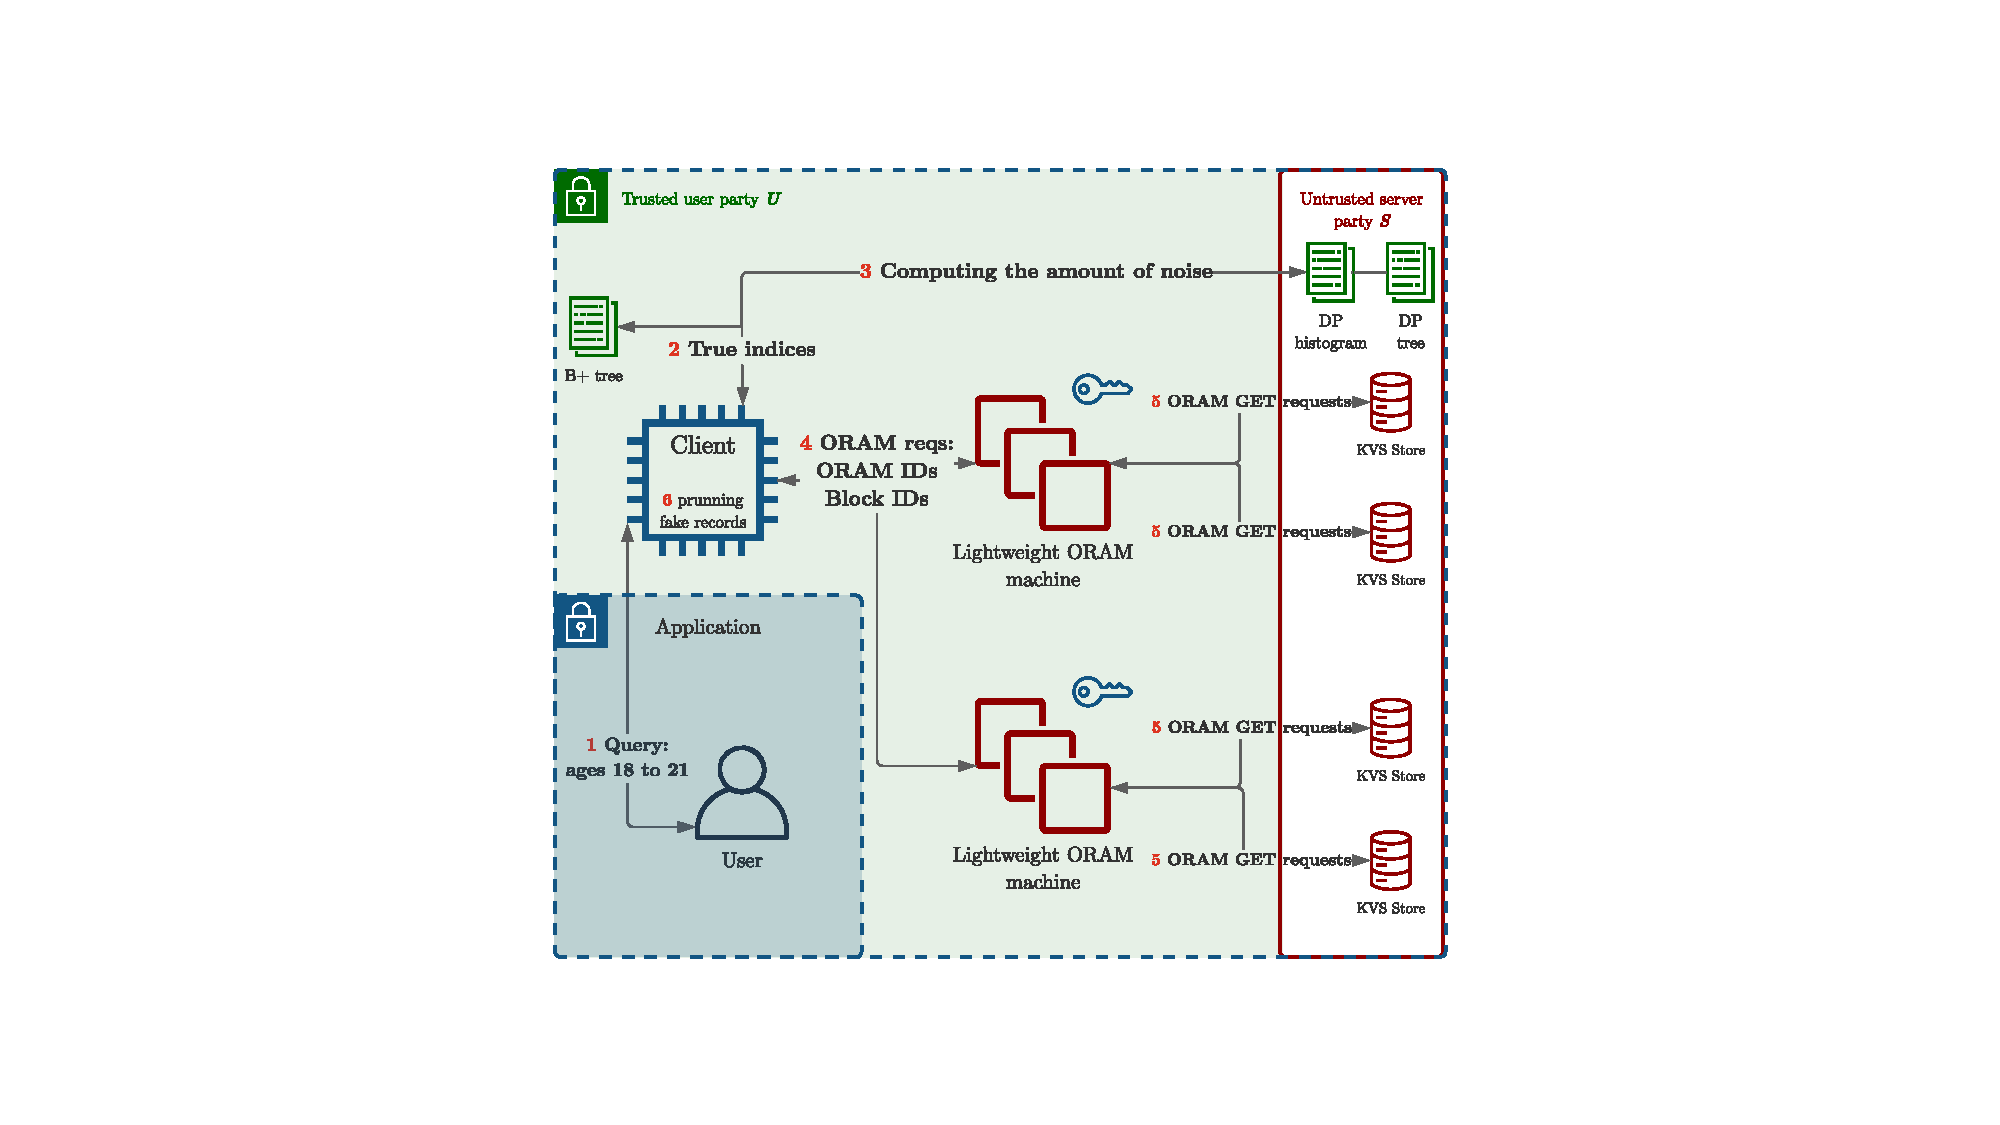
\includegraphics[width=\linewidth]{three-layers}
	\caption[Lightweight \acrshort{oram} machines diagram]{
		Lightweight \acrshort{oram} machines diagram.
		A \emph{user} sends a query to \user{} modeled as the \emph{client} machine, which uses local \emph{data index} and \emph{\acrshort{dp} structures} to prepare a set of \acrshort{oram} requests, which are sent to respective \emph{\acrshort{oram} machines}.
		These machines execute the \acrshort{oram} protocol against the \emph{untrusted storage} of \server{}.
	}%
	\label{figure:three-tier}
\end{figure}


			To address the problem, we split the user party \user{} into multiple lightweight machines that are connected locally to each other and reside in a single trust domain (e.g., same data center).
			Specifically, we maintain a \emph{client machine} that receives user requests and prepares \acrshort{oram} \texttt{read} requests, and up to \oramsNumber{} lightweight \emph{\acrshort{oram} machines}, whose only job is to run the \acrshort{oram} protocols in parallel.
			See \cref{figure:three-tier} for the schematic representation of the architecture.
			We emphasize that \user{} is still a single party, therefore, the security and correctness guarantees remain valid.

			The benefit of this approach is that each of the lightweight machines has its own hardware stack.
			Communication overhead among \user{} machines is negligible compared to the one between \user{} and \server{}.
			The approach is also flexible: it is possible to use up to \oramsNumber{} \acrshort{oram} machines and the machines do not have to be identical.
			Our experiments show that when the same number of \acrshort{cpu} cores and amount of memory are consumed the efficiency gain is up to \textbf{5 times}.

	\section{Experimental Evaluation}\label{section:range-persistent:experiments}

	We have implemented our solution as a modular client-server application in C++.
	We open-sourced all components of the software set: PathORAM\footnote{\url{https://github.com/epsolute/path-oram}} and B+ tree\footnote{\url{https://github.com/epsolute/b-plus-tree}} implementations and the main query executor\footnote{\url{https://github.com/epsolute/epsolute}}.
	We provide PathORAM and B+ tree components as C++ libraries to be used in other projects; the code is documented, benchmarked and tested (228 tests covering \SI{100}{\percent} of the code).
	We have also published our datasets and query sets.\footnote{\url{http://csr.bu.edu/dp-oram/}}

	For cryptographic primitives, we used OpenSSL library (version 1.1.1i).
	For symmetric encryption in \acrshort{oram} we have used \acrshort{aes} in \acrshort{cbc} mode \cite{aes-nist,nist-modes} with a 256-bits key (i.e., $\eta_2 = 2^{-256}$), for the hash algorithm \algo{H} used to partition records among \acrshortpl{oram} we have used \acrshort{sha}-256 algorithm \cite{nist-hash}.
	Aggregate tree fanout \fanout{} is 16, proven to be optimal in \cite{hierarchical-methods-for-dp}.

	We designed our experiments to answer the following questions:
	\newlength{\questionLength}
	\settowidth{\questionLength}{Question-5}
	\begin{description}[
		font=\bfseries,
		leftmargin=\dimexpr\questionLength+1.0em\relax,
		labelindent=0pt,
		labelwidth=\questionLength%
	]
		\item[Question-1\label{item:question-practicality}] How practical is our system compared to the most efficient and most private real-world solutions?
		\item[Question-2\label{item:question-storage}] How practical is the storage overhead?
		\item[Question-3\label{item:question-parameters}] How different inputs and parameters of the system affect its performance?
		\item[Question-4\label{item:question-scalability}] How well does the system scale?
		\item[Question-5\label{item:question-optimizations}] What improvements do our optimizations provide?
		\item[Question-6\label{item:question-attributes}] What is the impact of supporting multiple attributes?
	\end{description}

	For \ref{item:question-practicality} we have run the default setting using conventional \acrshort{rdbms} (MySQL and PostgreSQL), Linear Scan approach and Shrinkwrap \cite{shrinkwrap}. % chktex 2
	To target \ref{item:question-storage}, we measured the exact storage used by the client and the server for different data, record and domain sizes. % chktex 2
	To answer \ref{item:question-parameters}, we ran a default setting and then varied all parameters and inputs, one at a time. % chktex 2
	For \ref{item:question-scalability} we gradually added \acrshortpl{cpu}, \acrshort{oram} servers and \acrshort{kvs} instances and observed the rate of improvement in performance. % chktex 2
	To target \ref{item:question-optimizations} we have run the default setting with our optimizations toggled. % chktex 2
	Lastly, for \ref{item:question-attributes} we have used two datasets to construct two indices and then queried each of the attributes. % chktex 2

	\subsection{Data sets}\label{section:range-persistent:experiments:data-sets}

		We used two real and one synthetic datasets --- California public pay pension database 2019 \cite{ca-employees-dataset} (referred to as ``CA employees''), Public Use Microdata Sample from US Census 2018 \cite{pums-dataset} (referred to as ``PUMS'') and synthetic uniform dataset.
		We have used salary / wages columns of the real datasets, and the numbers in the uniform set also represent salaries.
		The \texttt{NULL} and empty values were dropped.

		We created three versions of each dataset --- $10^5$, $10^6$ and $10^7$ records each.
		For uniform dataset, we simply generated the target number of entries.
		For PUMS dataset, we picked the states whose number of records most closely matches the target sizes (Louisiana for $10^5$, California for $10^6$ and the entire US for $10^7$).
		Uniform dataset was also generated for different domain sizes --- number of distinct values for the record.
		For CA employees dataset, the set contains \num{260 277} records, so we contracted it and expanded in the following way.
		For contraction we uniformly randomly sampled $10^5$ records.
		For expansion, we computed the histogram of the original dataset and sampled values uniformly within the bins.

		Each of the datasets has a number of corresponding query sets.
		Each query set has a selectivity or range size, and is sampled either uniformly or following the dataset distribution (using its \acrshort{cdf}).

	\subsection{Default setting}\label{section:range-persistent:experiments:default-setting}

		The default setting uses the \protocolGamma{} from \cref{section:range-persistent:prallel-dp-oram} and lightweight \acrshort{oram} machines from \cref{section:range-persistent:dp-improvements:three-tier,figure:three-tier}.
		We choose the \protocolGamma{} because it outperforms \protocolNoGamma{} in all experiments (see \textbf{\ref{item:question-scalability}} in \cref{section:range-persistent:experiments:results}).
		In the setting, there are 64 Redis services (8 services per one Redis server \acrshort{vm}), 8 \acrshort{oram} machines communicating with 8 Redis services each, and the client, which communicates with these 8 \acrshort{oram} machines.
		We have empirically found this configuration optimal for the compute nodes and network that we used in the experiments.
		\acrshort{oram} and Redis servers run on \acrshort{gcp} \texttt{n1-standard-16} \acrshortpl{vm} (Ubuntu 18.04), in regions \texttt{us-east4} and \texttt{us-east1} respectively.
		Client machine runs \texttt{n1-highmem-16} \acrshort{vm} in the same region as \acrshort{oram} machines.
		The ping time between the regions (i.e.\ between trusted and untrusted zones) is \SI{12}{\milli\second} and the effective bandwidth is \SI{150}{\mega\byte\per\second}.
		Ping within a region is negligible.

		Default \acrshort{dp} parameters are $\epsilon = \ln(2) \approx \num{0.693}$ and $\beta = 2^{-20}$, which are consistent with the other \acrshort{dp} applications in the literature \cite{choosing-epsilon}.
		Buckets number is set as the largest power of $\fanout = 16$ that is no greater than the domain of the dataset \domainSize{}.

		Default dataset is a uniform dataset of $10^6$ records with domain size $10^4$, and uniformly sampled queries with selectivity \SI{0.5}{\percent}.
		Default record size is \SI{4}{\kibi\byte}.

	\subsection{Experiment stages}

		Each experiment includes running 100 queries such that the overhead is measured from loading query endpoints into memory to receiving the exact and whole query response from all \acrshort{oram} machines.
		The output of an experiment is, among other things, the overhead (in milliseconds), the number of real and noisy records fetched and communication volume averaged per query.

	\subsection{\texorpdfstring{\acrshort{rdbms}}{RDBMS}, Linear Scan and Shrinkwrap}

		On top of varying the parameters, we have run similar workloads using alternative mechanisms --- extremes representing highest performance or highest privacy.
		Unless stated otherwise, the client and the server are in the trusted and untrusted regions respectively, with the network configuration as in \cref{section:range-persistent:experiments:default-setting}.

		\subsubsection*{Relational databases}

			Conventional \acrshort{rdbms} represents the most efficient and least private and secure solution in our set.
			While MySQL and PostgreSQL offer some encryption options and no differential privacy, for our experiments we turned off security features for maximal performance.
			We have run queries against MySQL and PostgreSQL varying data and record sizes.
			We used \texttt{n1-standard-32} \acrshort{gcp} \acrshortpl{vm} in \texttt{us-east1} region, running MySQL version 14.14 and PostgreSQL version 10.14.

		\subsubsection*{Linear Scan}

			Linear scan is a primitive mechanism that keeps all records encrypted on the server then downloads, decrypts and scans the entire database to answer every query.
			This method is trivially correct, private and secure, albeit not very efficient.
			There are \acrshort{rdbms} solutions, which, when configured for maximum privacy, exhibit linear scan behavior (e.g., MS-SQL Always Encrypted with Randomized Encryption\footnote{\url{https://docs.microsoft.com/sql/relational-databases/security/encryption/always-encrypted-database-engine}} and Oracle Column Transparent Data Encryption\footnote{\url{https://docs.oracle.com/database/121/ASOAG/introduction-to-transparent-data-encryption.htm}}).
			For a fair comparison we make the linear scan even more efficient by allowing it to download data via parallel threads matching the number of threads and bytes per request to that of our solution.
			Although linear scan is wasteful in the amount of data it downloads and processes, compared to our solution it has a benefit of not executing an \acrshort{oram} protocol with its logarithmic overhead and network communication in both directions.

		\subsubsection*{Shrinkwrap}

			Shrinkwrap \cite{shrinkwrap} is a construction that answers federated \acrshort{sql} queries hiding both access pattern and communication volume.
			Using the \acrshort{emp} \cite{emp-toolkit} and the code Shrinkwrap authors shared with us, we implemented a prototype that only answers range queries.
			This part of Shrinkwrap amounts to making a scan over the input marking the records satisfying the range, sorting the input, and then revealing the result set plus \acrshort{dp} noise to the client.
			For the latter part we have adapted Shrinkwrap's Truncated Laplace Mechanism \cite[Definition 4]{shrinkwrap} to hierarchical method \cite{hierarchical-methods-for-dp} in order to be able to answer an unbounded number of all possible range queries.
			We have emulated the outsourced database setting by using two \texttt{n1-standard-32} servers in different regions (\SI{12}{\milli\second} ping and \SI{150}{\mega\byte\per\second} bandwidth) executing the algorithm in a circuit model (the faster option per Shrinkwrap experiments) and then revealing the result to the trusted client.
			We note that although the complexity of a Shrinkwrap query is $\bigO{n \log n}$ due to the sorting step, its functionality is richer as it supports more relational operators, like \texttt{JOIN}, \texttt{GROUP BY} and aggregation.
			We also note that since MySQL, PostgreSQL and Shrinkwrap are not parallelized within the query, experiments using more \acrshortpl{cpu} do not yield higher performance.

	\subsection{Results and Observations}\label{section:range-persistent:experiments:results}

		After running the experiments, we have made the following observations.
		Note that we report results based on the default setting.
		\begin{itemize}[leftmargin=*]
			\item
				\epsolute{} is efficient compared to a strawman approach, \acrshort{rdbms} and Shrinkwrap: it is three orders of magnitude faster than Shrinkwrap, 18 times faster than the scan and only 4--8 times slower than a conventional database.
				In fact, for different queries, datasets, and record sizes, our system is much faster than the linear scan, as we show next.
			\item
				\epsolute{}'s client storage requirements are very practical: client size is just below \SI{30}{\mega\byte} while the size of the offloaded data is over 400 times larger.
			\item
				\epsolute{} scales predictably with the change in its parameters: data size affects performance logarithmically, record size --- linearly, and privacy budget $\epsilon$ --- exponentially.
			\item
				\epsolute{} is scalable: using \protocolGamma{} with the lightweight \acrshort{oram} machines, the increase in the number of threads translates into linear performance boost.
			\item
				The optimizations proposed in \cref{section:range-persistent:dp-improvements} provide up to an order of magnitude performance gain.
			\item
				\epsolute{} efficiently supports multiple indexed attributes.
				The overhead and the client storage increase slightly due to a lower privacy budget and extra local indices.
		\end{itemize}

		For the purposes of reproducibility we have put the log traces of all our experiments along with the instructions on how to run them on a publicly available page \href{https://epsolute.org}{epsolute.org}.
		Unless stated otherwise, the scale in the figures is linear and the $x$-axis is categorical.

		\subsubsection*{\textbf{\texorpdfstring{\ref{item:question-practicality}:}{} against \acrshort{rdbms}, Linear Scan and Shrinkwrap}}

			\begin{figure}[!ht]
	\centering
	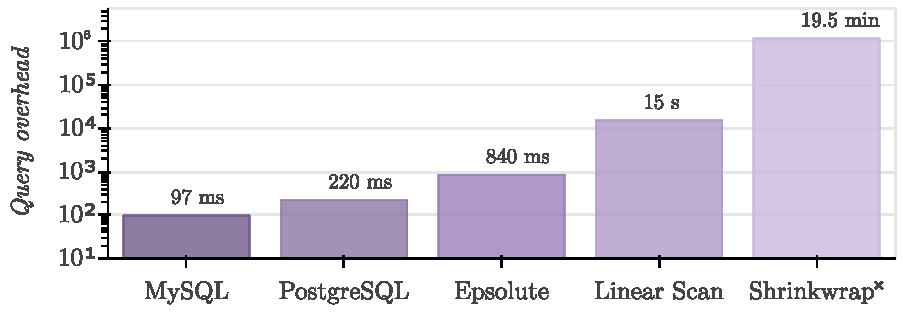
\includegraphics{mechanism}
	\caption[Different range-query mechanisms]{
		Different range-query mechanisms, logarithmic scale.
		Default setting: $10^6$ \SI{4}{\kibi\byte} uniformly-sampled records with the range $10^4$.
	}%
	\label{figure:mechanism}
\end{figure}


			The first experiment we have run using \epsolute{} is the default setting in which we observed the query overhead of \textbf{\SI[detect-all=true]{840}{\milli\second}}.
			To put this number in perspective, we compare \epsolute{} to conventional relational databases, the linear scan and Shrinkwrap.

			For the default setting, MySQL and PostgreSQL, configured for no privacy and maximum performance, complete in \SI{97}{\milli\second} and \SI{220}{\milli\second} respectively, which is just \textbf{8 to 4 times} faster than \epsolute{}, see \cref{figure:mechanism}.
			Conventional \acrshort{rdbms} uses efficient indices (B+ trees) to locate requested records and sends them over without noise and encryption, and it does so using less hardware resources.
			In our experiments \acrshort{rdbms} performance is linearly correlated with the result and record sizes.

			\begin{figure}[!ht]
	\centering
	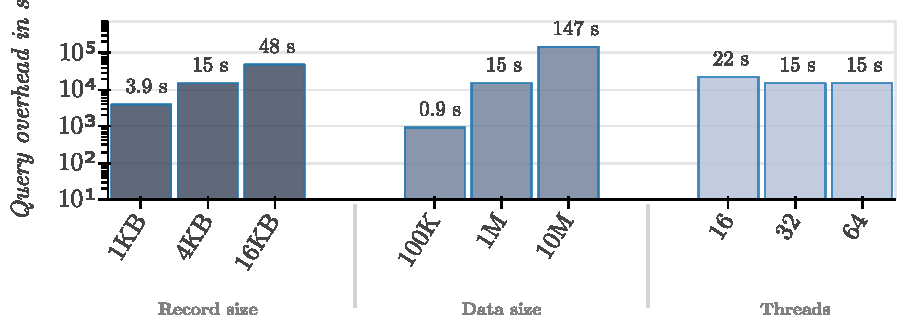
\includegraphics{linear-scan}
	\caption[Linear scan performance]{
		Linear scan performance, logarithmic scale.
		The experiments are run for the default setting of $10^6$ records of size \SI{4}{\kibi\byte} and 64 threads, with one of the three parameters varying.
	}%
	\label{figure:linear-scan}
\end{figure}


			Linear scan experiments demonstrate the practicality of \epsolute{} compared to a trivial ``download everything every time'' approach, see \cref{figure:linear-scan}.
			Linear scan's overhead is $\bigO{n}$ regardless of the queries, while \epsolute{}'s overhead is $\bigO{\log{n}}$ times the result size.
			According to our experiments, \epsolute{} eclipses the linear scan at \SI{4}{\kibi\byte}, 64 threads and only \emph{ten thousand records} (both mechanisms complete in about \SI{120}{\milli\second}).
			For a default setting (at a million records), the difference is \textbf{18 times}, see \cref{figure:linear-scan}.

			Because Shrinkwrap sorts the input obliviously in a circuit model, it then incurs $\bigO{n \log n}$ comparisons, each resulting in multiple circuit gates, which is much more expensive than the linear scan.
			Unlike linear scan, however, Shrinkwrap does not require much client memory as the client merely coordinates the query.
			While Shrinkwrap supports richer set of relational operators, for range queries alone \epsolute{} is \textbf{three orders of magnitude} faster.

		\subsubsection*{\textbf{\texorpdfstring{\ref{item:question-storage}:}{} storage}}

			% chktex-file 26
% chktex-file 8

\newcommand{\lightvbar}{\color{lightGrey}\vrule}
\newcommand{\lightcline}[1]{\arrayrulecolor{lightGrey}\cline{#1}\arrayrulecolor{black}}

\begin{table}[!ht]
	\renewcommand{\arraystretch}{1.2}
	\sisetup{detect-all = true}
	\begin{tabular*}{\linewidth}{ !{\extracolsep\fill} c | r !{\lightvbar{}} r | r !{\lightvbar{}} r | r !{\lightvbar{}} r} % chktex 44
		\toprule
			\diagbox{\dataSize}{\scriptsize{Record}}			& \multicolumn{2}{c !{\lightvbar{}}}{\SI{1}{\kibi\byte}}				& \multicolumn{2}{c !{\lightvbar{}}}{\SI{4}{\kibi\byte}}				& \multicolumn{2}{c}{\SI{16}{\kibi\byte}}												\\
		\midrule
			\multirow{2}{*}{$10^5$}								& \small\SI{400}{\kibi\byte}			& \small\SI{400}{\byte}			& \small\SI{400}{\kibi\byte}			& \small\SI{102}{\kibi\byte}	& \small\SI{400}{\kibi\byte}					& \small\SI{1.6}{\mega\byte}			\\ \lightcline{2-3} \lightcline{4-5} \lightcline{6-7}
																& \small\bfseries\SI{396}{\mega\byte}	& \small\SI{4.6}{\mega\byte}	& \small\bfseries\SI{1.5}{\giga\byte}	& \small\SI{14}{\mega\byte}		& \small\bfseries\SI{6.2}{\giga\byte}			& \small\SI{51}{\mega\byte}				\\

		\midrule
			\multirow{2}{*}{$10^6$}								& \small\SI{3.9}{\mega\byte}			& \small\SI{400}{\byte}			& \small\SI{3.9}{\mega\byte}			& \small\SI{102}{\kibi\byte}	& \small\SI{3.9}{\mega\byte}					& \small\SI{1.6}{\mega\byte}			\\ \lightcline{2-3} \lightcline{4-5} \lightcline{6-7}
																& \small\bfseries\SI{3.2}{\giga\byte}	& \small\SI{15}{\mega\byte}		& \small\bfseries\SI{12}{\giga\byte}	& \small\SI{25}{\mega\byte}		& \small\bfseries\SI{48}{\giga\byte}			& \small\SI{62}{\mega\byte}				\\

		\midrule
			\multirow{2}{*}{$10^7$}								& \small\SI{40}{\mega\byte}				& \small\SI{400}{\byte}			& \small\SI{40}{\mega\byte}				& \small\SI{102}{\kibi\byte}	& \small\itshape\SI{40}{\mega\byte}				& \small\itshape\SI{1.6}{\mega\byte}	\\ \lightcline{2-3} \lightcline{4-5} \lightcline{6-7}
																& \small\bfseries\SI{24}{\giga\byte}	& \small\SI{99}{\mega\byte}		& \small\bfseries\SI{96}{\giga\byte}	& \small\SI{109}{\mega\byte}	& \small\itshape\bfseries\SI{384}{\giga\byte}	& \small\itshape\SI{146}{\mega\byte}	\\

		\midrule
			\diagbox[dir=SW, width=6em]{\dataSize}{\domainSize}	& \multicolumn{2}{c !{\lightvbar{}}}{$100$}								& \multicolumn{2}{c !{\lightvbar{}}}{$10^4$}							& \multicolumn{2}{c}{$10^6$}															\\
		\toprule
	\end{tabular*}
	\sisetup{detect-none = true}
	\caption[Storage usage for varying data, record and domain sizes]{
		Storage usage for varying data, record and domain sizes.
		The values are as follows.
		Left top: index \indexI{} (B+ tree), right top: aggregate tree \serverDS{}, right bottom: \acrshort{oram} \user{} state and left bottom (bold): \acrshort{oram} \server{} state.
		\textit{Italic} indicates that the value is estimated.
	}%
	\label{table:storage}
\end{table}


			While \epsolute{} storage efficiency is near-optimal \efficiency{1}{0}, it is important to observe the absolute values.
			Index \indexI{} is implemented as a B+ tree with fanout 200 and occupancy \SI{70}{\percent}, and its size, therefore, is roughly $5.7 \dataSize$ bytes.
			Most of the \acrshort{oram} client storage is the PathORAM stash with its size chosen in a way to bound failure probability to about $\eta_1 = 2^{-32}$ (see \cite[Theorem 1]{path-oram}). % chktex 2
			In \cref{table:storage}, we present \epsolute{} storage usage for the parameters that affect it --- data, record and domain sizes.
			We measured the sizes of the index \indexI{}, \acrshort{dp} structure \serverDS{}, and \acrshort{oram} client and server states.
			Our observations are:
			\begin{enumerate*}[label={(\roman*)}]
				\item index size expectedly grows only with the data size,
				\item \serverDS{} is negligibly small in practice,
				\item small \indexI{} and \serverDS{} sizes imply the efficiency of supporting multiple indexed attributes,
				\item \server{} to \user{} storage size ratio varies from \textbf{85} in the smallest setting to more than \textbf{\num[detect-all=true]{2000}} in the largest, and
				\item one can trade client storage for \acrshort{oram} failure probability.
			\end{enumerate*}
			We conclude that the storage requirements of \epsolute{} are practical.

			% Stash size calculations are based on stash size 49, which, according to PathORAM paper, results in 14*0.6^{49} = 2^{-32} probability of failure

			% Total ORAM client size (in MB) is (( (2^h * 3 +3)*4 ) + (49 * (r * 1024) + 16))*64 / 1024^2
			% where h is ORAM_LOG_CAPACITY (11, 14, 17) and r is the record size in the number of kilobytes (1, 4, 16)

		\subsubsection*{\textbf{\texorpdfstring{\ref{item:question-parameters}:}{} varying parameters}}

			\begin{figure}[!ht]
	\centering
	\begin{minipage}{0.48\textwidth}
		\centering
		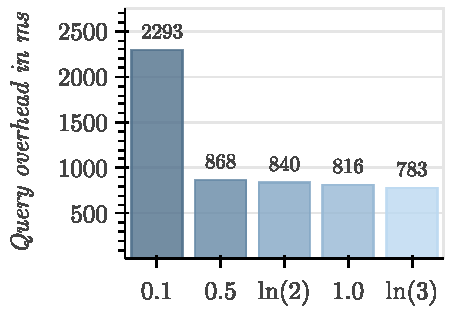
\includegraphics[width=\linewidth]{epsilon}
		\captionof{figure}{Privacy budget $\epsilon$}%
		\label{figure:epsilon}
	\end{minipage}
	~ % chktex 39
	\begin{minipage}{0.48\textwidth}
		\centering
		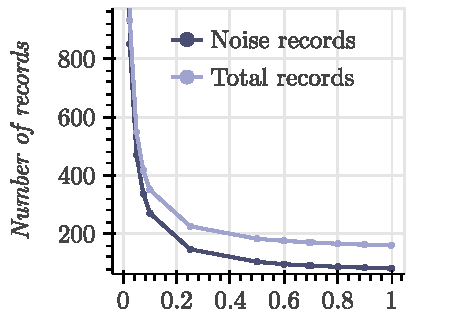
\includegraphics[width=\linewidth]{epsilon-effect}
		\captionof{figure}{Effect of $\epsilon$}%
		\label{figure:epsilon-effect}
	\end{minipage}
\end{figure}


			To measure and understand the impact of configuration parameters on the performance of our solution we have varied $\epsilon$, record size, data size \dataSize{}, domain size \domainSize{}, selectivities, as well as data and query distributions.
			The relation that is persistent throughout the experiments is that for given data and record sizes, the performance (the time to completely execute a query) is strictly proportional to the total number of records, fake and real, that are being accessed per query.
			Each record access goes through the \acrshort{oram} protocol, which, in turn, downloads, re-encrypts and uploads $\bigO{\log{\dataSize}}$ blocks.
			These accesses contribute the most to the overhead and all other stages (e.g., traversing index or aggregate tree) are negligible.

			\paragraph*{Privacy budget \texorpdfstring{$\epsilon$}{epsilon} and its effect}

				We have run the default setting for $\epsilon = \{ 0.1, \allowbreak 0.5, \allowbreak \ln{2}, \allowbreak 1.0, \allowbreak \ln{3} \}$.
				$\epsilon$ strictly contributes to the amount of noise, which grows exponentially as $\epsilon$ decreases, see \cref{figure:epsilon}, observe sharp drop.
				As visualized on \cref{figure:epsilon-effect}, at high $\epsilon$ values the noise contributes a fraction of total overhead, while at low values the noise dominates the overhead entirely.

			\begin{figure}[!ht]
	\centering
	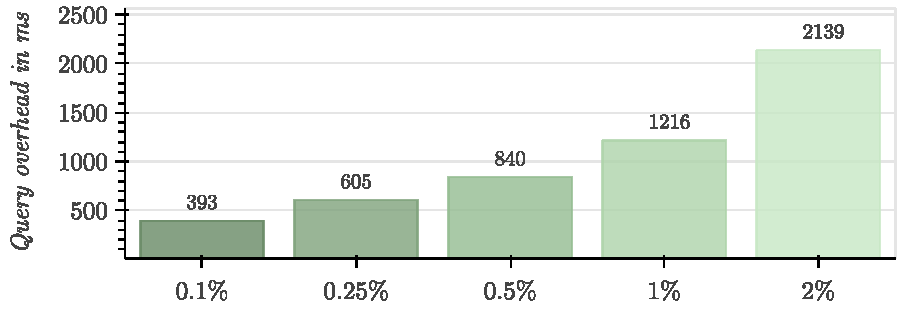
\includegraphics[width=\linewidth]{selectivity}
	\caption{Selectivity}%
	\label{figure:selectivity}
\end{figure}


			\paragraph*{Selectivity}

				We have ranged the selectivity from \SI{0.1}{\percent} to \SI{2}{\percent} of the total number of records, see \cref{figure:selectivity}.
				Overhead expectedly grows with the result size.
				For smaller queries, and thus for lower overhead, the relation is positive, but not strictly proportional.
				This phenomena, observed for the experiments with low resulting per-query time, is explained by the variance among parallel threads.
				During each query the work is parallelized over \oramsNumber{} \acrshortpl{oram} and the query is completed when the \emph{last} thread finishes.
				The problem, in distributed systems known as ``the curse of the last reducer'' \cite{curse-of-last-reducer}, is when one thread takes disproportionally long to finish.
				In our case, we run 64 threads in default setting, and the delay is usually caused by a variety of factors --- blocking \acrshort{io}, network delay or something else running on a shared virtual \acrshort{cpu}.
				This effect is noticeable when a single thread does relatively little work and small disruptions actually matter; the effect is negligible for large queries.

			\begin{figure}[!ht]
	\centering
	\begin{minipage}{0.31\columnwidth}
		\centering
		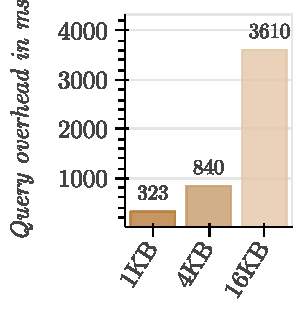
\includegraphics[width=\linewidth]{record-size}
		\captionof{figure}{Record size}%
		\label{figure:record-size}
	\end{minipage}
	~ % chktex 39
	\begin{minipage}{0.31\columnwidth}
		\centering
		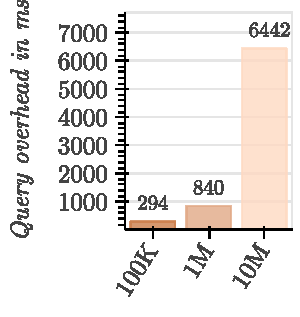
\includegraphics[width=\linewidth]{data-size}
		\captionof{figure}{Data size}%
		\label{figure:data-size}
	\end{minipage}
	~ % chktex 39
	\begin{minipage}{0.31\columnwidth}
		\centering
		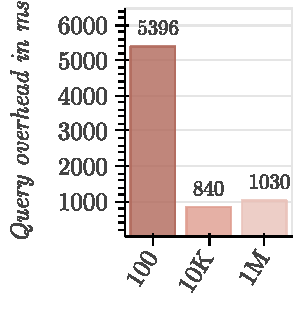
\includegraphics[width=\linewidth]{domain-size}
		\captionof{figure}{Domain size}%
		\label{figure:domain-size}
	\end{minipage}
\end{figure}


			\paragraph*{Record, data and domain sizes}

				We have tried \SI{1}{\kibi\byte}, \SI{4}{\kibi\byte} and \SI{16}{\kibi\byte} records, see \cref{figure:record-size}.
				Trivially, the elapsed time is directly proportional to the record size.

				We set \dataSize{} to $10^5$, $10^6$ and $10^7$, see \cref{figure:data-size}.
				The observed correlation of overhead against the data size is positive but non-linear, 10 times increment in \dataSize{} results in less than 10 times increase in time.
				This is explained by the \acrshort{oram} overhead --- when \dataSize{} changes, the \acrshort{oram} storage gets bigger and its overhead is logarithmic.

				For synthetic datasets we have set \domainSize{} to $100$, $10^4$ and $10^6$, see \cref{figure:domain-size}.
				The results for domain size correlation are more interesting: low and high values deliver worse performance than the middle value.
				Small domain for a large data set means that a query often results in a high number of real records, which implies significant latency regardless of noise parameters.
				A sparse dataset, on the other hand, means that for a given selectivity wider domain is covered per query, resulting in more nodes in the aggregate tree contributing to the total noise value.

			\begin{figure}[!ht]
	\centering
	\begin{minipage}{0.48\columnwidth}
		\centering
		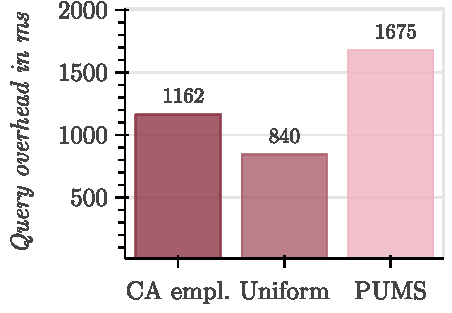
\includegraphics{data-distribution}
		\captionof{figure}{Data distribution}%
		\label{figure:data-distribution}
	\end{minipage}
	~ % chktex 39
	\begin{minipage}{0.48\columnwidth}
		\centering
		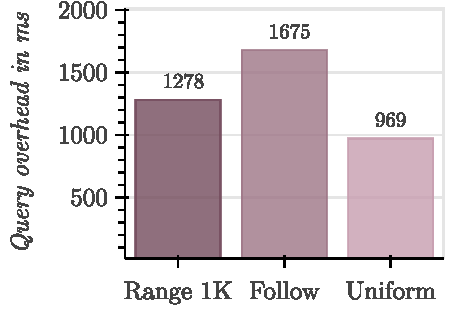
\includegraphics{query-distribution}
		\captionof{figure}{Query distribution}%
		\label{figure:query-distribution}
	\end{minipage}
\end{figure}


			\paragraph*{Data and query distributions}

				Our solution performs best on the uniform data and uniform ranges, see \cref{figure:data-distribution,figure:query-distribution}.
				Once a skew of any kind is introduced, there appear sparse and dense regions that contribute more overhead than uniform regions.
				Sparse regions span over wider range for a given selectivity, which results in more noise.
				Dense regions are likely to include more records for a given range size, which again results in more fetched records.
				Both real datasets are heavily skewed towards smaller values as few people have ultra-high salaries.

		\subsubsection*{\textbf{\texorpdfstring{\ref{item:question-scalability}:}{} scalability}}

			\begin{figure}[th]
	\centering
	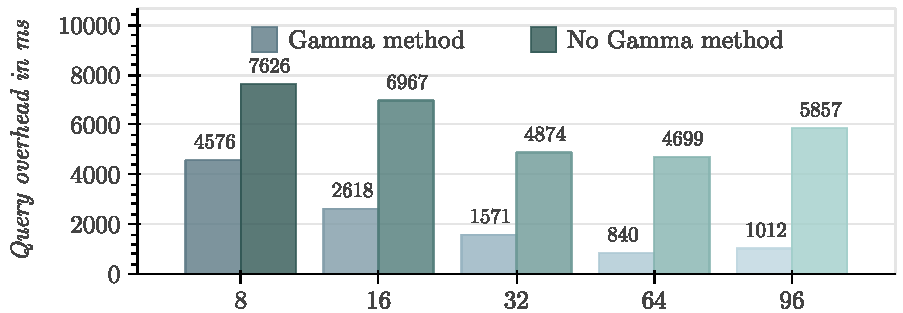
\includegraphics[width=\textwidth]{scalability}
	\caption[Scalability measurements for different methods of noise generation]{
		Scalability measurements for shared \serverDS{} structure \protocolGamma{} and separate \serverDS{} structures \protocolNoGamma{}
	}%
	\label{figure:scalability}
\end{figure}


			Horizontal scaling is a necessity for a practical system, this is the motivation for the parallelization in the first place.
			Ideally, performance should improve proportionally to the parallelization factor, number of \acrshortpl{oram} in our case, \oramsNumber{}.

			For scalability experiments we run the default setting for both \protocolNoGamma{} and \protocolGamma{} (\emph{no-$\gamma$-method} and \emph{$\gamma$-method} respectively) varying the number of \acrshortpl{oram} \oramsNumber{}, from 8 to 96 (maximum virtual \acrshortpl{cpu} on a \acrshort{gcp} \acrshort{vm}).
			The results are visualized on \cref{figure:scalability}.
			We report two positive observations:
			\begin{enumerate*}[label={(\roman*)}]
				\item the $\gamma$-method provides substantially better performance and storage efficiency, and
				\item when using this method the system scales linearly with the number of \acrshortpl{oram}.
			\end{enumerate*}
			($\oramsNumber = 96$ is a special case because some \acrshortpl{oram} had to share a single \acrshort{kvs}.)

		\subsubsection*{\textbf{\texorpdfstring{\ref{item:question-optimizations}:}{} optimizations benefits}}

			\begin{table}[!ht]
	\begin{tabular*}{\linewidth}{ !{\extracolsep\fill} l c c >{\bfseries}c } % chktex 26
		\toprule
			Improvement (section)													& Enabled					& Disabled					& Boost			\\
		\midrule
			\acrshort{oram} batching (\ref{section:dp-improvements:oram-batching})				& \SI{840}{\milli\second}	& \SI{6978}{\milli\second}	& 8.3x			\\
			Lightweight \acrshort{oram} machines (\ref{section:dp-improvements:three-tier})	& \SI{840}{\milli\second}	& \SI{4484}{\milli\second}	& 5.3x			\\
			Both improvements														& \SI{840}{\milli\second}	& \SI{8417}{\milli\second}	& \emph{10.0x}	\\
		\bottomrule
	\end{tabular*}
	\caption{Improvements over parallel \epsolute{}}%
	\label{table:optimizations}
\end{table}


			\cref{table:optimizations} demonstrates the boosts our improvements provide; when combined, the speedup is up to an order of magnitude.

			\acrshort{oram} request batching (\cref{section:range-persistent:dp-improvements:oram-batching}) makes the biggest difference.
			We have run the default setting with and without the batching.
			The overhead is substantially smaller because far fewer \acrshort{io} requests are being made, which implies benefits across the full stack: download, re-encryption and upload.

			Using lightweight \acrshort{oram} machines (\cref{section:range-persistent:dp-improvements:three-tier}) makes a difference when scaling.
			In the default setting, 64 parallel threads quickly saturate the memory access and network channel, while spreading computation among nodes removes the bottleneck.

		\subsubsection*{\textbf{\texorpdfstring{\ref{item:question-attributes}:}{} multiple attributes}}

			\begin{figure}[!ht]
	\centering
	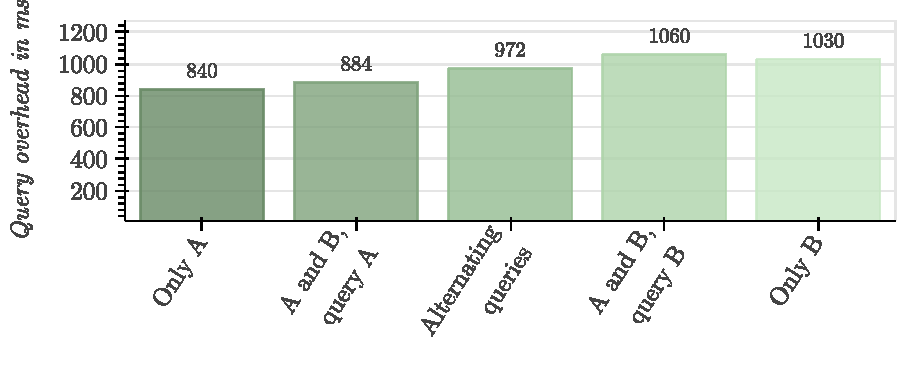
\includegraphics[width=\columnwidth]{multiple-attributes}
	\caption[Query overhead when using multiple attributes]{
		Query overhead when using multiple attributes.
		\emph{Only A} and \emph{Only B} index one attribute.
		\emph{A and B} indexes both attributes and then queries one of them.
		\emph{Alternating} indexes both attributes and runs half of the queries against \emph{A} and another half against \emph{B}.
	}%
	\label{figure:attributes}
\end{figure}


			\epsolute{} supports multiple indexed attributes.
			In \cref{section:range-persistent:dp-oram:multiple-attributes} we described that the performance implications amount to having an index \indexI{} and a \acrshort{dp} structure \serverDS{} per attribute and sharing the privacy budget $\epsilon$ among all attributes.
			As shown in \cref{table:storage}, \indexI{} and \serverDS{} are the smallest components of the client storage.
			To observe the query performance impact, we have used the default dataset with domains $10^4$ and $10^6$ as indexed attributes \emph{A} and \emph{B} respectively.
			We ran queries against only \emph{A}, only \emph{B} and against both attributes in alternating fashion.
			Each of the attributes used $\epsilon = \frac{\ln{2}}{2}$ to match the default privacy budget of $\ln(2)$.

			\cref{figure:attributes} demonstrates the query overhead of supporting multiple attributes.
			The principal observation is that the overhead increases only slightly due to a lower privacy budget.
			The client storage went up by just \SI{9}{\mega\byte}, and still constitutes only \SI{3.3}{\percent} of the server storage, which is not affected by the number of indexed attributes.

			% for 10K domain: total client storage went from 3.9+0.1+25 to 3.9+0.1+25+9, i.e. 31%
			% for 1M domain: total client storage went from 3.9+1.6+25 to 3.9+1.6+25+9, i.e. 29.5%


	\cleardoublepage%
	\chapter{\texorpdfstring{\acrshort{knn}}{kNN} queries in the snapshot model}\label{section:knn-snapshot}
\thispagestyle{myheadings}

	In this chapter I analyze secure \acrshort{knn} queries in the snapshot adversary model.
	I study the effect of protecting the records with a type of property-preserving encryption on quality of search and efficiency of certain attacks.
	Specifically, I examine theoretically and practically how accuracy of both \acrshort{knn} search and \acrshort{ml}-based inversion attack degrade with added security.

	\section{Introduction}

		Nearest-neighbor search is a type of optimization problem that, given a set of objects and a distance metric, requires finding the object closest to a given object according to the distance metric.
		A \acrfull{knn} search is a subtype of a general nearest-neighbor problem where $k$ closest objects are requested.
		Applications that use \acrshort{knn} search only need to define the objects and the metric.
		For example, a street map application would define the 2D coordinates of the buildings as objects and Euclidean distance as a metric, then the query could be ``give 5 restaurants closest to the current user position''.
		A document search application would define the keyword vector for a document as an object and an inner product distance as a metric, then the query could be ``give 3 documents most similar to the given text'' (similar applications may search images, videos and sounds).

		In this chapter we propose a method and an analysis of running secure \acrshort{knn} queries in outsourced database model.
		We model our application as a generic document similarity search, where the server stores the embeddings of the documents and returns $k$ closest records to the query embedding.
		We propose to apply a type of property-preserving encryption over the embeddings on the server while retaining its ability to do nearest-neighbor search.
		Finally, we simulate an attack against the records --- an \acrshort{ml}-based inversion attack that aims to recover the set of words of a document from its embeddings.
		Our goal is to observe and study the correlation of the security parameter with search accuracy and attack efficiency.

		To summarize, our contributions in this work are as follows:
		\begin{itemize}
			\item
				We adapt and implement a \acrfull{dcpe} scheme from \cite{dcpe} to encrypt text embeddings.
				We analyze the practical aspects of \acrshort{dcpe} scheme's security (e.g., the effects of floating point representation) and benchmark the construction.

			\item
				We conduct a set of experiments to study the effect of security parameter on search accuracy.
				We use a fine-tuned \acrshort{bert} model\footnote{Provided by Hamed Zamani} to produce embeddings for the \acrshort{trec} 2020 collection.
				Given \acrshort{trec} validation set (i.e., ``correct answers'') we run the search for varying security levels and report a number of ranking quality measures.

			\item
				We adapt a recent \acrshort{ml}-based inversion attack by \textcite{embedding-attacks} against embeddings to our setting.
				The attack works by training an \acrshort{lstm} model on pairs of sentences and their embeddings.
				We run this attack for varying security levels, and training on both plaintext and encrypted records.

			\item
				Finally, we analyze the correlation results for search accuracy and attack efficiency and conclude on practicality of our method.
		\end{itemize}

	\section{Related Work}

		Work in this area is naturally split into two groups --- mechanisms and constructions that offer certain security guarantees for nearest-neighbor queries, and attacks against those constructions.

		A work immediately related to ours is that of \textcite{quick-n}.
		QuickN offers an adaptation of nearest-neighbor search algorithm in conventional tree data structures (i.e., R-trees) to well-established \acrfull{ope} schemes.
		Unlike our solution that involves a novel property-preserving encryption scheme specifically designed for high-dimensional vectors, QuickN encrypts each vector dimension separately with \acrshort{ope}.
		\cite{quick-n} includes the experiments with attacks against their solution (attack of \textcite{leakage-abuse-grubs-2017}) and report high degree of protection against them.

		QuickN approach of applying \acrshort{ope} to an R-tree, however, has some disadvantages.
		First, an ideal stateless \acrshort{ope} has been shown inferior (\cite{ope-leakage}) to its counterpart, an \acrfull{ore} in which the comparison over ciphertexts is defined explicitly.\footnote{
			\cite{quick-n} uses mOPE \cite{ope-ideal-security-protocol} which is an interactive protocol and not a traditional lightweight stateless \acrshort{ope} like \cite{bclo-ope}.
			Since mOPE is an ideal (though stateful) \acrshort{ope}, \cite{quick-n} do not include \acrshort{ope} leakage in their security definition.
		}
		An \acrshort{ore}, in turn, can have a varying level of security, with the higher security level translating into lower comparison performance.
		In QuickN, an R-tree-based nearest-neighbor algorithm involves a very high number of comparisons, linear in data dimensionality.
		With the cost of comparison no longer negligible, the overhead of query over 2D or 3D is already high, saying nothing of 768-dimensional vectors that our work targets.
		Second, QuickN protocol is not single-round (i.e., it takes two roundtrips per query) and it returns a large number of false positive results even for a minimal $k$ (\num{4000} false positives for $10^6$ dataset and $k = 1$).

		\textcite{knn-aspe} offer a novel scheme, ASPE, that preserves a special type of scalar product.
		ASPE is then naturally integrated in existing \acrshort{knn} algorithms that rely on a scalar product.
		\cite{knn-aspe} is similar to ours in that we also apply a property-preserving encryption scheme to existing \acrshort{knn} algorithms.
		ASPE is different in that it preserves a scalar product while we preserve an L2 distance comparison, and ASPE has been broken in \cite{secure-nn-revisited-break-aspe} (although an attack is a chosen plaintext attack, i.e., one cannot decrypt a random ciphertext).

		Other works either target different aspects of query security, like integrity and soundness of results \cite{knn-integrity-soundness,svknn}, or involve mechanisms other than property-preserving encryption \cite{seceqp,practical-approx-knn,knn-sharing-keys,knn-mult-data-owners,knn-over-encrypted,knn-paillier,knn-blind,knn-homomorphism,knn-strong-location-privacy,knn-no-anonymizers,knn-efficient,knn-new-casper}.

	\section{\texorpdfstring{\acrlong{dcpe}}{Distance Comparison Preserving Encryption}}

		A promising approach in secure \acrshort{knn} evaluation is using a property-preserving encryption scheme to allow the existing search algorithms to work with minimal alterations.
		ASPE scheme by \textcite{knn-aspe} is a step in this direction, but a scheme has been shown insecure under a type of chosen plaintext attack in \cite{secure-nn-revisited-break-aspe}.
		Using a common \acrshort{ope} scheme over vector values has been explored in \cite{quick-n}, but this approach incurs high overhead linear in dimensionality.
		We, therefore, need a different method --- a scheme that operates over high-dimensional vectors and preserves a property that is required to answer the nearest-neighbor queries.

		A classical nearest-neighbor search \cite{knn-wong,knn-cunningham} simply orders the objects according to their distances from the target.
		It is important to note that knowing the exact distance is not required, merely the knowledge of \emph{distance comparison} suffices (i.e., $x$ is closer to $y$ than $z$ is).
		An encryption scheme that preserves the distance comparison would satisfy the \acrshort{knn} search correctness, but not necessarily security or even practicality.
		First, a fully deterministic \acrfull{dcpe} would reveal at least the frequency of data points (i.e., how many times a point appears in the dataset).
		Second, even in the plaintext world the use of approximate nearest-neighbor search \cite{scalable-nn,approximate-nn-fixed-d} may be preferred due to the curse of dimensionality \cite{nn-meaningful,nn-curse-of-d} (exact distance is less important in higher dimensions).

		\subsection{\texorpdfstring{\acrshort{dcpe}}{DCPE} construction}

			A candidate \emph{approximate} \acrshort{dcpe} scheme that we adapt to our solution has been recently proposed by \textcite{dcpe}.
			The scheme provides the following guarantee on its ciphertexts
			\begin{multline*}
				\forall x, y, z \in \mathbb{X} : \algo{Dist}{x, y} < \algo{Dist}{x, z} - \beta \\
				\implies \algo{Dist}{f(x), f(y)} < \algo{Dist}{f(x), f(z)}
			\end{multline*}
			where $\mathbb{X} \subseteq \mathbb{R}^d$ is the set of $d$-dimensional vectors of real numbers, \algo{Dist} is the inner product distance over elements in $\mathbb{X}$, and $\beta$ is the approximation term.
			Parameter $\beta$ partially defines the security of the encrypted set --- the larger $\beta$, the fewer distance comparisons are preserved, the less accurate the search and the reconstruction attacks would be.
			\textcite{dcpe} prove protection against membership inference attacks \cite{memebership-inference-attacks-knn} (whether an individual is in the database or not), and against approximate frequency-finding attacks (how many times the element appears in the set, see \cite{leakage-abuse-grubs-2017} for \acrshort{ore} frequency attacks).
			As for the choice of $\beta$, \textcite{dcpe} proves that $\beta \approx \sqrt{\max N}$ would hide about half of the input bits, for $\max N$ being the maximum vector length in the dataset.

			% chktex-file 1
% chktex-file 8

\newlength{\dcpeAlgInterLength}
\setlength{\dcpeAlgInterLength}{0.18ex}

\begin{algorithm*}[ht!]

	\begin{pchstack}

		\procedure[linenumbering]{\algo{KeyGen}{\secparam, \mathbb{S}}}{
			s \sample \mathbb{S}		\\
			\key \sample \bin^\secpar	\\
			\pcreturn (s, \key)
		}

		\hspace{\dcpeAlgInterLength}

		\procedure[linenumbering]{\algo{Enc}{ (s, \key), \vec{m} }}{
			n \sample \bin^\secpar														\\
			\mathsf{coins}_n || \mathsf{coins}_u \gets \algo{\acrshort{prf}}{\key, n}	\\
			\vec{n} \sample \algo{Normal}{0, I_d; \mathsf{coins}_n}						\\
			u \sample \algo{Uniform}{0, 1; \mathsf{coins}_u}							\\
			x \gets \frac{s \beta}{4} \cdot \sqrt[d]{u}									\\
			\vec{\delta} \gets \frac{\vec{n}}{\|\vec{n}\|} \cdot x						\\
			\vec{c} \gets s \cdot \vec{m} + \vec{\delta}								\\
			\pcreturn \vec{c}
		}

		\hspace{\dcpeAlgInterLength}

		\procedure[linenumbering]{\algo{Dec}{ (s, \key), (\vec{c}, n) }}{
			\mathsf{coins}_n || \mathsf{coins}_u \gets \algo{\acrshort{prf}}{\key, n}	\\
			\vec{n} \sample \algo{Normal}{0, I_d; \mathsf{coins}_n}						\\
			u \sample \algo{Uniform}{0, 1; \mathsf{coins}_u}							\\
			x \gets \frac{s \beta}{4} \cdot \sqrt[d]{u}									\\
			\vec{\delta} \gets \frac{\vec{n}}{\|\vec{n}\|} \cdot x						\\
			\vec{m} \gets \frac{\vec{c} - \vec{\delta}}{s}								\\
			\pcreturn \vec{m}
		}

	\end{pchstack}

	\caption[\acrshort{dcpe} scheme]{
		\acrlong{dcpe} scheme, adapted from \cite[Algorithm 2]{dcpe}.
	}%
	\label{algorithm:dcpe}
\end{algorithm*}


			\textcite{dcpe} offer an instantiation of the $\beta$-\acrshort{dcpe} scheme (though not an implementation) that we have adapted for our needs and show on \cref{algorithm:dcpe}.

			The \algo{KeyGen} procedure generates a key \key{} and an amplification factor $s$.

			The \algo{Enc} procedure ``encrypts'' an object by moving it in space in a way that it is hard to recover its original position and its distance-comparison respective to other encrypted points is preserved.
			The algorithm first constructs a hyperball of radius $\beta$, the approximation term, around the input point.
			The routine then samples a new point uniformly inside that hyperball.
			Finally, that new point is projected into the ciphertext point according to the amplification factor $s$.
			Note that for each encryption the scheme generates a nonce $n$ and uses it along with the key \key{} to generate the coins for the samplers.
			That is, the point in the $\beta$-hyperball is deterministically set from the nonce (unique per point) and the key (one for all points), and the final ciphertext is scaled the same way for all points.
			The \algo{Dec} procedure makes the same steps in reverse correctly setting the point in the hyperball using the nonce and the key.
			See \cref{figure:dcpe} for a visual example of \acrshort{dcpe} encryption.

			\begin{figure}[!ht]
	\centering
	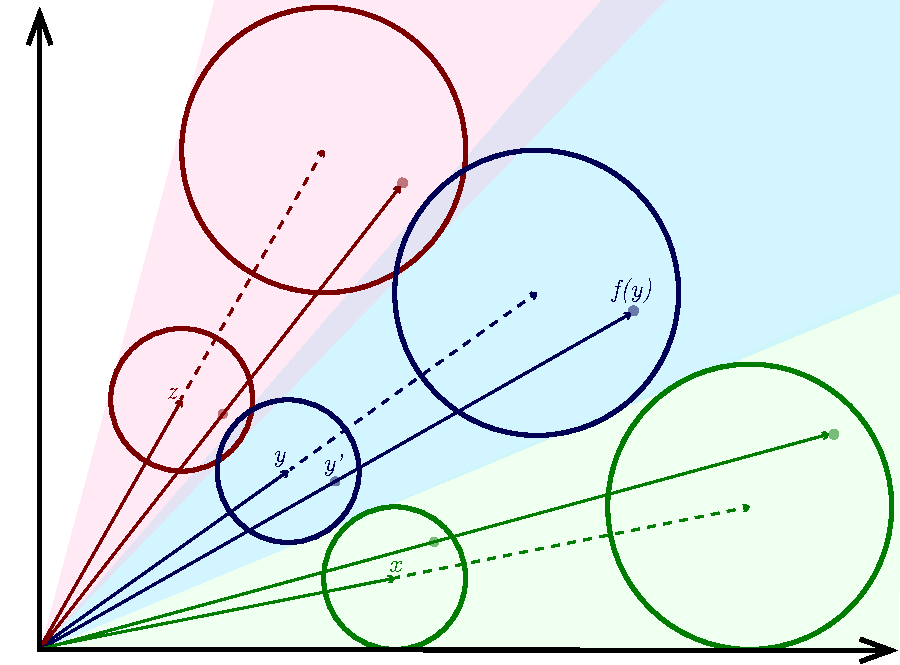
\includegraphics[width=1.0\textwidth]{dcpe}
	\caption[Schematic description of \acrshort{dcpe}]{
		Schematic description of encryption process of \acrshort{dcpe}, drawn to scale.
		In this diagram, there are two dimensions ($d = 2$), $\beta$ (the radius of a circle) is 2 units, and $s$ (the projection magnitude, the length from the origin to the larger circle over the length to the smaller one) is 2.
		The encrypted point is uniformly sampled inside a $\beta$-sphere, then projected $s$ times further from the origin.
		If two points are too close, their circles intersect, and their encryptions can be sampled in a way that breaks distance comparison.
		Intuitively, larger $\beta$ implies greater ciphertext space for a point and greater security.
	}\label{figure:dcpe}
\end{figure}


		\subsection{\texorpdfstring{\acrshort{dcpe}}{DCPE} security}

			The security of the scheme thus depends on
			\begin{enumerate*}[label={(\roman*)}]
				\item the maximum amount of amplification,
				\item the radius of the hyperball $\beta$, and
				\item the entropy of the samplers.
			\end{enumerate*}
			\textcite{dcpe} show that the amplification, $s$ parameter, affects one-wayness bounds \cite[Section 7.2]{dcpe}.
			Approximation term $\beta$ affects bit-security with $\beta \approx \sqrt{\max N}$ protecting about half of the bits.
			Finally, the key \key{} and nonce $n$ sizes, the security parameter \secparam{}, and the samplers used to generate normal multivariate and uniform samples affect the specific amount of entropy used to generate a point in the hyperball.

			As the construction operates on real numbers, an open question remains on how to avoid negative side-effects of floating point numbers bit representation.
			Unlike integers, floating point numbers are represented in memory in a way that their precision is different depending on their value, see the IEEE 754-2019 standard \cite{ieee-floating-point}. % chktex 8
			Simply put, the closer the value is to zero, the smaller the difference between two consecutive representable values is.
			For example, while the representable 32-bit IEEE 754 floating point numbers range from about $1.18 \cdot 10^{-38}$ to $3.4 \cdot 10^{38}$, there are only $2^{32} \approx 4 \cdot 10^9$, 4 billion representable numbers.
			This, along with the rounding errors, puts some limits on how large $s$ and $\beta$ can be.

		\subsection{\texorpdfstring{\acrshort{dcpe}}{DCPE} implementation and benchmarks}

			We offer the first implementation of \cite{dcpe} $\beta$-\acrshort{dcpe} for 32- and 64-bit IEEE 754 numbers in C++.\footnote{
				\url{https://github.com/private-knn/dcpe}
			}
			The code is documented, tested and benchmarked, see \cref{table:dcpe-benchmarks}.
			Observe that the difference in performance between encryption and decryption is predictably minimal, and the overhead of encryption grows slower than linearly with dimensionality.
.
			{
	\def\arraystretch{1.0}
	\begin{table}[!ht]
		\begin{tabular*}{\linewidth}{ !{\extracolsep\fill} l l c l } % chktex 26
			\toprule
				Operation						& Input size								& Dimensions $d$	& Wall-clock time			\\
			\midrule
				\algo{KeyGen}					& N/A										& N/A				& \SI{1.81}{\milli\second}	\\
			\midrule
				\multirow{6}{*}{\algo{Enc}}		& \multirow{3}{*}{32-bit (\texttt{float})}	& 1					& \SI{4.12}{\milli\second}	\\
												& 											& 100				& \SI{12.2}{\milli\second}	\\
												& 											& 768				& \SI{62.0}{\milli\second}	\\ \cline{2-4}
												& \multirow{3}{*}{64-bit (\texttt{double})}	& 1					& \SI{3.96}{\milli\second}	\\
												& 											& 100				& \SI{11.4}{\milli\second}	\\
												& 											& 768				& \SI{59.3}{\milli\second}	\\
			\midrule
				\multirow{6}{*}{\algo{Dec}}		& \multirow{3}{*}{32-bit (\texttt{float})}	& 1					& \SI{3.94}{\milli\second}	\\
												& 											& 100				& \SI{11.6}{\milli\second}	\\
												& 											& 768				& \SI{62.1}{\milli\second}	\\ \cline{2-4}
												& \multirow{3}{*}{64-bit (\texttt{double})}	& 1					& \SI{3.96}{\milli\second}	\\
												& 											& 100				& \SI{11.3}{\milli\second}	\\
												& 											& 768				& \SI{59.6}{\milli\second}	\\
			\bottomrule
		\end{tabular*}
		\caption{\acrshort{dcpe} implementation benchmarks}%
		\label{table:dcpe-benchmarks}
	\end{table}
}

% cSpell:disable

% ref: e9fd950
% ❯ make clean run-benchmarks                                                                             04:24:23 PM
% rm -rf ../docs
% rm -rf bin/*
% rm -rf obj/* *~ *.dSYM *.gcov *.gcda *.gcno *.bin coverage-html junit-*.xml cobertura.xml
% clang++ -c -o obj/utility.o src/utility.cpp -I/opt/homebrew/opt/openssl@3/include -I/opt/homebrew/Cellar/boost/1.76.0/include -I/opt/homebrew/opt/llvm/include --std=c++2a -Wall -Wno-unknown-pragmas -fPIC -I include
% clang++ -c -o obj/scheme.o src/scheme.cpp -I/opt/homebrew/opt/openssl@3/include -I/opt/homebrew/Cellar/boost/1.76.0/include -I/opt/homebrew/opt/llvm/include --std=c++2a -Wall -Wno-unknown-pragmas -fPIC -I include
% clang++ -o bin/benchmark-utility obj/utility.o obj/scheme.o benchmark/benchmark-utility.cpp -I/opt/homebrew/opt/openssl@3/include -I/opt/homebrew/Cellar/boost/1.76.0/include -I/opt/homebrew/opt/llvm/include --std=c++2a -Wall -Wno-unknown-pragmas -fPIC -I include -l boost_system  -l gtest -l pthread -l benchmark  -L/opt/homebrew/opt/openssl@3/lib -L/opt/homebrew/Cellar/boost/1.76.0/lib -L/opt/homebrew/opt/llvm/lib -L lib
% clang++ -o bin/benchmark-scheme obj/utility.o obj/scheme.o benchmark/benchmark-scheme.cpp -I/opt/homebrew/opt/openssl@3/include -I/opt/homebrew/Cellar/boost/1.76.0/include -I/opt/homebrew/opt/llvm/include --std=c++2a -Wall -Wno-unknown-pragmas -fPIC -I include -l boost_system  -l gtest -l pthread -l benchmark  -L/opt/homebrew/opt/openssl@3/lib -L/opt/homebrew/Cellar/boost/1.76.0/lib -L/opt/homebrew/opt/llvm/lib -L lib
% bin/benchmark-utility&& bin/benchmark-scheme&& echo Benchmarks completed!
% Unable to determine clock rate from sysctl: hw.cpufrequency: No such file or directory
% 2022-03-23T16:25:25-04:00
% Running bin/benchmark-utility
% Run on (10 X 24.1209 MHz CPU s)
% CPU Caches:
%   L1 Data 64 KiB (x10)
%   L1 Instruction 128 KiB (x10)
%   L2 Unified 4096 KiB (x5)
% Load Average: 3.31, 2.42, 2.17
% ------------------------------------------------------------------------------------------------------
% Benchmark                                                            Time             CPU   Iterations
% ------------------------------------------------------------------------------------------------------
% UtilityBenchmark<float>/Random/iterations:1048576                0.031 us        0.030 us      1048576
% UtilityBenchmark<float>/Uniform_float/iterations:1048576          1.68 us         1.68 us      1048576
% UtilityBenchmark<double>/Uniform_double/iterations:1048576        1.72 us         1.72 us      1048576
% UtilityBenchmark<float>/Normal_float/1/iterations:32768           1.99 us         1.98 us        32768
% UtilityBenchmark<float>/Normal_float/2/iterations:32768           2.07 us         2.07 us        32768
% UtilityBenchmark<float>/Normal_float/3/iterations:32768           2.14 us         2.14 us        32768
% UtilityBenchmark<float>/Normal_float/10/iterations:32768          2.61 us         2.61 us        32768
% UtilityBenchmark<float>/Normal_float/100/iterations:32768         7.32 us         7.32 us        32768
% UtilityBenchmark<double>/Normal_double/1/iterations:32768         1.97 us         1.97 us        32768
% UtilityBenchmark<double>/Normal_double/2/iterations:32768         2.06 us         2.06 us        32768
% UtilityBenchmark<double>/Normal_double/3/iterations:32768         2.13 us         2.13 us        32768
% UtilityBenchmark<double>/Normal_double/10/iterations:32768        2.55 us         2.55 us        32768
% UtilityBenchmark<double>/Normal_double/100/iterations:32768       7.06 us         7.06 us        32768
% Unable to determine clock rate from sysctl: hw.cpufrequency: No such file or directory
% 2022-03-23T16:25:30-04:00
% Running bin/benchmark-scheme
% Run on (10 X 24.1206 MHz CPU s)
% CPU Caches:
%   L1 Data 64 KiB (x10)
%   L1 Instruction 128 KiB (x10)
%   L2 Unified 4096 KiB (x5)
% Load Average: 3.61, 2.49, 2.20
% ------------------------------------------------------------------------------------------------------
% Benchmark                                                            Time             CPU   Iterations
% ------------------------------------------------------------------------------------------------------
% SchemeBenchmark<float>/KeyGen_float/iterations:1048576            1.81 us         1.81 us      1048576
% SchemeBenchmark<double>/KeyGen_double/iterations:1048576          1.79 us         1.79 us      1048576
% SchemeBenchmark<float>/Encrypt_float/1/iterations:32768           4.12 us         4.12 us        32768
% SchemeBenchmark<float>/Encrypt_float/100/iterations:32768         12.2 us         12.2 us        32768
% SchemeBenchmark<float>/Encrypt_float/768/iterations:32768         62.0 us         62.0 us        32768
% SchemeBenchmark<double>/Encrypt_double/1/iterations:32768         3.96 us         3.96 us        32768
% SchemeBenchmark<double>/Encrypt_double/100/iterations:32768       11.4 us         11.4 us        32768
% SchemeBenchmark<double>/Encrypt_double/768/iterations:32768       59.3 us         59.3 us        32768
% SchemeBenchmark<float>/Decrypt_float/1/iterations:32768           3.94 us         3.94 us        32768
% SchemeBenchmark<float>/Decrypt_float/100/iterations:32768         11.6 us         11.6 us        32768
% SchemeBenchmark<float>/Decrypt_float/768/iterations:32768         62.1 us         62.1 us        32768
% SchemeBenchmark<double>/Decrypt_double/1/iterations:32768         3.96 us         3.96 us        32768
% SchemeBenchmark<double>/Decrypt_double/100/iterations:32768       11.3 us         11.3 us        32768
% SchemeBenchmark<double>/Decrypt_double/768/iterations:32768       59.6 us         59.6 us        32768
% Benchmarks completed!


	\section{\texorpdfstring{\acrshort{knn}}{kNN} search accuracy}\label{section:knn-snapshot:search}

		The first part of a practical and secure outsourced similarity search application is the search accuracy.
		In this set of experiments we embed the documents and apply $\beta$-\acrshort{dcpe} to the embeddings.
		We use existing efficient nearest-neighbor search algorithms and report on ranking quality metrics for different $\beta$.

		\subsection{Secure \texorpdfstring{\acrshort{knn}}{kNN} protocol}

			With the $\beta$-\acrshort{dcpe} as a component, we can model the protocols similar to \acrshort{ore} ones.
			In the setup protocol \protocolSetup{}, \user{} simply encrypts the entire input, one vector at a time, and sends the encrypted data over to \server{}.
			In the query protocol \protocolQuery{}, \user{} encrypts the query with \acrshort{dcpe}, sends the ciphertext to \server{}, while \server{} runs a standard \acrshort{knn} search against the ciphertext.
			$k$ encrypted vectors are then returned to \user{}, who decrypts them as the last step.
			These protocols are run for a single set of secrets and \acrshort{dcpe} parameters, including $\beta$.

			For the choice of the dataset, we use the established information retrieval \acrshort{trec} 2020 test collections.
			A \acrshort{trec} collection consists of a set of documents, a set of topics (questions) and a corresponding set of relevance judgments (correct answers).
			A benefit of using a \acrshort{trec} dataset is being able to evaluate relevant metrics over the produced results, for example, \acrshort{mrr} \cite{mrr} and \acrshort{ndcg} \cite{dcg}.
			We can then track how these metrics, along with the simpler edit distance and set difference over the result, degrade with higher security.

			As the embedding mechanism, we use a custom fine-tuned \acrshort{bert} model.\footnote{Provided by Hamed Zamani}
			\acrfull{bert} is a transformer-based \acrshort{ml} technique for \acrlong{nlp}.
			An original \acrshort{bert} model, published by \textcite{bert}, has been trained on a BookCorpus \cite{bookcorpus} (800 million words) and English Wikipedia (2.5 billion words) using 24 encoders with 16 bidirectional self-attention heads (for the larger of two versions, $\text{\acrshort{bert}}_\text{LARGE}$).
			\acrshort{bert}'s main novelty is its bidirectional nature --- it processes all words in relation to each other and not one-by-one.
			The technology is now prevalent \cite{bert-is-prevalent}, and Google uses \acrshort{bert} in almost every English query\footnote{
				\url{https://searchengineland.com/google-bert-used-on-almost-every-english-query-342193}
			}.
			It is common, however, to use the original \acrshort{bert} model as a base and do training on top.
			{\color{red}We use one of such fine-tuned \acrshort{bert} models for embedding.}

		\subsection{Experimental evaluation}

			The actual experiment is conducted as follows.
			First, we produce a set of embeddings for 8.8 million documents and 200 queries from \acrshort{trec} 2020 dataset.
			We observed that the maximum length of an embedding vector is about 11 units.
			Second, we encrypt the data and queries embeddings using \acrshort{dcpe} and ranging $\beta$ from 0 (meaning exact distance-comparison) to 50, with $\beta = \sqrt{11} \approx 3.3$ hiding about half of the bits of input embeddings.
			Third, we run the nearest neighbor search on these pairs of data and queries sets using \acrshort{faiss} \cite{faiss}, a \acrshort{gpu}-enabled library for efficient similarity search and clustering of dense vectors.
			Finally, we report a range of ranking quality metrics and generic \acrshort{knn} result metrics.

			\subsubsection{Ranking quality metrics}

				We report recall, \acrfull{mrr} \cite{mrr} and \acrfull{ndcg} \cite{dcg} metrics to assess the ranking quality with respect to \acrshort{trec} relevance judgments.

				\emph{Recall} is fraction of relevant documents that the query retrieved over all relevant documents.

				\acrfull{mrr} is the average of reciprocal ranks of a query response, which is a multiplicative inverse of the rank of the first correct answer.
				\acrshort{mrr} is defined as
				\[
					\mathsf{\acrshort{mrr}} = \frac{1}{| \mathbb{Q} |} \sum_{i = 1}^{| \mathbb{Q} |} \frac{1}{\mathsf{rank}_i} \; ,
				\]
				where $\mathbb{Q}$ is the sample of queries and $\mathsf{rank}_i$ is the rank position of the first relevant document for the $i_\text{th}$ query.

				\acrfull{ndcg} is another measure of ranking quality most used in web search engine algorithms.
				Its main goal is to produce a metric that would promote these two assumptions.
				First, documents' relevance implies its usefulness, and second, highly relevant documents are more useful if they have higher rank (appear earlier in result list).
				\acrshort{ndcg} is a normalized version of discounted cumulative gain, and is defined as the actual over ideal gain up to a position $p$
				\[
					\mathsf{\acrshort{ndcg}}_p = \frac{\mathsf{DCG}_p}{\mathsf{IDCG}_p} = \frac{ \sum_{i=1}^p \frac{ \mathsf{relevance}_i }{ \log_2 (i + 1) } }{ \sum_{i=1}^{ \algo{Rel}{p} } \frac{ \mathsf{relevance}_i }{ \log_2 (i + 1) } } \; ,
				\]
				where $\mathsf{relevance}_i$ is the graded relevance of the result at position $i$ and $\algo{Rel}{p}$ is the number of relevant documents in the corpus up to position $p$.
				Note that we use a classic definition from \cite{dcg}, and not the \cite{dcg-updated} definition that puts even greater emphasis on relevance.

				We measure all three metrics at certain cutoffs, meaning that if the number of returned documents is smaller than the cutoff, the missing documents are assumed to be irrelevant.
				The cutoff for recall is \num{1000} and for \acrshort{mrr} and \acrshort{ndcg} is 10, as is common in the information retrieval literature.

				To keep track of the isolated effect of the approximation factor on the \acrshort{knn} results, we also report the set difference and Damerau-Levenshtein distance \cite{levenshtein-distance,damerau-distance} of actual and expected \acrshort{knn} results.
				Result distance is measured as the minimal number of insert, delete and swap operations to get one set from the other.
				The inclusion of swap operation make metric penalize less the case when the search returned the correct set with only a few documents transposed.
				This property is especially useful for us since the approximate distance-comparison preservation results exactly in this kind of small error in the output.
				Result difference is simply a set difference of two outputs.
				This metric does not penalize the wrong order of documents as long as all $k$ relevant document are present.
				For the ease of exposition, we report these two metrics as the fraction of total number of returned documents.
				That is, for \num{1000} returned documents the distance of

			\subsection{Results for varying $\beta$}

				\begin{figure}[h]
	\centering
	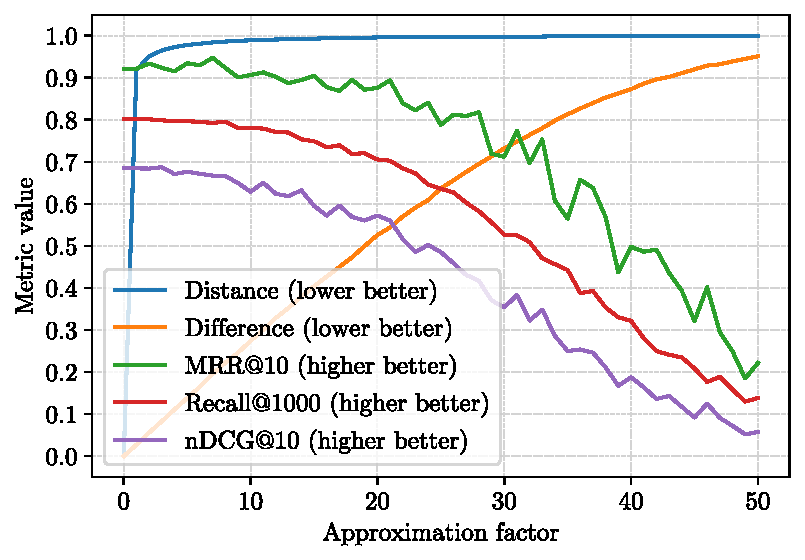
\includegraphics[width=1.0\textwidth]{knn-search-0-50} % chktex 8
	\caption{Search accuracy for $\beta \in \{ 0.0, \ldots, 50.0 \}$}\label{figure:knn-search-coarse}
\end{figure}


				We have run two sets of experiments to see how these metrics change with varying security parameter $\beta$.
				For first set of $\beta$ values, we ranged the parameter from 0 to 50 with increment of $1.0$, see \cref{figure:knn-search-coarse}.
				Higher values of $\beta$ predictably degraded the search accuracy, but we wanted to see how quickly and since which values of $\beta$ the accuracy starts to fall noticeably.

				First, we notice that the result difference grows close to linearly with $\beta$, which means that each new security level knocks out a few correct response from the set proportionally.
				Second, we see that the result distance jumps immediately to almost \SI{100}{\percent}, which means that even tiny approximation term significantly perturbs the order of the responses, but not given low difference, not the content of the result.
				Finally, we observe that at about $\beta = 9$, the \acrshort{trec} metrics start to fall sharply and throughout the entire range of $\beta$ they fall in accord.

				For the maximum vector length of 11, the $\beta$ value that hides half of the input bits is $\beta = \sqrt{11} \approx 3.3$.
				To see the metrics behavior at around this point, we ran the experiments again, now ranging $\beta$ in finer manner, from $0.0$ to $5.0$ with the increment of $0.1$, see \cref{figure:knn-search-fine}.
				We confirm that for $\beta = \sqrt{\max N}$, the values of the ranking quality metrics are sufficiently close to the plaintext values.
				\emph{We therefore conclude that protection \acrshort{dcpe} offer comes cheap in terms of search accuracy.}

				\begin{figure}[h]
	\centering
	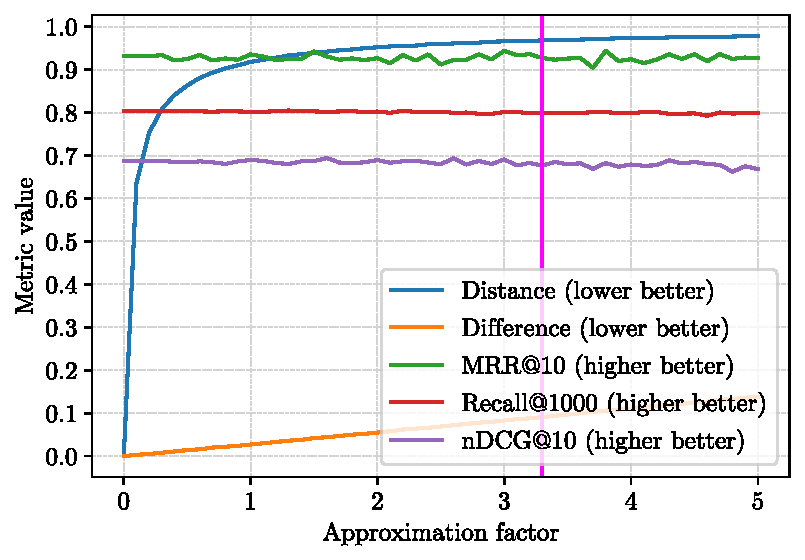
\includegraphics[width=1.0\textwidth]{knn-search-0-5}  % chktex 8
	\caption[Search accuracy for $\beta \in \{ 0.0, \ldots, 5.0 \}$]{
		Search accuracy for $\beta \in \{ 0.0, \ldots, 5.0 \}$.
		{\color{magenta}Highlighted} is $\beta = \sqrt{\max N}$ for $\max N \approx 11$ being the longest vector in the dataset.
	}\label{figure:knn-search-fine}
\end{figure}


	\section{Security against attacks}\label{section:knn-snapshot:attacks}

		The second part of a practical and secure outsourced similarity search application is the protection against attacks.
		In this set of experiments we adapt a recent \acrshort{ml}-based attack by \textcite{embedding-attacks}.
		\textcite{embedding-attacks} offer three attacks against the text embeddings:
		\begin{enumerate*}[label={(\roman*)}]
			\item \emph{the inversion attack}, which recovers a set of words from a document embedding,
			\item \emph{the attribute inference attack} that recovers some property of the document by its embedding, such as the gender or age of its author, and
			\item \emph{the membership inference attack}, which reveals whether a given document was or was not in the training set for the embedding model.
		\end{enumerate*}
		The inversion attack can be run in two modes, the white-box and the black-box.
		The white-box attack assumes the access to an embedding model and therefore can directly use its architecture and parameters to invert the inputs.
		The black-box attack relies only on being able to use the model to produce an embedding from a document, similar to how a generic embedding \acrshort{api} would work.
		We use this latter black-box inversion attack in our experiments since it most closely matches the adversary capabilities in our outsourced database setting.

		\subsection{Black-box model inversion attack \texorpdfstring{\cite{embedding-attacks}}{}}

			The black-box inversion attack assumes no knowledge of the embedding model, it can only use it to produce the embeddings.
			In this section we follow the original notation from \cite{embedding-attacks}.

			The attack works by training another model $\Upsilon$ to recognize the correlation between the set of words $\mathcal{W}(x)$ of a document $x$ and its embedding $\Phi(x)$.
			The attacker uses some auxillary dataset $\database_\text{aux}$ (same domain works predictably better than cross domain), and produces a collection of $ ( \Phi(x), \mathcal{W}(x) ) $ for all $x \in \database_\text{aux}$.
			The adversary then trains the attack model $\Upsilon$ to maximize $ \log \Pr_\Upsilon ( \mathcal{W}(x) | \Phi(x) ) $ over dataset $ ( \Phi(x), \mathcal{W}(x) ) $.
			Finally, the adversary simply queries the model with the embedding $ \Upsilon( \Phi( x ) ) $ and recovers the original words $\mathcal{W}(x)$.

			\textcite{embedding-attacks} offer two models for the inversion attack.
			The \acrfull{mlc} model assigns a binary label of whether a word is in the set for each word in the dictionary.
			The objective function is
			\[
				\mathcal{L}_{\text{\acrshort{mlc}}} = -\sum_{ w \in \mathcal{V} } \left[ y_w \log( \hat{y}_w ) + (1 - y_w) \log(1 - \hat{y}_w) \right]
			\]
			where
			\begin{itemize}
				\item $\mathcal{V}$ is a set of possible words, a dictionary,
				\item $\hat{y}_w = \Pr_\Upsilon( y_w | \Phi( x ) )$ is the predicted probability of word $w$ given $\Upsilon$ conditioned on $\Phi( x )$, and
				\item $y_w = 1$ if word $w$ is in $x$ and 0 otherwise.
			\end{itemize}

			A disadvantage of \acrshort{mlc} model is that it predicts all words independently.
			\textcite{embedding-attacks} therefore offer a more sophisticated approach based on \cite{msp}.
			A \acrfull{msp} recurrent neural network predicts the next word in the set conditioned on the embedding $\Phi( x )$ and the up to date predicted set of words.
			The objective function is
			\[
				\mathcal{L}_{\text{\acrshort{msp}}} = \sum_{ i = 1 }^\ell \frac{1}{| \mathcal{W}_i |} \sum_{w \in \mathcal{W}_i } - \log \Pr_\Upsilon( w | \mathcal{W}_{ < i }, \Phi( x ) )
			\]
			where $\mathcal{W}_{ < i }$ is the set of already predicted words up to a timestamp $i$ and $\mathcal{W}_i$ is the set of words left to predict.
			According to experiments in \cite{embedding-attacks}, \acrshort{msp} outperforms \acrshort{mlc}.

		\subsection{Experimental evaluation}\label{section:knn-snapshot:attacks:experiments}

			We have contacted the authors of \cite{embedding-attacks} and obtained a prototype code they used to run the attack.\footnote{
				\url{https://github.com/google/embedding-tests}
			}
			The model $\Upsilon$ is implemented as a one-layer \acrshort{lstm} with \num{300} hidden units.
			the model is trained for 30 epochs with Adam optimizer \cite{adam-optimizer}, learning rate of $10^{-3}$ and batch size of 256.
			The actual implementation uses TensorFlow \cite{tensorflow} (version 1) and is naturally optimized for \acrshort{gpu} training.

			We run two sets of experiments corresponding to two adversarial settings.
			First, similar to \cite{embedding-attacks}, we assume that the adversary has a black-box access to the embedding model $\Phi$ and can use it to train $\Upsilon$, and we call this experiment an \emph{public model}.
			This setting corresponds to a scenario when the system uses some open embedding model with little to no alterations (i.e., Google AI Platform Training\footnote{
				\url{https://cloud.google.com/ai-platform/training/docs/algorithms/bert}
			}).
			Second, we assume a more realistic scenario where the embedding model $\Phi$ is not available, and the adversary can only use the system as a whole.
			That is, for a given document $x$, the adversary can only produce the encrypted embedding $\algo{Enc}{\Phi(x)}$.
			We call this experiment a \emph{private model}.
			In both experiments the actual outsourced database is encrypted and the difference is in the dataset $\database_\text{aux}$ on which the adversary can train the attack model $\Upsilon$.
			In the public model experiment the adversary trains on plaintext embeddings while in the private model environment she trains on the already encrypted embeddings.

			For both experiments we have used two datasets.
			The first dataset is a BookCorpus \cite{bookcorpus} that \textcite{embedding-attacks} used.
			With this dataset we have been able to verify that our adapted attack implementation produces similar results to original \cite{embedding-attacks}.
			The second dataset is the \acrshort{trec}, same as in \cref{section:knn-snapshot:search}.
			With this dataset we can link together the search accuracy and attack efficiency for the same levels of security.

			\subsubsection{Attack efficiency metrics}

				In line with \cite{embedding-attacks}, we define the attack efficiency metrics similar to a generic \acrshort{ml} measurers of accuracy --- precision, recall and \FOne{} score.
				Precision in our setting is defined as the number of words that the model predicted and that are part of an embedded sentence (i.e., true positives) over the total number of predicted words (all positives).
				Recall is defined as the number of correctly predicted words (true positives) over the number of all words in the sentence (true positives plus false negatives).
				\FOne{} score is then the harmonic mean of these two:
				\[
					\FOne = 2 \cdot \frac{ \mathsf{precision} \cdot \mathsf{recall} }{ \mathsf{precision} + \mathsf{recall} }
				\]

				We go a step further in this direction and given the context of the model --- recovering a set of words from a sentence embedding --- also track the fraction of common words (a.k.a., stop-words) in the predicted set.
				\acrshort{bert} explicitly encourages including the stop-words in the input because their relative position matters for the context and thus embedding.
				However, the attack only produces an unordered set of words and not their relative position.
				Therefore, the \emph{model prediction quality}, the \FOne{} score, may seem high, but it may not imply high \emph{attack efficiency}, because a huge fraction of predicted words are common and thus contribute little to added adversary knowledge.
				We define the list of stop words as pronouns, verb forms of ``be'', ``have'' and ``do'', some modal verbs, compound forms (e.g., ``you'll''), negations, articles, certain prepositions, conjunctions, adverbs and some more high-frequency words.\footnote{
					The list is adapted from the Snowball processing language: \url{http://snowball.tartarus.org/algorithms/english/stop.txt}.
				}
				We also include punctuation and digits to the list, as \acrshort{bert} tokenizes these along with the rest of the words.

			\subsubsection{Baselines}\label{section:knn-snapshot:attacks:experiments:baselines}

				\begin{figure}[h]
	\centering
	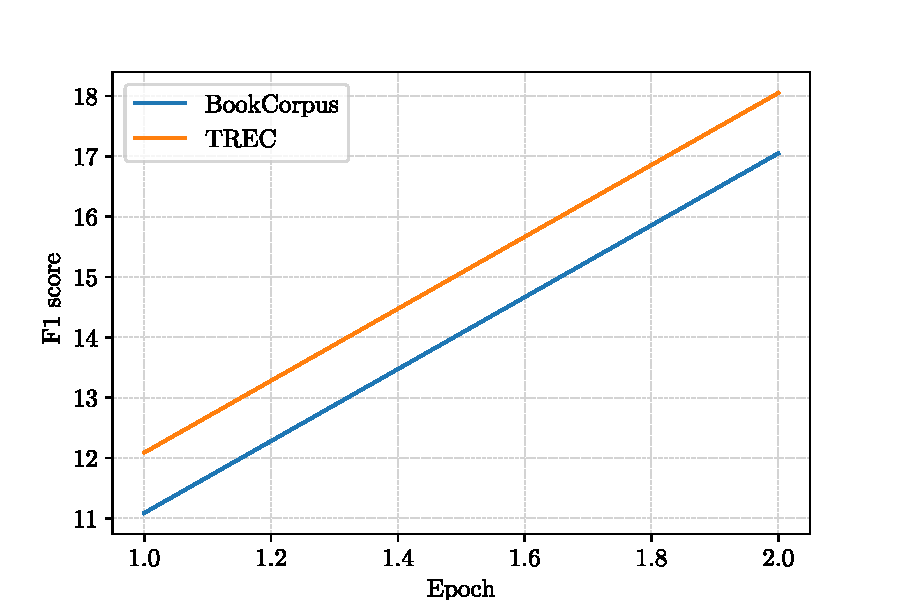
\includegraphics[width=1.0\textwidth]{knn-epochs} % chktex 8
	\caption[Inversion attack F1 score for different epochs]{
		Inversion attack F1 score for different epochs and for both datasets.
	}\label{figure:knn-epochs}
\end{figure}


				We have established two baselines between which the attack performance over encrypted inputs will lie.
				The first baseline is the attack on the plaintext inputs (referred to as \emph{plaintext attack}), a replica of the original attack from \cite{embedding-attacks}.
				The second baseline is the attack on the random embeddings (referred to as \emph{random attack}), which, counterintuitively, does not produce close to zero \FOne{} score.

				In both cases, we have trained the attack model for 30 epochs, see \FOne{} score on \cref{figure:knn-epochs}.
				We note a number of observations:
				\begin{enumerate*}[label={(\roman*)}]
					\item we have replicated the efficiency result of the black-box model inversion attack from \cite[Table 2, \FOne{} score, same domain, $\mathcal{L}_{\text{\acrshort{msp}}}$, \acrshort{bert}]{embedding-attacks},
					\item for the plaintext attack, the \FOne{} score grows stops growing after about $10_\text{th}$ epoch,
					\item the random attack produces a far-from-negligible \FOne{} score,
					\item \acrshort{trec} dataset is much less susceptible to the attack than the originally used BookCorpus.
				\end{enumerate*}

				On this latter observation, we speculate that the reason is in the size of the input document, and to the lesser extent different embedding mechanism.
				BookCorpus input document, as used in \cite{embedding-attacks}, is merely a sentence, while \acrshort{trec} document is a larger paragraph.
				We have tuned the maximum token sequence length (shorter sequences are padded, larger one truncated), but it yielded no improvement.
				From purely combinatorial perspective, we conclude that the larger input looses more information while being embedded in the same-sized vector.

				The case of random attack is puzzling, as one would expect that there is no information to recover from an a-priori information-less (random) inputs.
				We have dived deeper than \FOne{} score and inspected the actual words that the attack recovered and observed that almost all of them are stop-words and punctuation.
				That is, the attack merely established that the input document contained a period, coma, ``the'' and ``a'', and it happened to be right some of time.
				While such inversion technically results in a \SI{30}{\percent} \FOne{} score, it does not necessarily translate into an information leakage or a privacy violation.
				We therefore include an evaluation of recovered words as part of our larger analysis.

				We have run all experiments for both BookCorpus and \acrshort{trec} datasets, and we have noticed that although the absolute values of attack efficiency are higher for BookCorpus, all relations and correlations are the same for both datasets.
				We therefore report on the more relevant \acrshort{trec} dataset in the rest of the chapter.

			\subsubsection{Public model}

				For the public model setting we have used the trained model $\Upsilon$ from the baseline experiments and ran it against the encrypted embeddings.
				That is, for all documents $x$ in $\database_\text{aux}$, we recovered a set of words from the encrypted embeddings $\Upsilon( \algo{Enc}{ \Phi(x) } )$ and compared it to the set of words in the original document $\mathcal{W}(x)$.
				We have repeated the process for different values of $\beta \in \{ 1.0, \ldots, 50.0 \}$, see \cref{figure:knn-public}.

				\begin{figure}[h]
	\centering
	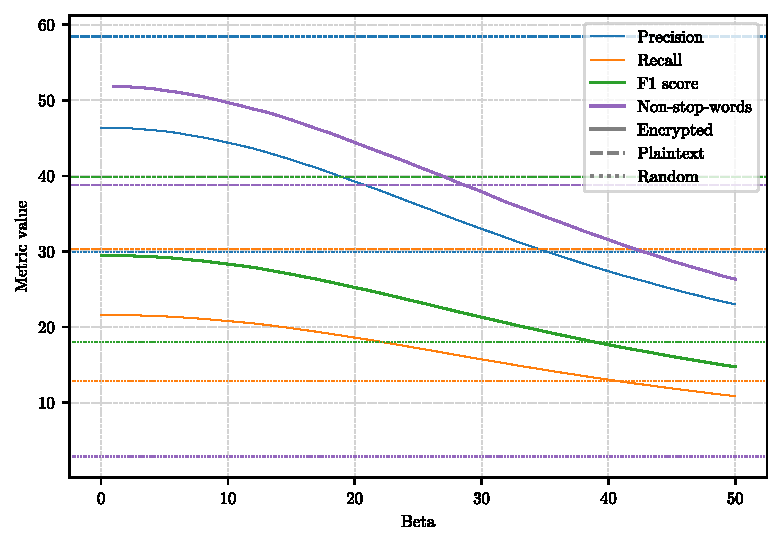
\includegraphics[width=1.0\textwidth]{knn-public} % chktex 8
	\caption[Inversion attack accuracy metrics for different $\beta$ for \acrshort{trec} dataset]{
		Inversion attack {\color{MatplotlibOne}precision}, {\color{MatplotlibTwo}recall}, {\color{MatplotlibThree}\FOne{} score} and {\color{MatplotlibFive}percentage of stop-words among recovered words} for plaintext attack (dashed), random attack (dotted) and different values of $\beta$ (solid) for the \acrshort{trec} dataset.
		Horizontal bars depict the baselines.
	}\label{figure:knn-public}
\end{figure}


				We observe that even for $\beta = 0$, the attack efficiency drops sharply compared to the plaintext baseline.
				We also see that the metric values drop further as $\beta$ increase, starting slowly for small $\beta$, then accelerating for $\beta$ 10 to 30 and than slowing down again as the values get close to the random baseline.
				Finally, we note that the fraction of stop-words grows fast as the security increases.

			\subsubsection{Private model}

				For the private model experiments we have trained the model $\Upsilon$ on the already encrypted embeddings for 30 epochs.
				That is, the model $\Upsilon$ is trained on $ ( \algo{Enc}{ \Phi(x) }, \mathcal{W}(x) ) $ pairs from the training dataset and then we run predictions for the auxillary encrypted embedding, similar to public model.
				The training and validation datasets are encrypted with the same set of public and private parameters (i.e., same key \key{}, $s$ and $\beta$).

				\begin{table}[!ht]
	\renewcommand{\arraystretch}{1.2}
	\sisetup{detect-all = true}
	\begin{tabular*}{\linewidth}{ !{\extracolsep\fill} l c c >{\bfseries}c c } % chktex 26
		\toprule
			Dataset (encrypted with $\beta$)	& Precision				& Recall				& \FOne{} score 		& Non-stop-words		\\
		\midrule
			$\beta = 0$							& \SI{41.59}{\percent}	& \SI{23.36}{\percent}	& \SI{29.91}{\percent}	& \SI{3.67}{\percent}	\\
			$\beta = \ceil{\sqrt{\max N}} = 4$	& \SI{41.91}{\percent}	& \SI{23.75}{\percent}	& \SI{30.32}{\percent}	& \SI{4.96}{\percent}	\\
			$\beta \approx \max N = 11$			& \SI{40.82}{\percent} 	& \SI{24.20}{\percent} 	& \SI{30.39}{\percent}	& \SI{5.18}{\percent}	\\
			$\beta \approx 2 \cdot \max N = 22$	& \SI{40.44}{\percent} 	& \SI{23.75}{\percent} 	& \SI{29.92}{\percent}	& \SI{5.76}{\percent}	\\
		\midrule
			Random embeddings					& \SI{35.91}{\percent}	& \SI{26.49}{\percent}	& \SI{30.49}{\percent}	& \SI{0}{\percent}		\\
		\bottomrule
	\end{tabular*}
	\sisetup{detect-none = true}
	\caption[Inversion attack performance for the private model experiments]{
		Black-box inversion attack performance for the private model experiments.
		The attack model $\Upsilon$ is both trained and validated on the specified datasets.
	}%
	\label{table:knn-private}
\end{table}


				We have chosen the $\beta$ values of $0.0$ and $4.0$ as well as random embeddings to produce the datasets, see \cref{table:knn-private}.
				We immediately notice that the attack model accuracy metrics are similar among all three datasets, with $\beta = 4.0$ and random being almost equal.
				This result implies that for the case of private model --- when the adversary has only black-box access to the system as a whole --- the protection by the \acrshort{dcpe} is absolute.

	\section{Search accuracy against security tradeoff}

		Equipped with the empirical data from experiments on search accuracy and attack efficiency, we can correlate these values with the security parameter, the approximation term $\beta$.

		\begin{figure}[h]
	\centering
	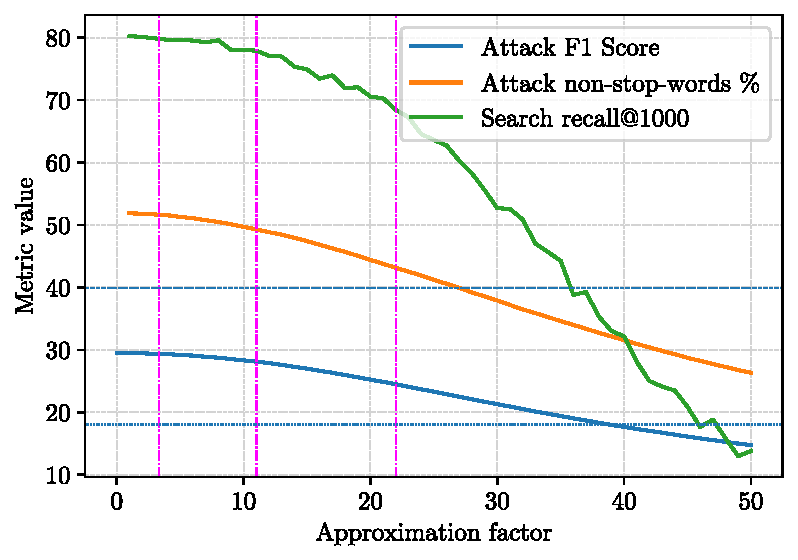
\includegraphics[width=1.0\textwidth]{knn-tradeoff} % chktex 8
	\caption[The correlation of search accuracy and the attack efficiency with $\beta$]{
		The correlation of search accuracy (the {\color{MatplotlibThree}recall@1000}) and the attack efficiency (the {\color{MatplotlibOne}\FOne{} score} and the {\color{MatplotlibTwo}percent of non-stop-words}) with the approximation term $\beta$.
		The {\color{magenta}vertical bars} show special values of $\beta$: $\sqrt{\max N}$, $\max N$ and $2 \cdot \max N$ for $\max N \approx 11$ being the longest vector in the dataset.
	}\label{figure:knn-tradeoff}
\end{figure}


		% TODO: axis 10pt, legend 8 pt.
		% TODO: fix manual constants in plots.


	\section{Conclusions and future work}

		Try other attacks.






	\cleardoublepage%
	\section{Remarks and conclusion}\label{sec:conclusion}

	Having done theoretical and practical evaluations of the protocols, we have found that primitive usage is a much better performance measure than the plain time measurements.
	When it comes to practical use, the observed time of a query execution is a mix of a number of factors and {\IO} requests can slow the system down dramatically.

	ORE-based {\BPlus} tree protocol is provably {\IO} optimal and can potentially be extended by using another data structure with ORE\@.
	Its security/performance trade off is tunable by choosing and parametrizing the underlying ORE scheme.
	Each scheme we considered has its own unique advantages and drawbacks.
	BCLO \cite{bclo-ope} is the least secure scheme in the benchmark, but is stateless and produces numerical ciphertexts, so it may be used in the databases without any modifications.
	Frequency-hiding OPE \cite{fh-ope} also has this property, hides the frequency of the ciphertexts, but is stateful and requires uniform input.
	Lewi-Wu \cite{lewi-wu-ore} is easily customizable in terms of tuning performance to security ratio, and it offers the security benefits of left / right framework --- particuarly useful for {\BPlus} tree.
	CLWW \cite{clww-ore} provides weaker security guarantees but is the fastest scheme in the benchmark.

	Kerschbaum protocol \cite{florian-protocol} offers semantically secure ciphertexts, hiding the location of the smallest and largest of them, and has a simple implementation.
	The protocol is well-suited for bulk insertions and scales well.

	\balance%

	POPE \cite{pope} offers a ``deferred'' {\BPlus} tree implementation.
	By deferring the sorting of its ciphertexts, POPE remains more secure for the small number of queries.
	POPE has the fastest insertion routine and does not reveal the order of most of its ciphertexts.
	It will be more performant for the systems where there are a lot more insertions than queries.
	We would also recommend to ``warm up'' the structure to avoid a substantial delay upon the first query.

	Logarithmic\hyp{}BRC is a perfect choice for huge datasets where query result size is limited.
	It is the only protocol with substantial space overhead, but it offers scalability and perfect (in a snapshot setting) security,
	and a carefully chosen and configured SSE scheme ensures that {\IO} grows slowly as a function of result size.

	ORAM has shown the most interesting result.
	Its performance is not only adequate, but also in-line with the other even less secure protocols.
	With this empirical result, we expect more interest in ORAM research, possibly discovering tighter bounds, faster constructions and efficient ways to use the schemes.
	The performance of ORAM gives an upper bound on the acceptable performance level of less secure (access pattern revealing) protocols, as practitioners will choose ORAM over both less secure and less performant solutions.

	We found our framework to be a powerful tool for analyzing the protocols, and we hope developers of new protocols will contribute implementations and evaluate them.

	An important future work is to understand better the meaning of the different leakage profiles and their implications.
	Furthermore, another direction is to try to improve the performance of the most secure schemes (e.g. \cite{parameter-hiding-ore}). % chktex 2

	\cleardoublepage%

	% \begin{appendices}



	% \end{appendices}

	\newpage
	\singlespace%

	\phantomsection%
	\addcontentsline{toc}{chapter}{Bibliography}

	\printbibliography%

	\cleardoublepage%

	\phantomsection%
\addcontentsline{toc}{chapter}{Curriculum \texorpdfstring{Vit\ae}{Vitae}}

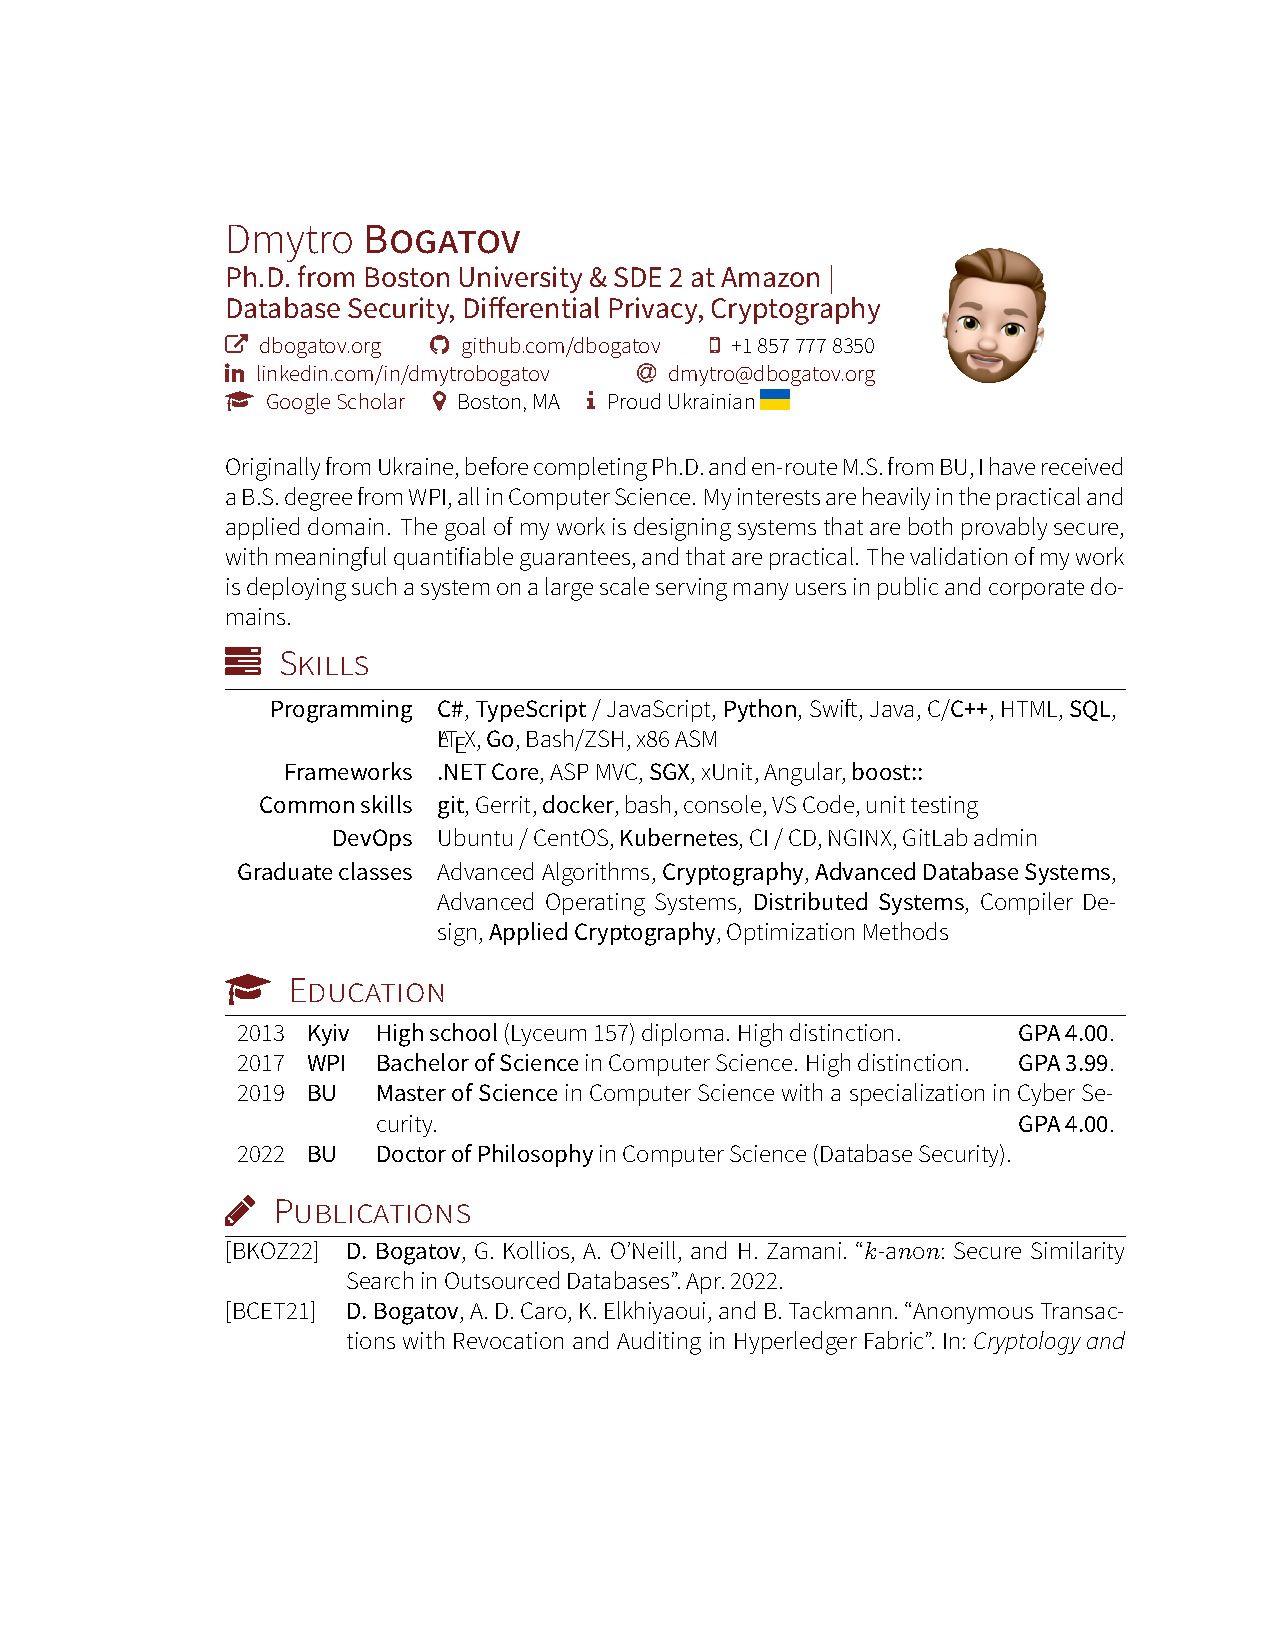
\includepdf[
	pages=-,
	pagecommand={},
	width=0.98\paperwidth,
	offset=-18 18 % horiszontal vertical
]{graphics/cv.pdf}


\end{document}
